\documentclass[11pt,twoside]{report}
\usepackage[dvips]{graphics}
%\includeonly{ballisti}   %intro, analysis, freefall, reaction, project, atwood,
%twobody,kinetic, rotation,harmonic,pendulum,appa, appb, appc, appd}
\setlength{\unitlength}{0.025in}
%\input setbmp
\newcommand{\delete}{\(<\)\begin{picture}(8,4.2)
                     \put (-0.6,-0.1){\line(1,0){4.5}}
                     \put (3.9,-0.1){\line(0,1){3}}
                     \put (-0.6,2.9){\line(1,0){4.5}}
                     \put (1.4,1.4){\makebox(0,0){x}}
                     \end{picture}}
\newcommand{\sine}{\begin{picture}(8,5)(0,-1)
                  \put(2,0.5){\oval(3,4)[b]}
                  \put(5,0.5){\oval(3,4)[t]}
                  \end{picture}}
\newcommand{\cnum}[1]{\begin{picture}(8,5)(0,-1)
                  \put(4,0.5){\makebox(0,0){{\small {#1}}}}
                  \put(4,0.5){\circle{6}}
                  \end{picture}}
\newcommand{\newexp}{\cleardoublepage
                     \addtocounter{chapter}{1}
                     \setcounter{equation}{0}
                     \setcounter{figure}{0}
                     \chapter*{EXPERIMENT \# \thechapter:\ \newname}
                     \markboth{\exphead}{\exphead}
                     \addcontentsline{toc}{section}{\newname}}
\newcommand{\newapp}{\cleardoublepage
                     \addtocounter{chapter}{1}
                     \setcounter{equation}{0}
                     \setcounter{figure}{0}
			   \setcounter{table}{0}	%added CAG, July 98
		     \chapter*{\newname}
                     \markboth{\apphead}{\apphead}
                     \addcontentsline{toc}{section}{\newname}}
\newcommand{\exphead}{\hspace*{\fill} \underline{EXPERIMENT \#\thechapter:\
                      \newname} \hspace*{\fill}}
\newcommand{\apphead}{\hspace*{\fill} \underline{\newname} \hspace*{\fill}}
\newcommand{\nc}{\newcommand} \nc{\rnc}{\renewcommand}
\nc{\bc}{\begin{center}} \nc{\ec}{\end{center}}
\nc{\be}{\begin{enumerate}} \nc{\ee}{\end{enumerate}}
\nc{\bi}{\begin{itemize}} \nc{\ei}{\end{itemize}}
\nc{\bt}{\begin{tabular}} \nc{\et}{\end{tabular}}
\nc{\beq}{\begin{equation}} \nc{\eeq}{\end{equation}}
\nc{\beqa}{\begin{eqnarray}} \nc{\eeqa}{\end{eqnarray}}
\nc{\bfig}{\begin{figure}} \nc{\efig}{\end{figure}}
\nc{\bpic}{\begin{picture}} \nc{\epic}{\end{picture}}



\pagestyle{headings}
\textwidth=6in
\textheight=9.25in
\topmargin=-0.5in 				% + 1 3/8 in  = 7/8
\oddsidemargin=.25in 				% + 1 in      = 1.25
\evensidemargin=.25in 				% + 1 in      = 1.25
\parindent=0in					% no indent
\parskip=2ex					% skip lines
\flushbottom
\title{{\Huge {\bf Laboratory Manual for \\ Foundations of Physics I}}}
\author{{\LARGE Physics 191}}
\date{{\Large Fall 2003}}
\begin{document}
\maketitle
\tableofcontents
\setcounter{chapter}{-1}
\newcommand{\newname}{Introduction}
% INTRODUCTION
\newapp
\section*{Purpose}

\begin{quote}
When you measure what you are speaking about, and express it in numbers,
you know something about it, but when you cannot express it in numbers,
your knowledge is of a meager and unsatisfactory kind: It may be the beginning 
of knowledge, but you have scarcely in your thoughts advanced to
the stage of science.  {\em Lord Kelvin}
\end{quote}


Physics and engineering rely on quantitative experiments.
Experiments are artificial simplifications of nature:
line drawings rather than color photographs.  The hope is that by striping away
the details, the essence of nature is revealed.  
Although the aim of experiment is appropriate 
simplification, the design of experiments is anything but simple.
Typically it involves days (weeks, months, \ldots) of ``fiddling"
before the experiment finally ``works".  I wish this sort of creative
problem-oriented process
could be taught in a scheduled lab period to incoming students,
but limited time and the many prerequisites make this impossible.
(You have to work on grammar before you can write the great American
novel.)  Look for more creative labs starting next year!

%Rejecting magic, we assume that nature is consistent, and further that
%we are equipped to discover the (mathematical) rules
%that nature follows.  (The critics of science would note the hubris
%is this statement.)  

Thus this lab manual describes experiences (``labs")
that are caricatures of experimental physics.
Our labs will typically 
emphasize thorough preparation, an underlying mathematical
model of nature, good experimental technique, analysis
of data (including the significance of error)
\ldots the basic prerequisites for doing science.
But your creativity will be circumscribed.  You will find here ``instructions"
that are not a part of real experiments (where the methods and/or  outcomes
are not known in advance).  

The goals of these labs are therefore limited.  You will:
\begin{enumerate}
\item Perform certain experiments that illustrate the foundations of 
Newton's mechanics. 
\item Perform basic measurements and recognize the associated limitations
(which, when expressed as a number, are called uncertainties or errors).
\item Practice the methods which allow you to determine how uncertainties 
in measured quantities propagate to produce uncertainties 
in calculated quantities.
\item Practice the process of verifying a mathematical model,
including data collection, data display, and data analysis (particularly
graphical data analysis with curve fitting).
\item Practice the process of keeping an adequate lab notebook.
\item Experience the process of ``fiddling" with an experiment until it finally
``works".
\item Develop an appreciation for the highs and lows of lab work.
And I hope: learn to learn from the lows.
\end{enumerate}

\section*{Semester Lab Schedule}
To be announced in class.  Note that this Manual does not list
labs in the scheduled order.

You should be enrolled in a lab section for PHYS 191.  Your labs will
be completed on the cycle day/time for which you have enrolled.  These are
the only times that the equipment and assistance will be available to
you.  It is your responsibility to show up and complete each
lab.  (Problems meeting the schedule should be 
addressed---well in advance---to the lab manager.)

\section*{Materials}
You should bring the following to each lab:
\begin{itemize}
\item Lab notebook.  You will need three notebooks: While one is being
graded, the others will be available to use in the following labs.  The lab
notebook should have quad-ruled paper (so that it can be used for
graphs) and a sewn binding (for example, Ampad \#26--251, available in
the campus bookstores).
%
  \item Lab Manual (this one)
%
  \item The knowledge you gained from carefully reading the lab manual
  before you attended.
  \item A calculator, preferably scientific.
  \item A straightedge (for example, a 6" ruler).
\item A pen (we strongly prefer your lab book be written in
ink, since one should {\bf never}, under any circumstances, erase).
However, pencils are ok for drawings and graphs.
%  \item A 3.5" floppy disk to save your data.  (However, see the
%  last section of the Introduction for other options for saving
%  your data.)
\end{itemize}

%\section*{Open Lab System}
\section*{Before Lab:}

     Since you have a limited time to use equipment (other
students will need it), it will be to your advantage
if you come to the laboratory well prepared.  Please read the
description of the experiment carefully, and do any preliminary work
{\em in your lab notebook} before you come to lab.   (The section below
headed ``Lab Notebook'' gives a more complete description of what to
include in your lab notebook.)

There may be one or more quizzes
sometime during the semester to test how well you prepared for the lab.
These quizzes, as well as the pre-lab assignments, will be collected during
the FIRST TEN MINUTES of lab, so it is wise to show up on time or early.

\section*{During Lab:}

Note the condition of
your lab station when you start so that you can return it to that state when you leave.
Check the apparatus assigned to you.  Be sure you know the function of
each piece of equipment and that all the required pieces are present.
If you have questions, ask your instructor.  Usually you will want
to make a sketch of the setup in your notebook.
Prepare your
experimental setup and decide on a procedure to follow in
collecting data.  
Keep a running outline in your notebook of the procedure actually used.
If the procedure used is identical to that in this Manual,
you need only note ``see Manual".  Nevertheless, an outline of your
procedure can be useful even if you aim to exactly follow the Manual.
Prepare
tables for recording data (leave room for calculated quantities).
{\em Write your data in your notebook as you collect it!}  

Check your data table and graph, and make sample calculations if
pertinent to see if everything looks satisfactory before going on
to something else.  Most physical quantities will appear to vary
continuously and thus yield a smooth curve.  If your data looks
questionable (e.g., a jagged, discontinuous ``curve") you should take
some more data near the points in question.  Check with the instructor 
if you have any doubts.

Complete the analysis of data in your notebook and
 indicate your final results clearly.  If you make repeated calculations
 of any quantity, you need only show one sample calculation.  
Often a spreadsheet will be used to make repeated calculations.
In this case it is particularly important to report how each column was
calculated.  
Tape computer-generated data tables, plots and least-squares fit
reports into your notebook, so that they can be examined
easily.  Answer all questions that were asked in the Lab Manual.

{\bf CAUTION:}  {\em for your protection and for the good of the
equipment, please check with the instructor before turning on
any electrical devices.}

 \section*{Lab Notebook}

Your lab notebook should represent a {\em detailed} record of what
you have done in the laboratory.   It should be complete enough
so that you could look back on this notebook after a year or two and
reconstruct your work.    Sample notebook
pages from a previous student are included at the end of this
section.

     Your notebook should include your preparation for lab,
sketches and diagrams to explain the experiment, data collected,
initial graphs (done as data is collected), comments on
difficulties, sample calculations, data analysis, final graphs,
results, and answers to questions asked in the lab manual.  {\bf
NEVER} delete, erase, or tear out sections of your notebook that
you want to change.  Instead, indicate in the notebook what you
want to change and why (such information can be valuable later on).
Then lightly draw a line through the unwanted section and proceed with
the new work.

{\bf DO NOT} collect data or other information on other sheets
of paper and then transfer to your notebook.  Your notebook
is to be a running record of what you have done, not a formal
(all errors eliminated) report.  There will be no formal lab
reports in this course.  When you have finished a particular lab, you turn in
your notebook at the end of the period.

Ordinarily, your notebook should include the following items for each
experiment.

\begin{description}
\item {\bf NAMES}.  The title of the experiment, your name, your
lab partner's name, and your lab station number.

\item {\bf DATES}.  The date the experiment was performed.

\item {\bf PURPOSE}.  A brief statement of the objective or purpose of the
experiment.

\item {\bf THEORY}.  At least a listing of the relevant equations, and what the symbols
represent.  Often it is useful to number these equations so you can
unambiguously refer to them.

{\bf Note:}  These first four items can usually be completed before
you come to lab.  

\item {\bf PROCEDURE}.  This section should be an outline of
what you did in lab.  
As an absolute minimum your procedure must clearly describe
the data.  For example, a column of numbers labeled ``voltage"
is not sufficient.  You must identify how the voltage was measured,
the scale settings on the voltmeter, etc.  Your diagram of the
apparatus (see below) is usually a critical part of this
description, as it is usually easier to draw how the data
were measured than describe it in words.  Sometimes
your procedure will be identical to that
described in the lab manual, and it's OK to say simply so.
However there are usually
details you can fill in about the procedure.  Your procedure
may have been different from that described in the lab manual.
Or points that seem important to you may not have been included.
And so on.  This section is also a good place to describe any
difficulties you encountered in getting the experiment set up and
working.

\item {\bf DIAGRAMS}.  A sketch of the
apparatus is almost always required.  A simple block diagram can often describe the
experiment better than a great deal of written explanation.

\item {\bf DATA}.  You should record {\em all} the numbers
you encounter,
including {\em units} and {\em uncertainties}, and any other relevant
observations  as the experiment progresses.  The lab
report should include the {\em actual} data taken in the lab, not
recopied versions.  If you find it difficult to be neat and organized while
the experiment is in progress, you might try using the left-hand pages of
your notebook for doodles, raw data, rough calculations, etc., and later
transfer the important items to the right-hand pages.

This section can also include computer-generated data tables and
Linfit reports if
appropriate---just tape them into your lab book (one per page please).

It's good practice to graph the data as you acquire
it in the lab; this practice allows you to see where more data are
needed
and whether some measurements are suspicious and should be repeated.

\item {\bf CALCULATIONS}.  {\bf Sample calculations} should be included to
show how results are obtained from the data, and how the uncertainties
in the {\em results} are related to the uncertainties in the {\em
data} (see Appendix A).  For example, if you calculate the slope and
intercept of a straight line on a graph, you should show your work
in detail.  Your TA must be able to reproduce your every calculation
just based on your notebook.  The TAs have been instructed to
totally disregard answers that appear without an obvious source.
It is particularly important to remember to show how each column in a
spreadsheet hardcopy was calculated.

\item {\bf RESULTS/CONCLUSIONS}. You should end each experiment with a conclusion that
summarizes your results --- how successful was the experiment, what did
you learn from it, and what were your results (including numerical
results, with experimental errors).

  This section should begin with a
summary of your results, collected in a {\em carefully constructed}
table that summarizes all of your results in one place. Always include
units and experimental error.

You should also compare your results to the theoretical and/or
accepted values.
Does your experimental range of uncertainty overlap the accepted value?
Based on your results, what does the experiment tell you?

\item {\bf DISCUSSION/CRITIQUE}.
As a service to us and future students we would appreciate it if you
would also include a short critique of the lab in your notebook.
  Please
comment on such things as the clarity of the Lab Manual, performance
of equipment, relevance of experiment, and if there is anything you
particularly liked or disliked about the lab.  This is a good place to
blow off a little steam.  Don't worry; you won't be penalized, and we
use constructive criticisms to help improve these experiments.

%\item {\bf QUICK REPORT}.
%As you leave lab, turn in a $3\times5$ ``quick report" card.
%You will be told in lab what information belongs on your card.
%These cards go directly to the Lab Manager who will use them to
%identify problems.

\end{description}

%At the end of most labs in this manual there is a checklist for you to
%use when finishing up the lab.  {\em HINT: it's the same checklist
%your TA will use when grading your work!} It can serve as a guide for
%you so you won't forget some important part of the experiment.  You'll
%usually find an item called ``Cleanup" in each checklist.  Your lab TA
%will check your lab station when you leave.  Equipment, hookups, and
%everything else should appear exactly as it did when you sat down to
%start the lab.

Drop off your Lab Notebook in your Lab Instructor's box. 
Note: {\em The TA's cannot accept late labs. If for some reason you
cannot complete a lab on time, please see the lab manager (Lynn Schultz) in EngelSC 139 or call
363--2835. Late labs will only be accepted under exceptional circumstances.
If an exception is valid, the lab may still be penalized depending on how
responsibly you handled the situation (e.g., did you call BEFORE the lab 
started?).}

\section*{Grading}

Each lab in your notebook will be graded separately as follows: \\
\begin{tabbing}
1234567890123456 \= col2 \kill
9--10 points: \> A \\
8--8.9 points: \> B \\
7--7.9 points: \> C \\
6--6.9 points: \> D \\
0--5.9 points: \> Unsatisfactory \\
\end{tabbing}


%\newpage
%\vspace*{\fill}
\begin{figure}[hbt]
   \centerbmp{6.81in}{9in}{sample.bmp}
 %\caption{CAPTION HERE \label{fig:REFERENCE HERE}}
\end{figure}
\clearpage
%\newpage
%\vspace*{\fill}
\begin{figure}[hbt]
   \centerbmp{6.81in}{9in}{sample2.bmp}
   %\special{bmp:sample2.bmp}
 %\caption{CAPTION HERE \label{fig:REFERENCE HERE}}
\end{figure}
%\newpage
\clearpage


\renewcommand{\newname}{Data Analysis}
% DATA ANALYSIS
\newexp

\section*{Before Lab}
You must make three hand-drawn graphs in your lab notebook
{\bf before} you come to lab: 
\begin{itemize}
\item Data Set 1 --- the graph of distance (on the $y$-axis) vs.\ time (on the
$x$-axis) should look approximately linear.
\item Data Set 2 --- the graph of activity $N$ (on the $y$-axis) vs.\ time (on the
$x$-axis) should look curved.
\item Data Set 2 --- the semi-log graph of $\ln(N)$ (on the $y$-axis) vs.\ time (on the
$x$-axis) should look linear.  Follow the exponential function graphical
analysis outlined on page \pageref{exprel} in Appendix C. 
Provide a table analogous to Table \ref{table:pressure} on page
\pageref{table:pressure} showing the logarithmic transformation of the data and error
in Data Set 2.
\end{itemize}
Each graph should be sized to fill a notebook
page with axes ranges selected to surround the data with a minimum of unused space.
Accurately drawn errors bars (following Figure~\ref{fig:b1}) are required.


One purpose of the first few experiments is to introduce you to
the data reduction and analysis concepts that are described in the
four Appendices to this manual.  You should begin working your way
through these Appendices now---there is a lot in them and it will take
you some time to understand it.

For this experiment you will need to be familiar with at least some
of the material in each of these Appendices:
\begin{itemize}
\item Appendix A (on error analysis) talks about how to estimate uncertainties
in experimentally measured quantities.
\item Appendix B (fairly short) gives you some guidelines on how to make a graph.
Use the graphs in Appendix C as examples.
%
\item Appendix C (on graphical analysis), especially the sections on linear
and exponential functions.  Note especially the logarithmic transformation that we
use to make an exponential function look like a straight line.  You may need
to review the properties of logarithms as you study this section.
%
\item Appendix D on Computer-Assisted Curve Fitting.  We will be making
two least-squares fits on the computer for this experiment, and a good many
more later in the semester.  Appendix D provides an introduction to
the method of least squares and to the computer program we will be
using.
\end{itemize}

Of course, you should also read carefully the writeup for this experiment, given
below.  

%\begin{tabbing}
%reference12345 \= col2 \kill
%References: \> Laboratory Manual, Experimental Error or Uncertainty,
% page~\pageref{scierror} \\
%\> Data Handling, page~\pageref{datahandle} \\
%\> Data Analysis, page~\pageref{datanal} \\
%\> Computer Assisted Curve Fitting, page~\pageref{compassis}
%\end{tabbing}

\section*{Data}
    Much of your work in laboratory this semester will involve
the careful plotting and analysis of experimental data.  In this
exercise you will be given two sets of data and asked to
work with each set.
%\begin{center}
%Data Set 1 \\
%Average Velocity
%\end{center}
\subsubsection*{Data Set 1:  Average Velocity}
     Suppose an airplane on a long flight over a very poorly
mapped route passes over a series of air traffic control radio
beacon checkpoints that have been dropped by parachute.  At each
checkpoint the time is recorded with an accuracy of about 1
second (i.e., better than 0.001 hours).  The distance of each
checkpoint from the plane's starting point is known only to
within about $\pm$150 km.  The following data are recorded:
\newcommand{\Z}{\phantom{0}}
\begin{center}
\begin{tabular}{|cc|}\hline
 & distance from \\
 elapsed time & starting point \\
 (hours $\pm$0.001) & (km $\pm$150) \\ \hline
 0.235 & \Z200 \\
 1.596 & 1200 \\
%1.678 & 1500 \\
 1.921 & 1850 \\
 2.778 & 2100 \\
 3.310 & 2750 \\
 4.314 & 3500 \\
 4.846 & 4200 \\
 6.147 & 4900 \\
 6.678 & 5700 \\
 7.979 & 6650 \\\hline
\end{tabular}
\end{center}
%\begin{center}
%Data Set 2 \\
%Half-life
%\end{center}
\subsubsection*{Data Set 2:  Radioactive Decay}
    The activity of a certain radioactive element is monitored by
a Geiger counter, which clicks and records a ``count" each time it
detects a nucleus undergoing a radioactive decay.  The number $N$ of counts
during a one minute period is recorded along with the start time of
the count.  The estimated uncertainty in a count ($\delta N$) is
$\sqrt{N}$. (Why this is the proper error estimate is explained
in Taylor's {\em An Introduction to Error Analysis}.)  The error in start-time is negligible.
%<<Statistics`DiscreteDistributions`
%Table[Random[PoissonDistribution[2800 E^(- .03 n)]],{n,1,50}]
\begin{center}
\begin{tabular}{|ccc|}
\hline
time & $N$ & $\delta N$ \\
(min) & (counts/min) & (counts/min) \\ \hline
\Z2 & 2523 & 50\\
\Z4 & 1908 & 44\\
\Z6 & 1632 & 40\\
\Z8 & 1263 & 36\\
10  & 1068 & 33\\
12  & \Z861 & 29\\
14  & \Z714 & 27\\
16  & \Z560 & 24\\
18  & \Z452 & 21\\
20  & \Z372 & 19\\ \hline
\end{tabular}
\end{center}
%                FIT                 
% PARAMETER     VALUE      ERROR     
%   A =         0.303E+04   50.      
%   B =        -0.105      0.18E-02  
%\Z2 & 2662 & 52 \\
%\Z6 & 2333 & 48 \\
%10 & 2091 & 46 \\
%14 & 1817 & 43 \\
%18 & 1719 & 41 \\
%22 & 1464 & 38 \\
%26 & 1328 & 36 \\
%30 & 1087 & 33 \\
%34 & 1034 & 32 \\
%38 & \Z886 & 30 \\
%42 & \Z733 & 27 \\
%46 & \Z698 & 26 \\
%50 & \Z649 & 25 \\\hline
%\end{tabular}
%\end{center}
%%                FIT                
%% PARAMETER     VALUE      ERROR     
%%   A =         0.283E+04   41.     
%%   B =        -0.303E-01  0.61E-03 
%% reduced chi-squared of  1.4

%The activity $C$ in
%counts/minute are recorded as a function of time, resulting in
%the following table.  
%The uncertainty in the activity is about
%3\%.
%\begin{center}
%\begin{tabular}{cc|cc}
%time & $C$ & time & $C$ \\
%(min) & (counts/min $\pm$3\%) & (min) & (counts/min $\pm$3\%) \\ \hline
%5.5 & 2410 & 26.5 & 1251 \\
%7.0 & 2284 & 29.5 & 1137 \\
%8.5 & 2188 & 32.5 & 1130 \\
%10.0 & 2038 & 35.5 & 1002 \\
%11.5 & 1959 & 38.5 & 905 \\
%13.0 & 1971 & 41.5 & 786 \\
%14.5 & 1918 & 44.5 & 773 \\
%16.5 & 1756 & 47.5 & 704 \\
%18.5 & 1675 & 50.5 & 687 \\
%20.5 & 1599 & 53.5 & 618 \\
%22.5 & 1464 & 56.5 & 562 \\
%24.5 & 1350 & 59.5 & 478 \\
%\end{tabular}
%\end{center}
%                FIT                      
% PARAMETER     VALUE      ERROR          
%   A =         0.280E+04   37.            
%   B =        -0.290E-01  0.40E-03        

\section*{Analysis}
\subsection*{Graphical Analysis}
Try to complete all four steps given below {\em before} coming to lab.
If you have problems, talk to your instructor, but as a minimum
draw the three required graphs of the above data in your notebook.


\begin{enumerate}
\item In your lab notebook, make a careful graph of each set of
        data, following the guidelines given in
        Appendix B  and using the graphs in
        Appendix C  in the lab
        manual as an example.  Be sure
        you plot the error bars.
\item For the first data set, the graph  of distance vs.\ time
        should be linear.  Draw the best possible line and record
its slope (average velocity, $B$) and $y$-intercept ($A$).

Following the procedure shown in Fig.~\ref{fig:slope} on
page \pageref{fig:slope} draw two additional approximating lines
one with a steeper slope than the best line, and one with a less
steep slope. Find the slope and $y$-intercept of these lines.
Use half the resulting range of
possible slopes to estimate the
uncertainty in average speed ($\delta B$), i.e.,
\[
\delta B = {|B_{\rm max} -B_{\rm min}|\over 2}
\]
Similarly find the
uncertainty in $y$-intercept ($\delta A$).
%       If it is, use the graph to estimate
%        the average speed of the plane.

%        Make careful calculations of the slope and the $y$-intercept
%        of the best line.%, and explain how they are to be interpreted.
%        Use the range of
%        possible slopes allowed by the error bars to estimate the
%        uncertainty in average speed (see Fig.~\ref{fig:slope} in
%Appendix C) and $y$-intercept. %page~\pageref{datanal}).
{\bf Result:} for slope a best value with uncertainty and units; for $y$-intercept
 a best value with uncertainty and units.
\item For the second data set, the graph of activity vs.\ time
        should {\em not} be linear.  Therefore the first step is to
        determine what sort of function describes the data.  Read
        carefully the section in Appendix C on Exponential Function
        (page~\pageref{exprel}) of this lab manual.  Following
        the advice of that section make a semi-log plot of the
        data which should look linear.  Begin by making a table analogous to 
Table \ref{table:pressure} on page
\pageref{table:pressure} showing the logarithmic transformation of the data and error
bars. Again, draw three approximating lines.
Calculate the slope and the $y$-intercept of the best line on the log-transformed plot.
Use half the range of
        possible slopes allowed by the error bars to estimate the
        uncertainty in slope
and $y$-intercept. %page~\pageref{datanal}).
{\bf Result:} for slope ($B$) a value with uncertainty and units; for $y$-intercept
($C$, see Eq.~\ref{eq:transform_line}) a value with uncertainty (no units!).
Calculate the $A$ parameter of the exponential function from $C$ (see Eq.~\ref{eq:transformC}) (report units!).
Use the high-low method (see page \pageref{par:high.low.game}) to find
the uncertainty in $A$.


%        and see if you can find a way of plotting the data that
%        gives you a straight line.  (Hint:  Radioactive materials
%        usually decay exponentially).

%        Note that you can use Linfit, the data analysis and least-squares
%        fitting program we will be using, to make on-screen graphs of
%your
%data quickly and easily.  It may save you a good bit of time if you
%        use the program to investigate the form
%        of the fitting function before plotting the graphs in your
%        lab notebook.
%
\item Is there any way the  exponential parameters can be estimated (however crudely) directly from
non-transformed data?  Yes! The $A$ parameter represents the activity at zero time;
with a bit of extrapolation of the curve one can guess-estimate $A$ from the $y$-intercept.
Exponential functions can be characterized by a ``half-life,'' $\tau$,
in this case the time needed for half of the sample to undergo decay.
To estimate the half-life from your untransformed graph, find
%The half-life can be easily estimated from your untransformed graph.  Find
any two points on the smooth curve (i.e., not data points) such that the activity 
of the second point
is half the activity of the first point.  The time interval between
the two points is the half-life.  Use your graph to make a {\em rough} estimate.
One can then calculate the $B$ parameter from the half-life:

%We can find a more accurate estimate of the half-life by deriving a 
%relationship between it and the $B$ parameter.
If we have two points $(t_1,N_1)$ and $(t_2,N_2)$ such that
$N_2=N_1/2$ and $\tau=t_2-t_1$.  The exponential relation says:
\begin{eqnarray}
N_1&=&A e^{Bt_1}\\
N_2&=&Ae^{Bt_2}
\end{eqnarray}
If we divide the second equation by the first we have:
\begin{equation}
{1\over 2} =  {N_2\over N_1} = {Ae^{Bt_2} \over Ae^{Bt_1}} = e^{B(t_2-t_1)} =
e^{B\tau} 
\end{equation}
If we now take the natural log of both sides we have:
\begin{equation}
\ln\left({1\over 2}\right) = \ln\left(e^{B\tau}\right) = B\tau 
\end{equation}
or
\begin{equation}
B = {\ln\left({1\over 2}\right) \over \tau} 
\end{equation}

On the other hand, you can reverse this equation and use the slope ($B$) of your semilog plot
%Thus if you calculate $B$ using your graph, you can use the result 
to calculate (more accurately) the half-life $\tau$.
Note that this relationship between  $B$ and $\tau$ is contained
in Eq.~\ref{eq:cnew}:
\begin{equation}
B = 
{\ln\left(y_{2}/y_{1}\right) \over x_{2} - x_{1}} =
{Y_{2}-Y_{1} \over x_{2} - x_{1}}
\end{equation}
Use your graphically determined slope $B$ to calculate the half-life $\tau$, and compare it to the value
you found above, from the direct inspection of your untransformed graph. (Don't forget
to include units for $\tau$.)

\end{enumerate}
\subsection*{Computer Analysis}
    In the laboratory we will go over the graphical data analysis
outlined above, and then see how to use the computer to analyze
the same data using the method of least squares (see Appendix D).
{\bf Result:} for each dataset the computer will find values for
parameters $A$  and $B$ (each with an uncertainty).  You will need to
add appropriate units.  Tape the two fit reports and three computer
generated plots into your notebook.


%Feel free to log on to the \WAPP web site\footnote{{\tt http://www.physics.csbsju.edu/stats/WAPP2.html}} 
%and do the on-line analysis at home before you come to lab!

    Before leaving lab, make sure the instructor has checked your
work.

\section*{Lab Writeup}

The Introduction to this lab manual describes what should
usually be included in your notebook, but this experiment is
a bit different.

For this particular experiment, be sure to include the following items:
\begin{enumerate}
\item The four steps outlined above, which constitute your graphical
analysis of the two data sets.
\item The results of your computer analysis for the two data sets.
Tape the fit reports and three graphs into your notebook.  Properly
(sigfigs, error, unit) report the results of each computer fit.

Compare your own graphical analysis calculation of each
$A$ and $B$ parameter to what \WAPP reports.  The 
values should agree within experimental uncertainty.
For the reason cited on page \pageref{par:small.error}, your graphical
estimates of uncertainty may be larger than those found by \WAPP.

\item Using the $B$ parameter found by \WAPP calculate the half-life and its
uncertainty. The calculation of the uncertainty in the
half-life is probably new to you.  You will need to use one
of the formulas in Appendix A
(page~\pageref{errorprop}) of this lab manual (or one in the compendium
of such formulae in Appendix E at the end of this lab manual) to find the
{\em uncertainty} in the half-life in terms of the
uncertainty in the parameter $B$.  
Check with your instructor if you are not
sure how this calculation works.  Compare this calculated
half-life to that found graphically.

\item Conclusions (see below)
\item Critique (see below)
\item $3\times5$ quick report card
\end{enumerate}

\section*{Conclusions}
Your conclusion should include the following:
\begin{itemize}
\item Two tables summarizing the results of your analysis for the
two sets of data (including every calculated $A$ and $B$ value
with proper sigfigs, units and uncertainty).  Place the  the graphically estimated
parameters directly adjacent to the equivalent computer determined parameters so they can
be compared easily.
(Tabulating and comparing results obtained during lab is almost
always part of your conclusion section.)
%
\item Several paragraphs discussing the conclusions you drew from
this analysis.  For example,
\begin{itemize}
\item Did your graphical results and computer least-squares fit results agree, within
      experimental uncertainty?
%
\item How valid and reliable were your least squares fits?  See Appendix D page
\pageref{par:chi_square}
for a discussion of the relationship between reduced
chi-squared and the validity of the fit.
%
\item Any other conclusions you drew from your analysis.
\end{itemize}
\end{itemize}


\subsection*{Critique of Lab}
     Follow the suggestions given in the Introduction to the Laboratory Manual.
You may also want to comment on the relative ease of using the
computer.

\renewcommand{\newname}{Freely Falling Body}
%FREELY FALLING BODY
\newexp

\section*{Before Lab}

Please read this writeup carefully. At many points the writeup asks
questions and reports things
you should address in your notebook (e.g., ``Explain why in your notebook").
A good strategy is to highlight or underline each question mark and ``explain why"
as you read so you can quickly
find them and confirm that you have answered each of them before you turn in your notebook.
Please also continue reading
in the Appendices to this manual.  This experiment particularly stresses
material from Appendices A and D.

\section*{Introduction}
     Two objects with the same size and shape but different mass are
     shown to you.  Then someone asks:
Which will fall faster, the heavy one or the light one?
Aristotle (about 300 B.C.)  gave his philosophical arguments
which concluded that the heavy one fell faster.  This misleading
 impression was challenged by
Galileo in about 1600.

As part of his analysis, Galileo investigated the properties of bodies
moving with constant acceleration, a subject that is still central to
our ideas of motion. In this experiment we will study free fall experimentally
and compare our result with theoretical equations of motion---are our
experimental results consistent with a constant acceleration?  And if so,
what is that acceleration.

  Another important goal of this experiment is to develop your
ability to analyze data scientifically.

\section*{Analysis of the Problem}
Two equations of motion that describe free fall with constant
acceleration are
\begin{equation}
v(t) = v_{\circ} + gt  \label{eq:v(t)}
\end{equation}
 and
\begin{equation}
x(t) = x_{\circ} + v_{\circ}t + {{1} \over {2}} gt^{2}  \label{eq:x(t)}
\end{equation}
where $x$ and $v$ represent position and velocity, $t$ the time, $x_{\circ}$ and
$v_{\circ}$ the position and velocity at $t = 0$, and $g$ is the acceleration
of gravity.  Your textbook should have a discussion of these equations,
which assume constant gravitational
acceleration, $g$, and negligible air resistance.  To study free fall in
our experiment, we will want to measure both the distance fallen, and velocity,
 as functions
of time.  Analysis of these
data (see pages~\pageref{scierror}--\pageref{compassis}) would give us the
functional relationships
between $v$,$t$ and $x$,$t$.  If the experimental relationships agree
with Eqs.~\ref{eq:v(t)}~and~\ref{eq:x(t)} above then the parameters determined
experimentally can be used to arrive at a value for $g$.

%     If we solve Eq.~\ref{eq:v(t)} for $t$ and substitute in Eq.~\ref{eq:x(t)},
% after a
%little algebra we obtain
%\begin{equation}
%v^{2} = v_{\circ}^{2} + 2g(x - x_{\circ})
%\end{equation}
%where $v$ is the velocity after the object has fallen a distance $x$
%and $v_{\circ}$ is the initial velocity.  To test this result
%experimentally we must have measured values of $x$ and $v$.

\section*{Experimental Methods}
     The apparatus is a Behr free fall apparatus shown
schematically in Fig.~\ref{fig:behr}.  {\bf CAUTION:} {\em This apparatus
produces very high voltages at very low currents.  It is unlikely to
be dangerous, but it is possible to get a painful shock.}
\begin{figure}
\begin{center}
{\resizebox{5in}{!}{{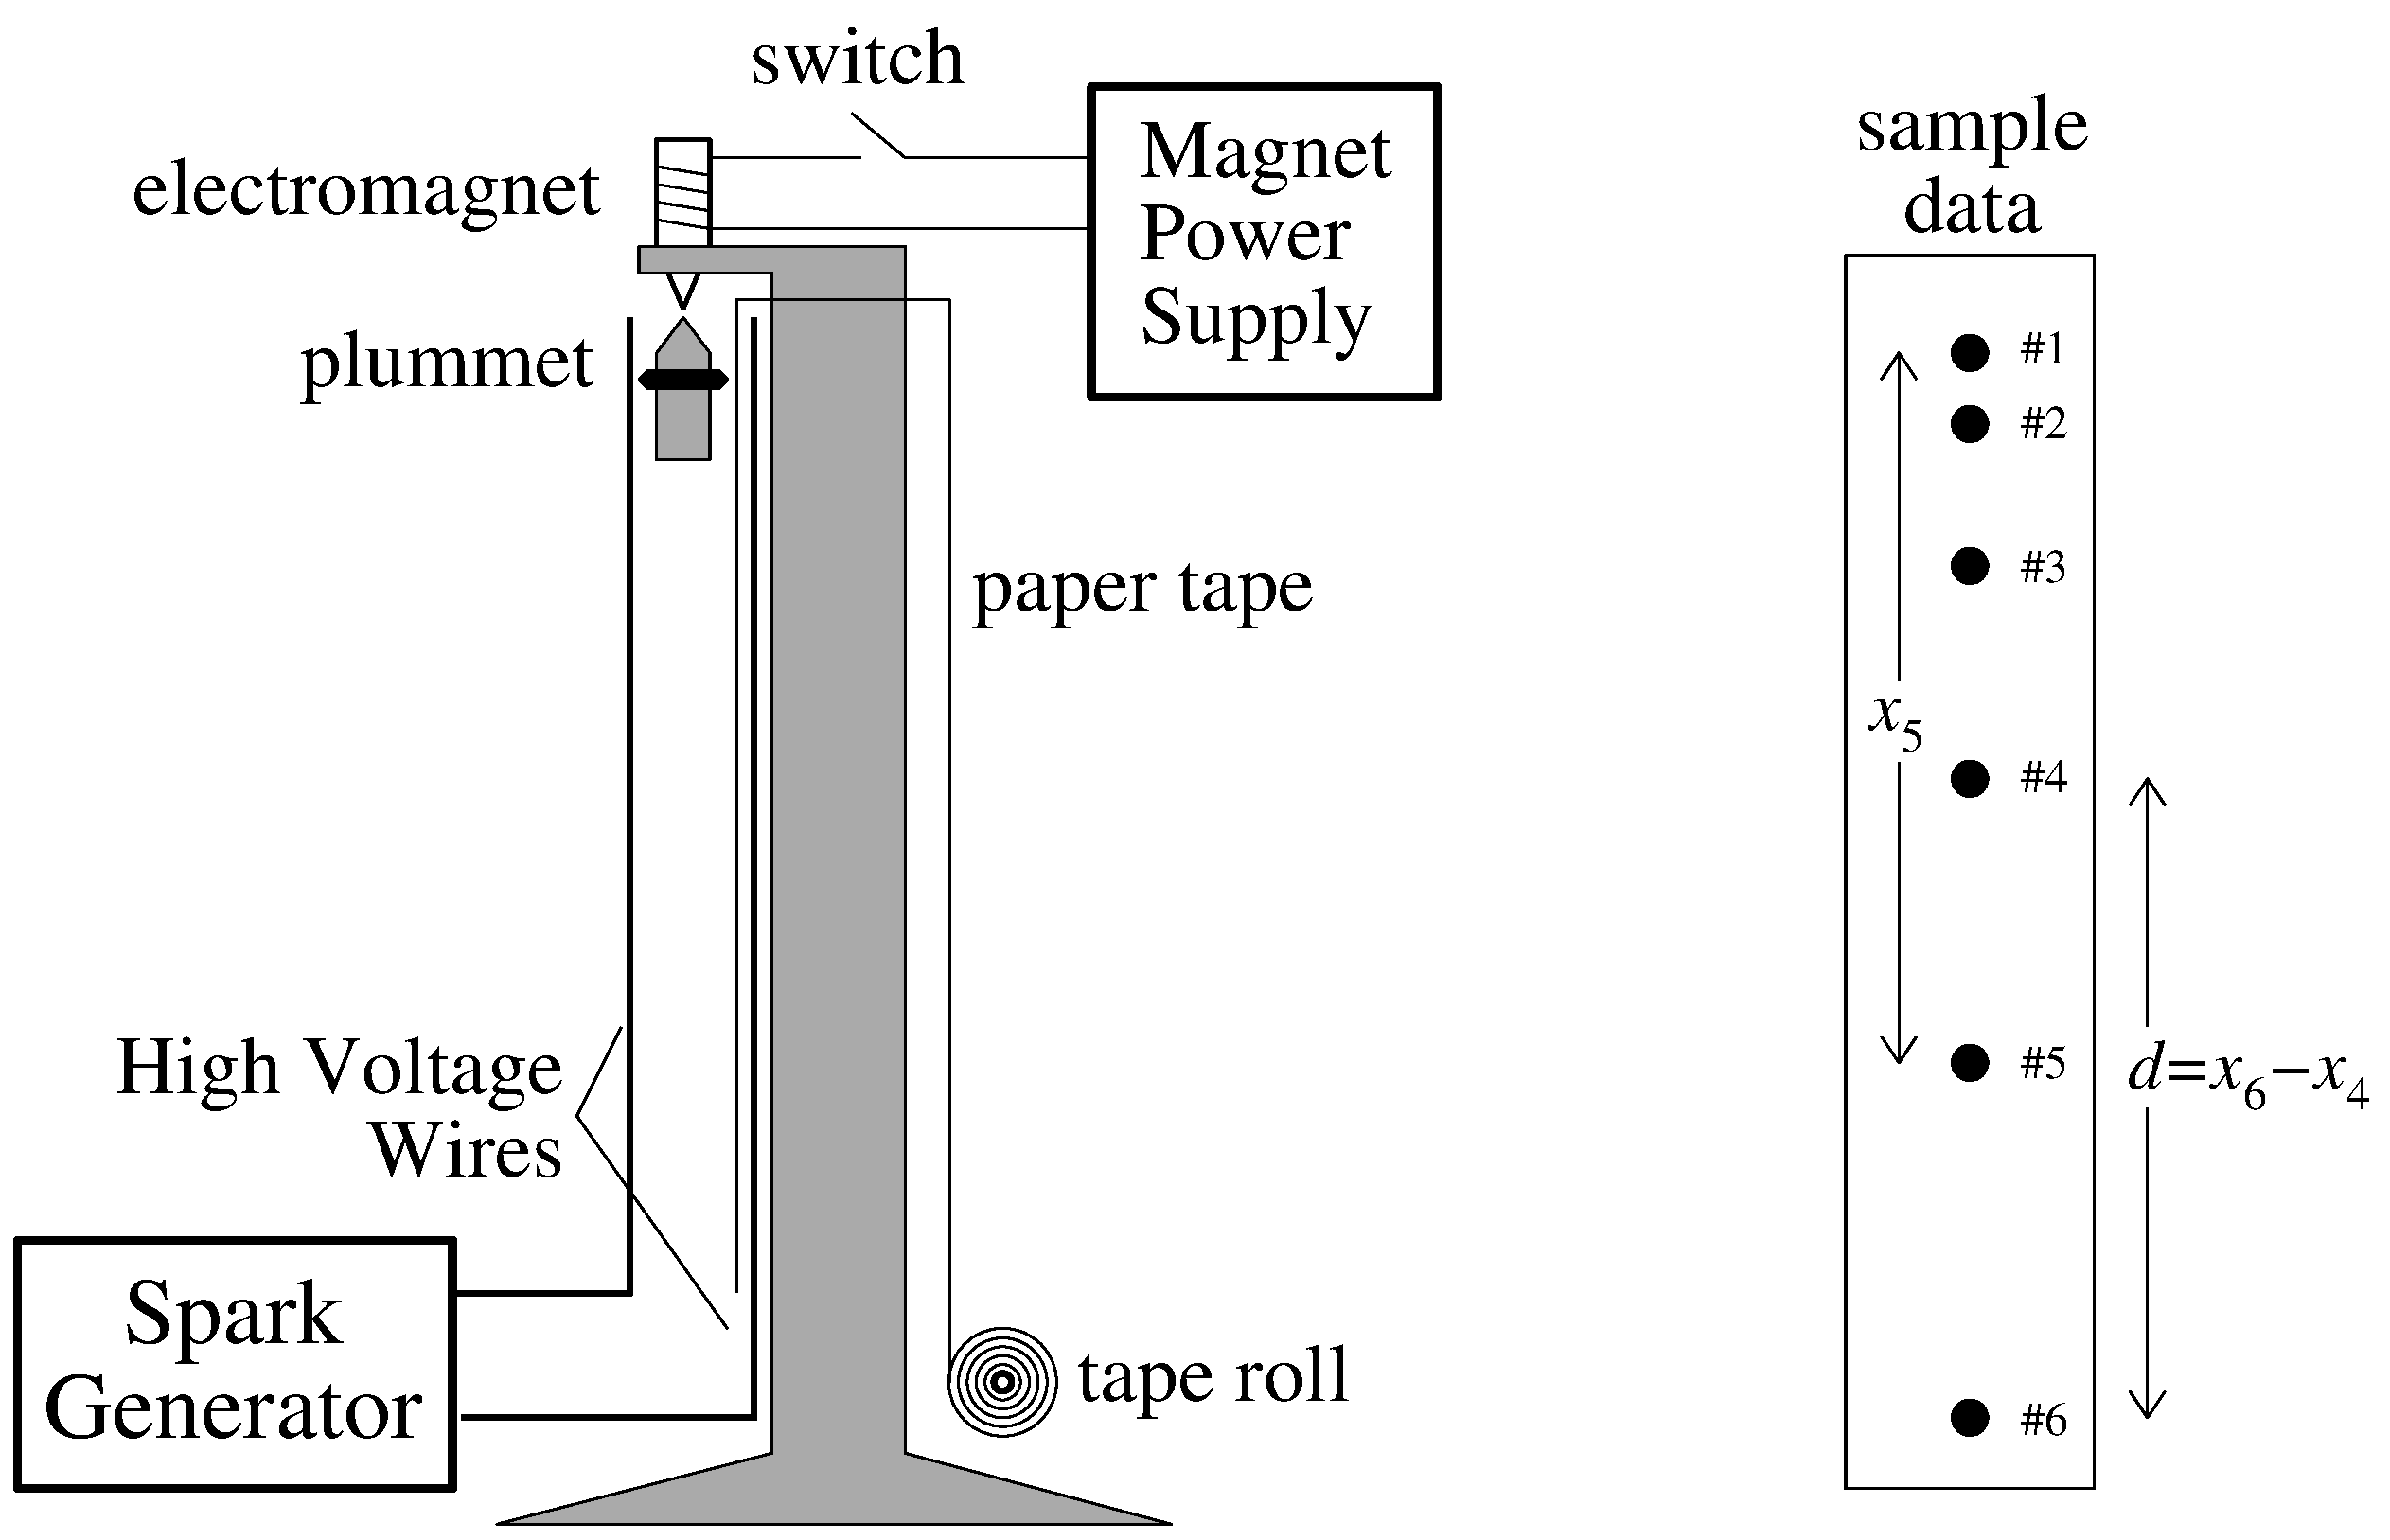
\includegraphics{behr2C.eps}}}}
\end{center}
%   \centerbmp{5in}{3.1in}{behr2.bmp}
 \caption{Behr Free Fall apparatus with sample data.  \label{fig:behr}}
\end{figure}
Check everything out with the instructor before using it.  When the switch to
the electromagnet is opened the plummet will fall freely.  The sparking system
will produce a spark hole through the sensitive paper every 1/60 of a second.
Since the spark jumps from the plummet to a wire behind the paper each spark hole marks
the position of the plummet at each spark time.  The resulting paper tape is thus a
record of distance fallen versus time.

%write and insert Appendix discussing Mean Speed Theorem
What about velocity as a function of time?  The instantaneous velocity is not
directly recorded on the paper tape.  Fig.~\ref{fig:behr} also shows a typical
section of tape with the dots representing spark holes at equal time intervals.
Using the Mean Speed Theorem, it can be shown that when the
acceleration is constant the instantaneous velocity at time $t_{5}$ is
numerically equal to the average velocity over the time interval $t_{4}$ to
$t_{6}$.  Hence from the information on the tape the velocity at time $t_{5}$
can be calculated by
\[
v(t_{5}) = {{d} \over {t_{6} - t_{4}}} = {x_6-x_4 \over t_{6} - t_{4}}
\]
We can use this trick for any combination of three successive dots on the tape
and thus determine the velocity as a function of time.

{\bf NOTE:} The choice of appropriate units for time can save you
a great deal of tedious computation. You will measure time
in units 1/60 sec, which we call a {\em wink} and velocity
 in units of cm per wink. Accelerations will come out in
cm/${\rm wink}^2$. After
you have completed the graphical and computer analysis and found
values for $g$, you can do a single unit conversion to
convert time back to seconds.  Ask your instructor or your TA if you
are not clear how to proceed.

\section*{Basic Procedure}
\begin{enumerate}\setcounter{enumi}{-1}
\item Read through {\em all} of this basic procedure and the following sections
on Uncertainties and Spreadsheet before beginning any measurements.

\item Ask the instructor to explain the operation of the apparatus to you.  Be
sure the apparatus is level, so the plummet will drop into the cup, and not hit
the wires on the way down.  Also, be sure you know how to operate the sparking
system without shocking yourself!

%If you think the apparatus is not level, ask {\em your TA} to level it
%for you.

\item Before installing the sensitive paper tape, make one or two trial runs
(Does the plummet drop without hitting wires?  Can you see sparks all the
way down the wires?  Don't touch the apparatus while the spark is on.)

\item Install the paper tape and take a final run to obtain data.

\item Remove the paper tape and check it immediately to see if all spark holes
are present (rerun if necessary).

\item Circle the spark holes and number them for convenience in making
measurements.

\item Decide what measurements you will make (see following on Uncertainties) and plan a data table 
accordingly.

\item Measure distances in cm.
Also, estimate the uncertainty in your
measurements of distance. (This uncertainty, $\delta x$, is probably the
same for every data point.)  Record the times, distances, and
uncertainties in the distances in a neatly constructed table.
%
\item Using your data, calculate velocity as a function
of time and enter the values
into your data table.  {\bf Note:}  You can calculate
the velocities with a calculator, but many people find it easier to use a
spreadsheet program---see below for detailed instructions.  
Also calculate the error in velocity.

\item  Analyze the $v(t)$ vs.\ $t$ data.  (A linear relationship is expected.)
Note: jumps in the $v(t)$ vs.\ $t$ graph usually indicate a missed spark hole.

\item Analyze the $x(t)$ vs.\ $t$ data.  (A quadratic relationship is expected.)

%\item Use the graph of $v(t)$ vs.\ $t$ to make a preliminary test of
%experimental validity---that is, see if all of your points appear to
%lie on a straight line.  It is easy to make an error in the
%calculations, but such errors will usually stand out prominently on
%a graph.  You are welcome to use Linfit to make the graph for this
%step.

%\item Do as much more of the data reduction and analysis as you have time
%for---it can be a help to do some of this work while help is available if
%needed.  Have the TA
%approve and initial your data before you leave.
\end{enumerate}

\section*{Uncertainties}

The uncertainties in this lab depends on the method
you use to reduce and analyze the data.  Two possibilities are listed below:
\begin{itemize}
\item[a.]  With the meter stick held firmly in place and {\em not}
zeroed on any particular spark hole, measure
the location $x$ of each spark hole.  Record the uncertainty  $\delta x$ of that
measurement. Note
that you will {\em not} want to use the first few marks on the
tape---they are usually  poorly defined.

Then, to find the velocities in units of
$\rm{cm}/{\rm wink}$, \underline{calculate}
the distances between every other point
using the individual $x$ values (e.g., $d_{4} = x_{5} - x_{3}$)
and then divide by 2 winks. (Why?)
%        If you use these units initially, you do not need to divide by
%        the time difference---see the explanatory note above.
	
In this case each individual value for $d$ has an uncertainty of
$\delta d = \sqrt{2} \cdot \delta x$.  Do you see why?  (Explain
this point in your writeup. Hint: see Eq.~E.5.) Divide $\delta d$ by 2 to get the uncertainty
in $v$. (Explain this point in your writeup. Hint: see Eq.~E.2.)

%{\em This method is strongly preferred.}

\item[b.]  Find the velocity directly by \underline{measuring}
the distance between every other point in addition to measuring
the location of each spark hole.
This method would give velocities with a bit better accuracy than the
first method, but would take twice as much time.
%give much less accurate results for the
%distance as a function of time, particularly for the data points
%towards the end of the tape.

%The reason is as follows: For each point, the distance from some
%starting
%point $x_0$ would have to be calculated from the measured $d$ values.
%Each of those values would have an error, so that the more values
%being added to find a given $x_i$, the larger the uncertainty for that
%point.  It is surprising but true that the method of reducing the data
%can affect the accuracy of the experiment!!

% 	\item[c.]  Measure the distance between each adjacent
% pair of points, picking
% up the meter stick each time and aligning it on the first point.  This
% method might seem reasonable, but in fact leads to much larger
% experimental errors.
%
%Let's call these measurements you made between points $p \pm \delta
%p$.  If you find a total distance $x$ travelled from the starting
%point, then each distance you measured must be added to the last
%total.  For example, the distance to the fourth point would be $x_4
%~=~
%p_1 + p_2 + p_3 + p_4$. That
%means that for each value of $x$ that you report,  the uncertainty
%will increase by $\delta p$.  Using the same example, $\delta x_4 ~=
%\delta p_1 + \delta p_2 + \delta p_3 + \delta p_4$.  As you can see, the
%uncertainty in the distance $x$ would be very large by the end of
%the tape!

\end{itemize}
Using either method will probably result in the same uncertainty
for every data point.  As a result \WAPP can calculate your
errors using a ``formula" (really just a constant), rather than using
individually determined errors for each datum.

%In each case you might choose a different value of raw data error.  In
%case a.  you probably listed a value for $\delta x$ of   %roughly $\pm~$0.5 mm.
%a few tenths of a millimeter.  In cases b.  and c.  you must deal with
%uncertainty
%at {\em both} ends of the meter stick, which should result in a larger
%uncertainty value.  It's your decision, so estimate the value that you
%think is prudent, and then later on you can check the accuracy of your
%estimate by scrutinizing the reduced chi-squared value in your fit
%results.

It turns out that in this experiment, the uncertainties in the time
$t$
are negligible compared to the uncertainties in the distance.
Otherwise, it would have been necessary to include both in calculating
the uncertainties in velocity, using the techniques developed in
Appendix A.

%After you find the velocities $v$, you must also find the
%uncertainties in those velocities
% $\delta v$. Recall that the calculated velocity
%\[
%	v ~=~  \frac{d}{\Delta t} = d
%\]
%
%         where $\Delta t$ is the time increment.
%        Thus  $\delta v ~=~ v \sqrt{(\frac{\delta d}{d})^2+(\frac{\delta \Delta t}{\Delta t})^2}$.  Explain this, referring to the rules in the appendix. Now find the equation for the resulting $\delta v$ if you assume that the error in time is negligible.
%
%Other error quantities can be calculated using similar methods. Once you know which things
%were measured, and their accuracy, simply
%use the rules for uncertainty propagation. A spreadsheet
%(as described in the following section) can save a lot of time in these sorts of calculations.


\section*{Using a Spreadsheet}

%This method will allow one to do most of the initial data reduction for
%the free fall experiment using the spreadsheet module in Linfit.  The
%following directions should also work with Microsoft Excel.  It should
%be possible to do more or less the same thing in other spreadsheet
%programs, although the exact sequence of commands may be slightly
%different.

\begin{enumerate}

\item Prepare a table of distances (in cm)
versus time (in units of winks).  Your times will fill the first column
and can be just the numbers
of the points: 1,2,3,\ldots . Your
distances (in the adjacent column) are the locations of the corresponding
spark holes.

%\item Enter these values into adjacent columns of the spreadsheet, with
%the times on the left and the distances on the right.  Then, save the
%spreadsheet, using whatever name you like.   You now have the data you
%will need to do your graphical and
%least-squares analysis of distance vs.\ time.

\item  Next, we use the
spreadsheet to calculate the velocities.  Follow these steps:
%
\begin{itemize}
\item  Put the cursor in the column to the right of the distances,
and click in the second row from the top (that is, the row corresponding
to $t=2$, the second data point).  Our aim is to calculate the
velocity at  that time: $v_2$.

\item  Next, enter a formula that will calculate the velocities.
First, type  ``{\tt =(}"  in the cell (without the quotation marks).

\item  Then, click on the distance cell diagonally down and to the
left (i.e., $x_3$).  If you are in the second row, this cell will be in the third
row.  You will see the cell reference in your formula.

\item  Next, enter a minus sign.

\item  Next, click on the distance cell diagonally up and to the left (i.e., $x_1$).

\item  Next, finish the formula that will calculate the velocities by
typing  ``{\tt )/2}"  in the cell (without the quotation marks).
You should see something like this:

{\tt =(B3-B1)/2}

\item  Hit Enter to finish the formula.  You should now have the
distance between the points immediately above and below your current
point divided by two---which is equivalent to velocity in units of 
distance per wink. Why?

\end{itemize}

\item  We now need to copy this {\em formula} to do the rest of the cells in
this column.  Select this cell again; notice the very small square
in the lower right hand side of the cell.  Click on that square
and drag it down.   This step should copy your formula to each cell
in the column and give
you the distance differences for all points except the first and last.

%Note that this column gives you the velocities in units of cm or
%mm
%per wink.  You can reduce the units of time to seconds if you want
%to.  But there is no need to do so.  Instead, you can do a single unit
%conversion at the end of your an analysis, after you have found $g$.

{\bf Be sure to include a sample calculation in your notebook, and
explain the reasoning behind it carefully.}  Your instructor should explain
a simple way to ``self-document" your spreadsheet before you print it.

\item  Save your spreadsheet, and print it.  You can tape it into
your lab book.  Be sure you label the columns appropriately 
(quantity name and unit) and 
document your procedure.

\end{enumerate}

\section*{Analysis of Data}

At this point you can transfer the data for velocity vs.\ time to \WAPP  and do your least-squares
fits.  Tell \WAPP that you have no $x$ errors (error in
time is ``negligible") and that you'll use a formula for $y$ errors
(really just a constant).  Click on ``Do Bulk".

Select (and copy) all three columns in your spreadsheet
(but not the first and last rows as  they lack corresponding velocities).
Paste that
data into the ``Block Copy \& Paste" web-form.  Enter the appropriate
$y$-error in the labeled box.  
When analyzing velocity vs.\ time
data the columns should be (respectively): X, Ignore, Y.
Click on ``Submit Data". Print out a copy of the resulting fit report after
examining the velocity vs.\ time plot.
The points should all lie
close to a straight line.  If they do not, you may have recorded some points from your
tape incorrectly---double-check, and consult your instructor if necessary


When analyzing distance vs.\ time copy and paste all of the rows
(but only the two required columns);
the columns should be (respectively): X, Y. 

%Select the data and use the Data/Move Selection to Data Screen
%menu item to transfer the data.
%Note that the data you select do not have to be in adjoining columns.
%Select the data in your first column, and then hold the Control key
%down while you select the data in the second column.  Please see
%Appendix D for a more complete discussion.

%It is not a bad idea to save the spreadsheet at this
%point if you have not already done so.

%Now that you've done some calculations, you can begin to try
%things on your own.  For example, the column for the
%uncertainties in the velocities  can easily be generated by putting
%in the formulas found in the
%discussion above.

The main purpose of this experiment is to measure the acceleration of
gravity $g$ (of course, with an experimental uncertainty $\delta g$).  We will
find $g\pm\delta g$ using {\bf two separate methods}, and see how well the two compare.

%For this analysis, you may need to review Appendices A, C and D in
%the  back of the lab manual (see
%pages~\pageref{datanal}~and~\pageref{compassis}).

{\bf METHOD 1: }
Study velocity as a function of time with a
fit/graph of \underline{velocity} (on the $y$-axis) vs.\ time (on the
$x$-axis).  According to Eq.~\ref{eq:v(t)}, velocity should be
a straight line function of time, with slope $g$.  Fit and plot your
$\{(t,v)\}$ data using a linear function; \WAPP should
report the slope, $B$, with an uncertainty.  The units of that slope are
${\rm cm/wink}^2$.  (Explain why in your notebook.) Using
$60\mbox{ wink}=1\mbox{ second}$, unit-convert that slope 
(and its uncertainty) to cm/sec$^2$.
Be sure that you record all these calculations carefully in your lab
notebook.
Also, report your value for reduced chi-squared
and comment on its significance. 

%Using your graph,
%find the slope (which is $g$), convert it to units of m/sec$^2$ or
%cm/sec$^2$.  Estimate the uncertainty in $g$ from the same graph.  {\bf
%Hint:}  If you are not sure how to proceed, look up the theoretical
%result for velocity as a function of time in a constant gravitational
%field.

%Be sure that you record all these calculations carefully in your lab
%notebook.

%Then repeat this analysis by doing a least-squares fit with Linfit.
%Again, use the result of the least-squares fit to report $g$ and the
%uncertainty in $g$.  

{\bf METHOD 2: }
Study position as a function of time with a
fit/graph of \underline{distance} ($y$-axis) vs.\ time ($x$-axis).  
According to Eq.~\ref{eq:x(t)}, there should be a quadratic relationship
between $x$ and $t$.   Do a least squares
fit.  Each of the parameters in the fit ($A$, $B$, and $C$) correspond to
a term in Eq.~\ref{eq:x(t)}.  Unit convert each one of these terms to
normal units and use the results to report values (with error) for
$x_{\circ}$,   $v_{\circ}$, and $g$.
Again, report your value
for reduced chi-squared and comment on its significance. Tape the
fit report and graph into your notebook.



\section*{Conclusions}
Summarize your results by making a careful table in your lab book that
reports $g$ and the uncertainty in $g$ using the two methods. % (graphical
%and least-squares fit) employed above.  
Be sure you report these
results using time in units of seconds.

Then, compare (see page~\pageref{scierror}) your experimental values
for $g$
with the value 980 cm/s$^{2}$ usually given in textbooks as the
accepted value.

In your conclusion, give a careful discussion of your results.
For example, how reliable are the least-squares fits and your
estimates of experimental uncertainty, given your reduced chi-squared
values?
Comment on the consistency of your results and how well they compare to the
accepted value (give a percent difference).  Mention any sources of error, both
systematic and random.


\section*{Critique of Lab}
Follow the suggestions given in the Introduction to the
Laboratory Manual.

\section*{Quick Report Card}
Properly report (sigfigs, error, units) your two values of $g$.

\section*{Extra Credit}
Make an additional column of $v^2$ data.  Test the relationship between
velocity squared and position:
\begin{equation}
v^2=(v_o^2-2gx_o)+2gx
\end{equation}
Use Eq.~E.4 to find the formula for the error in $v^2$.  From the slope
of the $v^2$ vs.\ $x$ relationship, find $g$ a third way.


\renewcommand{\newname}{Reaction Time and Falling Bodies}
%REACTION TIME AND FALLING BODIES
\newexp
{\bf Note:} We will not be doing this experiment this year.
Nevertheless, no special equipment is required and you are encouraged
to try this lab on your own.

\begin{tabbing}
reference12345 \= col2 \kill
References: \> {\em An Introduction to Error Analysis}, John R.\ Taylor,
   chapters 4, 5.  We strongly \\
\> recommend this book for students majoring in pre-engineering or
the physical \\
\> sciences. \\
\end{tabbing}

\section*{Before Lab}
This experiment relies heavily on the material developed in Appendix A
of this lab manual---Please review it carefully.  And of course, study
this writeup carefully.

\section*{Introduction}
     In this experiment we will measure the reaction times of the
experimenters as a way of examining the random scatter in
experimental data.  We will also introduce the {\em standard deviation}
 as a measure of
that scatter.  Keep in mind that experimental scientists
distinguish between random error and systematic error; we will be
concerned only with the former in this experiment.  See Taylor
and Appendix A in the lab manual (p.~\pageref{scierror})
for a more complete discussion.

\section*{Analysis of Problem}
      One normally thinks of measuring a given physical
quantity with a particular instrument.  For example, one
ordinarily measures length or distance with a meter stick, time
with a clock, mass with a balance, and so on.  In this exercise,
however, we will see how one can measure reaction time with a
meter stick.  We will also study the random variations in the
data and the way one can estimate the ``best" value of the
reaction time.

We can find a person's reaction time by measuring the distance fallen
by a meterstick and using the law of falling bodies to calculate the
time it has taken to fall that distance.  If we let $D$ represent the
distance, $t$ the time, and $g$ the acceleration of gravity, then
\begin{equation}
D = {{1} \over {2}} \: g t^{2}  \label{eq:react1}
\end{equation}
We will solve this equation for time to find time as a function
of distance fallen.

\section*{Experimental Procedure}
     Two people working together can measure their reaction times
as follows:  One person holds a meter stick by its upper end.
The second person, whose reaction time is to be measured, places
one or both hands lower on the stick, in a position that can be
reproduced from one measurement to the next.  Without warning,
the first person drops the stick.  The second person closes his
or her hand so as to grab the stick.  Then s/he records the
distance the stick fell. This procedure should be repeated 40
times, maintaining the experimental conditions as nearly alike as
possible for all the measurements.  {\bf PLEASE NOTE:}  You should work
out your procedure carefully and describe it {\em in detail} in your
laboratory notebook before you take your measurements.  For
example, how did you make sure your hand didn't move up or down
as you grabbed the meter stick?  What other potential problems
did you consider?   And so on---be complete in describing your procedure.

     In formulating your procedure, you should also consider how
accurate your measurements will be, and what steps you might make
to improve that accuracy.  Even though these will not be
measurements of high precision, you should be able to measure
each distance to better than one centimeter.  However, one can
hardly expect to be as accurate as
one millimeter, at least without much fancier apparatus.
You should also estimate how accurate your times
will be, given the accuracy with which you can measure distance.

\section*{Reduction and Analysis of Data}
     Note that, even with care, successive measurements will not
give exactly the same result. This situation arises in making and
analyzing measurements of all sorts and will be the focus of our
analysis in this experiment.

     We must begin by converting all our distances into reaction
times, using Equation~\ref{eq:react1}.  (Note that we cannot find the average
reaction time simply by averaging the distances and converting
the average distance into an average time, since the average of
the squares of a series of numbers is not equal to the square of their
average.  Note for example that for the two numbers 3 and 5, the
average of their squares, 17, is not the same as the square of
their average, 16.  This example shows that one needs to convert
all of the measured distances into the corresponding times.)

     The conversion from the measured distances to the
corresponding times can be calculated using Equation~\ref{eq:react1}.
One can use a calculator, but you may also use a spreadsheet such as
the one in Linfit to do these calculations if you prefer.

     Record your calculated reaction times and your estimate of
their uncertainties in a data table.  You are now ready to start
the data analysis.

     When an experimental quantity --- time, in this case --- is
measured several times the results obtained are often influenced
by a number of factors that fluctuate in an independent and random
fashion.
(What are some of those factors in this experiment?)  Some of the
factors may make the measurement appear larger and some smaller.
Usually, most of the measurements will lie near
the center of the observed range rather than be very large or
very small compared with the average.  To learn very much from a
series of measurements of a quantity, one needs to decide what is
the ``best" value of the quantity and also to obtain a number
which describes the range of variation on either side of the
``best" value.

     If the experimental conditions do not change during a series of
measurements, the ``best" value of the result is usually the
average or mean.  To obtain your average reaction time, add
together the individual times and divide by the total number:
\begin{equation}
\mbox{average time} = A = {{(t_{1} + t_{2} + \cdots + t_{N})} \over {N}}
   \label{eq:react2}
\end{equation}
where $A$ is the average time and $N$ is the number of measurements.

     To describe the data more completely, one
needs to specify the range or spread that characterized the data.  One
might simply specify the lowest and highest values observed; but this
procedure is often misleading because very often one point will
be much higher or much lower than any other.  A more common way
of describing the spread of results is to give a number which,
when added to or subtracted from the average result, will give
values which include about 2/3 of all the measurements.  This
number describing the spread of results is called the {\em standard
deviation} of the measurement and is usually designated by $\sigma$
(the lower case Greek letter sigma.

\paragraph*{Determination of Standard Deviation from Experimental Data}

     We begin with the definition of the deviation.  For the $i$th
data point, the deviation $d_{i}$ is defined as
\begin{equation}
d_{i} = t_{i} - A  \label{eq:react3}
\end{equation}
Intuitively, the sum of the absolute value of deviations divided by the number of
measurements  should provide a reasonable
measure of the scatter in the data.  This quantity is called the
average deviation---see Appendix A.

However,
a more rigorous and widely used measure
turns out to be the standard deviation $\sigma$, defined as
\begin{equation}
\sigma = \sqrt { {{1} \over {N - 1}} \: \sum_{i} \, d_{i}^{2} }
  \label{eq:react4}
\end{equation}
It can be shown that under most circumstances, about 2/3 of the
observations should lie within one standard deviation of the
average value.

     We will employ a graphical procedure to investigate this
claim.  First, along a line, lay out a scale that will cover the
range of measurements in the whole group.  Then make a mark on
the scale to represent each one of the measurements, as shown in
Fig.~\ref{fig:react1}.  If two or more of the measurements result in exactly
the same value, make one mark above the other so both can be recorded
as being on that point of the line.  Next, determine the average
value of all the measurements and mark that point on the line as
point $A$.  Count the number of points along the line that
correspond to values of the measurement smaller than $A$ and mark
the point ($A - \sigma$) which divides this group so that about 2/3 of the
points below $A$ are are between $A$ and ($A - \sigma$).
\begin{figure}
\begin{center}
{\resizebox{5.1in}{!}{{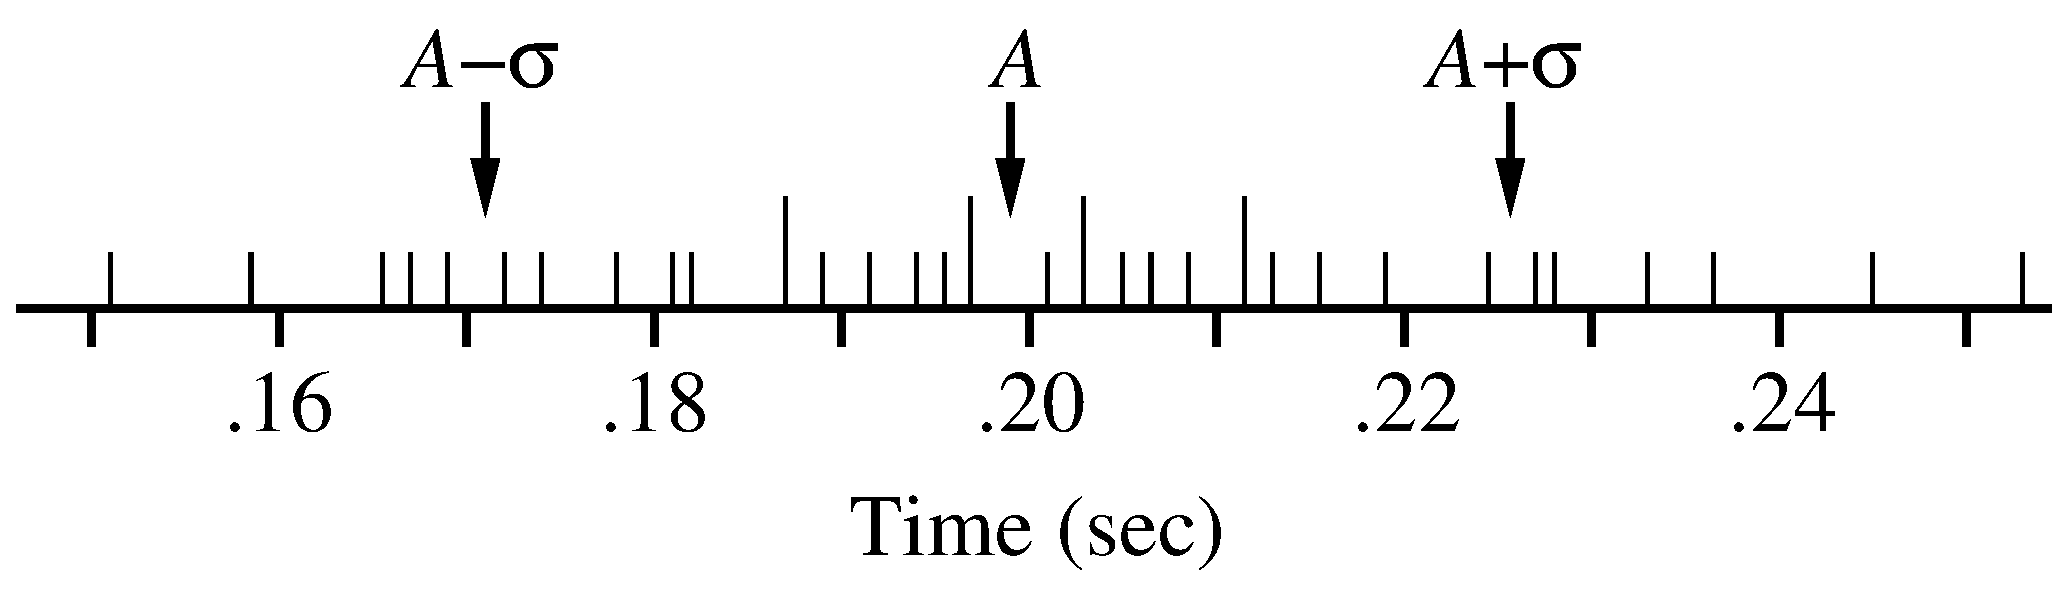
\includegraphics{reactionC.eps}}}}
\end{center}
%\vspace{0.75in}
% \centerbmp{5.1in}{.86in}{reaction.bmp}
 \caption{Sample distribution diagram of reaction time data.   \label{fig:react1}}
\end{figure}
Mark the point ($A + \sigma$) which divides the points above $A$ so that
about 2/3 of them are between $A$ and ($A + \sigma$).

     If the distribution of points about the average value is
symmetric, the distance along the scale from $A$ to ($A - \sigma$) will
equal the distance along the scale from $A$ to ($A + \sigma$), and this
distance $\sigma$ will be the standard deviation of this set of
measurements.  Thus we can say that about two measurements in
three will lie in the range ($A \pm \sigma$).

     If the distance from $A$ to ($A - \sigma$) is slightly different from
the distance from $A$ to ($A + \sigma$), one can obtain an approximate value
for the standard deviation by taking half the distance from ($A - \sigma$)
to ($A + \sigma$).  If these two distances are greatly different, the
concept of standard deviation may not applicable to the set of
data.  In this asymmetric case one should give the spreads of the
data in both the upward and the downward direction which include
2/3 of the points on either side in the form
\[
A^{+U}_{-L}
\]
     Still a third indication of the spread of a set of data is
called the ``probable error", which includes one half of all the
measurements within its limits.  When writing a result as ($A \pm B$)
one should identify which measure of the spread is being used.
The standard deviation, which is easily calculated on a computer
and on many pocket calculators, is the most commonly used
measure.

\paragraph*{Normal Distribution of Errors}

     To aid one in understanding the fluctuations in the results
of a measurement it is often helpful to draw a bar-graph or
histogram similar to the one shown in Fig.~\ref{fig:react2}.  In drawing this
graph one needs to divide the points plotted in Fig.~\ref{fig:react1} into
groups which are broad enough to smooth out the major
fluctuations but are not so wide as to mask the general trends.
\begin{figure}
\begin{center}
{\resizebox{5in}{!}{\rotatebox{-90}{\includegraphics{fig3.2.ps}}}}
\end{center}
% \vspace{3.25in}
% \hspace{.5in}
% \special{bmp:bgphnorm.bmp x=4.79in y=3.25in}
\caption{Bar graph (normal distribution).  \label{fig:react2}}
\end{figure}
\begin{figure}
\begin{center}
{\resizebox{5in}{!}{\rotatebox{-90}{\includegraphics{fig3.3.ps}}}}
\end{center}
% \vspace{2in}
% \hspace{1in}
% \special{bmp:bgphnon.bmp x=4.12in y=2in}
 \caption{Bar graph (non-normal distribution).  \label{fig:react3}}
\end{figure}
     In an ideal or normal distribution of random errors this
graph has one peak and is symmetric about the average value.  In
some situations, where there is an unexpected change in the
quantity being measured, there may be two peaks, as shown in
Fig.~\ref{fig:react3}.  In the other cases the distribution will extend much
further on one side of the average than on the other.  In case of
such non-normal distributions one should not try to represent the
results by a single average and standard deviation.

\paragraph*{Standard Deviation of the Mean}

     The standard deviation is a measure of the average
uncertainty of {\em an individual data point} --- that is, if we know the
standard deviation $\sigma$ and the average $A$, we know that the chances
are about 2 in 3 that any {\em single} point will lie in the range
$A \pm \sigma$.

But it is reasonable to suppose that our knowledge of
the average value is more accurate (or less uncertain)
than our knowledge of any single data point.
     Indeed, this statement can be shown to be correct.  The
appropriate uncertainty in the {\em average value} of a set of
measurements is the {\em standard deviation of the mean}, defined as
\begin{equation}
S = {{\sigma} \over {\sqrt{N}}}  \label{eq:react5}
\end{equation}
where $N$ is the number of data points used in determining $\sigma$.

     If one takes more data points for a given measurement, the
spread in those points, described by $\sigma$,  probably will not
change much, but the accuracy of their average, described by $S$,
will improve as $N$ becomes larger.  {\bf PLEASE NOTE:}  In reporting a
measurement, always state explicitly whether you are citing a
standard deviation or a standard deviation of the mean.

Please see Appendix A for a more complete discussion.

\paragraph*{Analyzing your Reaction Time Data}

\begin{enumerate}
\item Divide your data into two groups, using the first 20 points as
   one group and the second 20 points as the other.
\item For each group separately make a data distribution diagram as
   shown in Fig.~\ref{fig:react1}.
\item Calculate the average value for each group, $A_{1}$ and $A_{2}$, and
   mark $A_{1}$ and $A_{2}$ on its diagram.
\item For each group mark on the diagram the points ($A + \sigma$) and
 ($A - \sigma$).
   Using the 2/3 criterion, determine the standard  deviations for
   each group and compare them with the values obtained using
   Equation~\ref{eq:react4}.  You may find it convenient to use
   a spreadsheet for these calculations.
%
\item Using Equation~\ref{eq:react5}, compute the Standard Deviation of the Mean
for each group.
\item Compare the results of your group 1 with the results of group 2.
   One can say the results are highly consistent if the absolute value of the
   difference
   between $A_{1}$ and $A_{2}$ is less than ($S_{1} + S_{2}$).
If $|A_{1} - A_{2}|$ is
   less than 2($S_{1} + S_{2}$), the results are moderately consistent.
   If $|A_{1} - A_{2}|$ is more than 2($S_{1} + S_{2}$), there may have been a
   trend in your response as you gained experience in grabbing the
   meter stick, or perhaps some other source of systematic error is present.
\item Compute $A$, $\sigma$, and $S$ for the whole set of data and compare your
    results with those of others in your class.  For this part use
    Equations~\ref{eq:react4}~and~\ref{eq:react5}.
%
\item Draw a distribution bar graph as shown in Fig.~\ref{fig:react2} for the
    whole set of data.  How well does it resemble a ``Normal" distribution?
\end{enumerate}

\section*{Conclusions}
Make a careful table listing all your numerical results and their
uncertainties, and give a careful discussion of them.
Comment on the consistency of your results and how they compare to the
results of others in your class.  Mention any sources of error, both
systematic and random.

\section*{Critique of Lab}
     Follow the suggestions given in the Introduction to the
Laboratory Manual.


\renewcommand{\newname}{Projectile Motion}
%PROJECTILE MOTION
\newexp

\section*{Before Lab}

BEFORE COMING TO LAB: Do some preliminary uncertainty analysis.  You
will be calculating the horizontal velocity $v_{x}$ of a
projectile from your measurements
of horizontal distance $x$ and vertical distance $y$, using
Eq.~(\ref{eq:vx}).  Read through the write-up and be sure you
understand the theory, and how the experiment works.

Since these measurements will
have uncertainties $\delta x$ and $\delta y$, there will be a
resulting
uncertainty $\delta v_{x}$ in the calculated velocity.  Work out an
expression for its {\em relative} uncertainty $\delta v_{x}/v_{x}$
in terms of the relative uncertainties of the measurements.  See Appendix
A for help.

 Get your TA to initial your preliminary uncertainty
analysis.


\section*{Introduction}
     Continuing the work of his Medieval predecessors, Richard Swineshead,
William Heytesbury, John Buridan, and John Dumbleton, Galileo was greatly
concerned with the science of motion: how one describes the behavior
of
moving bodies.  One of his particular interests was
projectile
motion. In his work {\em Two New Sciences}, he writes:
\begin{quote}
\begin{center}
On the Motion of Projectiles
\end{center}
We have considered properties existing in equable motion, and those in
naturally accelerated motion over inclined planes of whatever slope.  In
the studies on which I now enter, I shall try to present certain leading
essentials, and to establish them by firm demonstrations, bearing on a
moveable when its motion is compounded from two movements; that is, when it
is moved equably and is also naturally accelerated.  Of this kind appear to
be those which we speak of as projections, the origin of which I lay down
as follows.

I mentally conceive of some moveable projected on a horizontal plane, all
impediments being put aside.  Now it is evident from what has been said
elsewhere at greater length that equable motion on this plane would be
perpetual if the plane were of infinite extent, but if we assume it to be
ended, and [situated] on high, the moveable (which I conceive of as being
endowed with heaviness), driven to the end of this plane and going on
further, adds on to its previous equable and indelible motion that downward
tendency which it has from its own heaviness.  Thus there emerges a certain
motion, compounded from equable horizontal and from naturally accelerated
downward [motion], which I call ``projection."  We shall demonstrate some of
its properties [accidentia], of which the first is this:
\begin{center}
PROPOSITION I.  THEOREM I.
\end{center}
\begin{quote}
When a projectile is carried in motion compounded from equable horizontal
and from naturally accelerated downward [motions], it describes a
semiparabolic line in its movement.
\end{quote}
\end{quote}

Galileo had discovered a fascinating concept: The motion of
an object in the earth's gravity is accelerated downward with the same
acceleration {\em irrespective of its horizontal velocity}.
So if one neglects air resistance, an object dropped from 40 meters will
hit the ground at the same time
as a similar object launched horizontally from the same height.  One
can analyze the vertical motion separately from any horizontal
movement.

The purpose of this experiment is to investigate Galileo's conclusions
about projectile motion:  that it is compounded of two
independent motions---a horizontal component and a vertical
component---and that the path followed is parabolic.
%\section*{Video Lab}
%You and the the rest of the class will become camera jockeys in this lab by filming the
%motion of a projectile.  The TA will be helping you to set up and record
%a projectile flight clearly enough that you can take data from the frame-by-frame
%advance of the film.  This data will have bigger error than the experiment which follows,
%but is a great way for you to quickly see that the trajectory of a launched object is,
%indeed, parabolic.  Show this by fitting your rough $y$ vs $t$ via LINFIT (You can
%use the first half of flight if you wish). This is to be a class project.  In your final
%summary of this data, describe what you saw in the video in the x-direction and
%y-direction independently.  {\em Note: you can use units of Frames for the time
%and Bricks for the distance}

\section*{Experiment}

\begin{figure}[hbt]
\begin{center}
{\resizebox{5in}{!}{{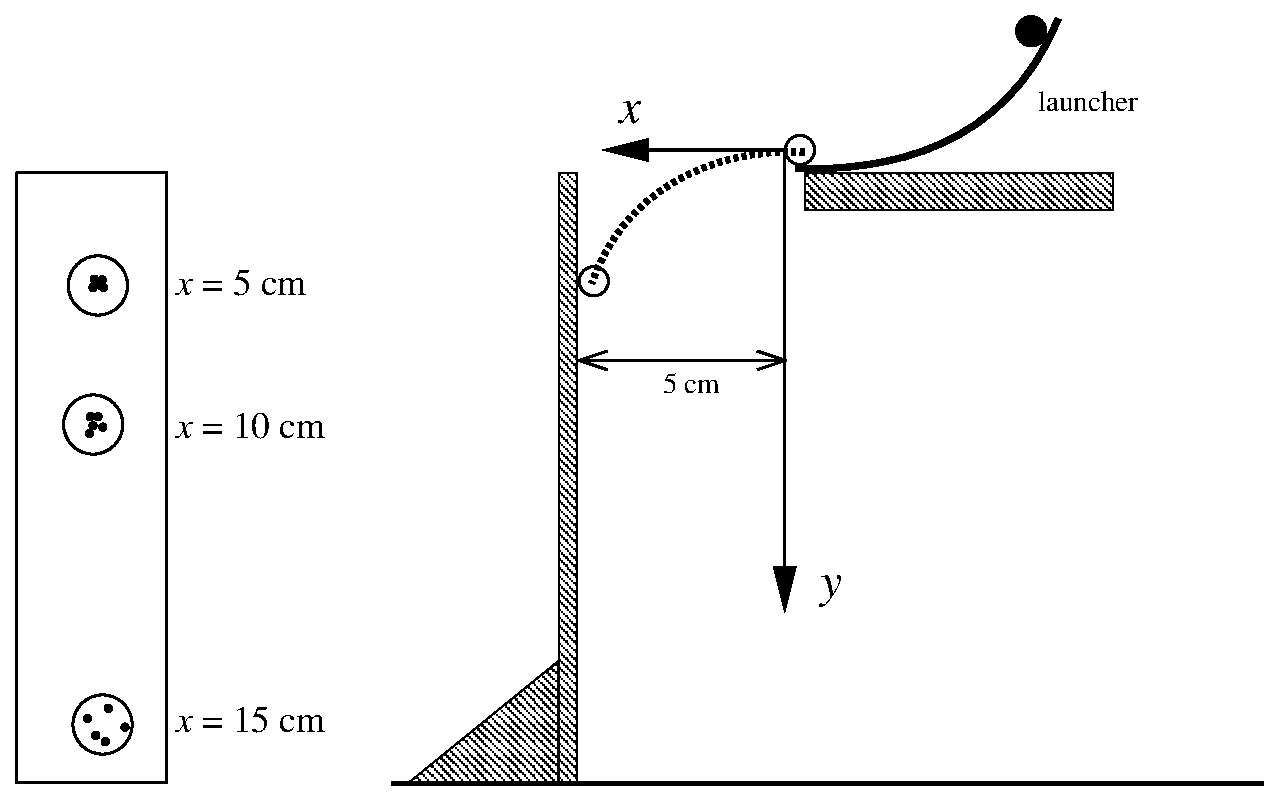
\includegraphics{projectile.app.eps}}}}
\end{center}
%\vspace{3in}
%\special{eps:projectile.app.eps x=5in y=3in}
%\special{wmf:figa1.wmf} % x=3.44in y=1.5in}
 \caption{Projectile motion apparatus.  \label{fig:projectile}}
\end{figure}
The apparatus for this experiment is simple, but can yield reasonably
good data if careful measurements are made.  You will be
launching steel ball bearings as projectiles.  A projectile launcher
will
get the ball moving and launch it horizontally (i.e., $v_{0y}=0$) from a table towards a
vertical board covered with carbon paper.
The carbon paper marks the ball's point of impact.
The horizontal distance $x$ traveled is changed by moving the board
further and further away. The vertical distance $y$ it falls
will be measured as a function of $x$.  The relationship between these distances determines
the shape of the ball's flight path.

The important equations should be familiar by now.  If the projectile has a
constant velocity $v_{x}$ in the $x$ direction, and is gravitationally accelerated in
the $y$ direction, then
\begin{eqnarray}
x & \!\!= &\!\! v_{x}t \\        \label{eq:xproj(t)}
y & \!\!= &\!\! \frac{1}{2}gt^{2} \label{eq:yproj(t)}
\end{eqnarray}
where $t$ is the time for the ball to fall a distance $y$ and move
a distance $x$ horizontally.
From Eq.~(\ref{eq:yproj(t)}) we see that the time of flight is
\begin{equation}
t = \sqrt{\frac{2y}{g}}  \label{eq:t(y)}
\end{equation}
so the horizontal velocity is
\begin{equation}
v_{x} = x/t =  x\sqrt{\frac{g}{2y}} \label{eq:vx}
\end{equation}
If we square both sides and solve for $y$, we obtain
\begin{equation}
y = \frac{g}{2v_{x}^{2}}x^{2}, \label{eq:y(x)}
\end{equation}
which is the equation of a parabola.  You will be testing whether $v_{x}$
does in fact remain constant, and whether the path is parabolic.

\section*{Procedure}
\begin{enumerate}

\item Attach paper to the board.  Use the launcher to make a horizontal line
on the paper representing $y = 0$.

Use a plumb line from the end of the launcher to set the $x = 0$ point on the
floor.  Notice that you will need to correct the horizontal distance $x$ for
the radius of the ball, and the launch position of the ball as it leaves the
launcher.  Check with your instructor if you are uncertain about this correction.  

%Note the inconvenient location of the origin:
%at the far edge of the ball --- a radius up in $y$ and a radius less in $x$ from the track end.
%The easiest solution is to use the track-end as the origin in recording data, and then
%adjust the $(x,y)$ locations all at once in the spreadsheet.  Make a horizontal line on the
%paper representing the height of the track surface and vertical line as an aim point for the
%balls.

\item  Attach carbon paper to the board, so that the ball will leave a mark where
it hits the board. 
Move the board 5 cm away from the end of the launcher (so that your first (uncorrected) 
horizontal distance is $x$ = 5 cm);
Estimate of the
uncertainty, $\delta x$, in the boards location. Use a level to check that the board is vertical. 
Now launch the ball and check that it
left a carbon mark on the paper where it hit the board.  Repeat four more times. 
%{\em Note: Observe all safety precautions in the lab!}

\item  Estimate the vertical distance
the ball traveled for an average trial.  Estimate the uncertainty $\delta y$ from the
half the spread in $y$.

\item  Continue these measurements for horizontal distances of 10, 15,\ldots
50 cm.  Make a table for your data and calculations something like this:

\begin{center}
\begin{tabular}{|c|c|c|c|c|c|}
\hline
$x$ & $\delta x$& $y$ & $\delta y$& $v_{x}$ & $\delta v_{x}$ \\
 (cm) & (cm)   &  (cm)& (cm)      & (cm/s) &  (cm/s)\\
\hline
 \phantom{10000}& \phantom{10000}   &  \phantom{10000}& \phantom{10000}      & \phantom{10000} &  \phantom{10000} \\
\hline
  &   &  &  &  &      \\ \hline
  &   &  &  &  &      \\ \hline
\end{tabular}
\end{center}
\item Calculate the velocities $v_{x}$ for the table.  Their uncertainties
should be easy to compute using the formula you worked out before coming to
lab.  Does $v_{x}$ appear to be constant, within the limits of your uncertainties?

%\item Make a graph of $y$ vs.\ $x$, including error bars to indicate the
%uncertainties, and sketch the curve as best you can.

\item  In this experiment, the errors in both $x$ and $y$ are
typically non-negligible, and so you will probably want to
include the uncertainty in $x$ in your least-squares fit in Linfit.

%Be sure to include the $x$ error bars on your graphs.

%There is a complication in using LINFIT this time.  Because of
%the nature of the numerical algorithm generally used for least-squares
%fits, LINFIT will only accept uncertainties in $y$, and not in $x$.
%But your data probably has significant errors in both $y$ and $x$.
%One way to deal with this problem is to transform the uncertainties in
%$x$ into additional uncertainties in $y$.
%
%Graphically, this scheme is not hard to follow.  Examine your graph of
%$y$ vs. $x$, and note that an uncertainty in $x$---a horizontal error
%bar---has the same effect as a proportionally {\em larger} $y$ error
%bar.  Be sure you understand this point qualitatively.
%
%The mathematics requires a little bit of calculus.  We begin
%by rewriting Eq.~(\ref{eq:y(x)}):
%
%\[
%y = \frac{g}{2v_{x}^{2}}x^{2}
%\]
%
%Next, take the derivative of $y$ with respect to $x$:
%\[
%{dy \over dx} = {g \over {v_{x}^2}} x  = {2y \over x}
%\]
%where the result on the right follows by substitution---take a few
%minutes and be sure you understand how the calculation works.
%
%If we convert this result from a derivative to a differential, we
%obtain
%
%\[
%\delta y = 2y {\delta x \over x}
%\]
%In this form, we have an equation that gives the uncertainty in $y$
%due to a corresponding uncertainty in $x$.  The total uncertainty in
%$y$, then, is this result added to the experimental uncertainty in
%$y$.  If we call this total uncertainty $\delta y'$, we have
%
% \begin{displaymath}
%  \delta y' =  \delta y + 2 y \frac{\delta x}{x}
%\end{displaymath}
%as the uncertainty.  Compute a list of these ``corrected"
%uncertainties to go with your $y$ data.  It may be convenient to
%use a spreadsheet for these calculations.

\item Use LINFIT to test whether $y(x)$ is a parabola; fit the data using
the form $Y = AX^{B}$, where $B$ is not a fixed constant, but a variable to
be determined by LINFIT.  Compare your values for the parameters $A$ and $B$
to the predictions of Eq.~(\ref{eq:y(x)}).  $B$ ought to be somewhere near
2, and $A$ should be approximately $g/(2v_{x}^{2})$.
Make normal and log-log plots of your results.

\item A better value for $A$ is obtained if we fit 
to $Y = AX^{B}$ but keep $B$ constant
at 2.  Due to Linfit limitations, this will require turning off
$x$ errors.  Calculate $v_x$ from this $A$ value.

\section*{Conclusions}

Discuss the results of the experiment:  Is the horizontal component of
velocity constant, within experimental uncertainty?  And are your data
consistent with a parabolic path?  As always, give detailed analysis
of your least-squares fits, including a discussion of the reduced
chi-squared value.

\section*{Critique of Lab}
     Follow the suggestions given in the Introduction to the
Laboratory Manual.




\end{enumerate}
\newpage
%\cleardoublepage
%\begin{center}
% CHECKLIST FOR PROJECTILE LAB \\
%\end{center}
%\bigskip
%\begin{center}
%\begin{tabular}{||l|r||}
%ASPECT CONSIDERED & EVALUATION \\ \hline
%Preliminary uncertainty analysis & \\ \hline
%Video Lab Data and analysis (class project) & \\ \hline
%Summary of observations and findings in Video Lab & \\ \hline
%Table of $y$, $x$ data with uncertainties & \\ \hline
%Calculations of $v_{x}$ with uncertainties, and comments on constancy & \\ %\hline
%Graph of $y(x)$ & \\ \hline
%$\delta y$ values corrected for LINFIT analysis & \\ \hline
%LINFIT analysis of $y(x)$ & \\ \hline
%Comparison of A and B parameters with theoretical values & \\ \hline
%Cleanup & \\ \hline
%\end{tabular}
%\end{center}
%\bigskip
%\bigskip
%Comments:\\

\renewcommand{\newname}{Atwood Machine}
%Atwood Machine
\newexp


\begin{tabbing}
\bf{Apparatus List:} \hspace{12pt} \=  Pasco ``smart pulley" \\
	\> Pasco Science Workshop software \\
	\> Pasco SCSI interface box \\
	\> bench clamp, right angle clamp, large supporting rod \\
	\> assorted weights \\
	\> digital balance (accurate to 0.1 gram) \\
	\> foam ``landing pad" for weights \\
\end{tabbing}

\section*{Before Lab}

It is straightforward to show, using Newton's laws, that the
acceleration $a$ of the system of masses shown Fig.~\ref{fig:atwood}
below is given by
\[
 a = {{M - m} \over {M + m}}\; g
\]
  where $g$ is the
acceleration of gravity and $M$ and $m$ the two masses.
  In your lab notebook, you should make a
careful force diagram for each mass and derive this result.
See your textbook or your instructor if you need help.  We will want
to compare the predictions of this
equation to the experimental results we obtain in this experiment.


\section*{Introduction}

\begin{figure}[!hbt]     %Atwood machine diagram, atwood.eps
\begin{center}
{\resizebox{2in}{!}{{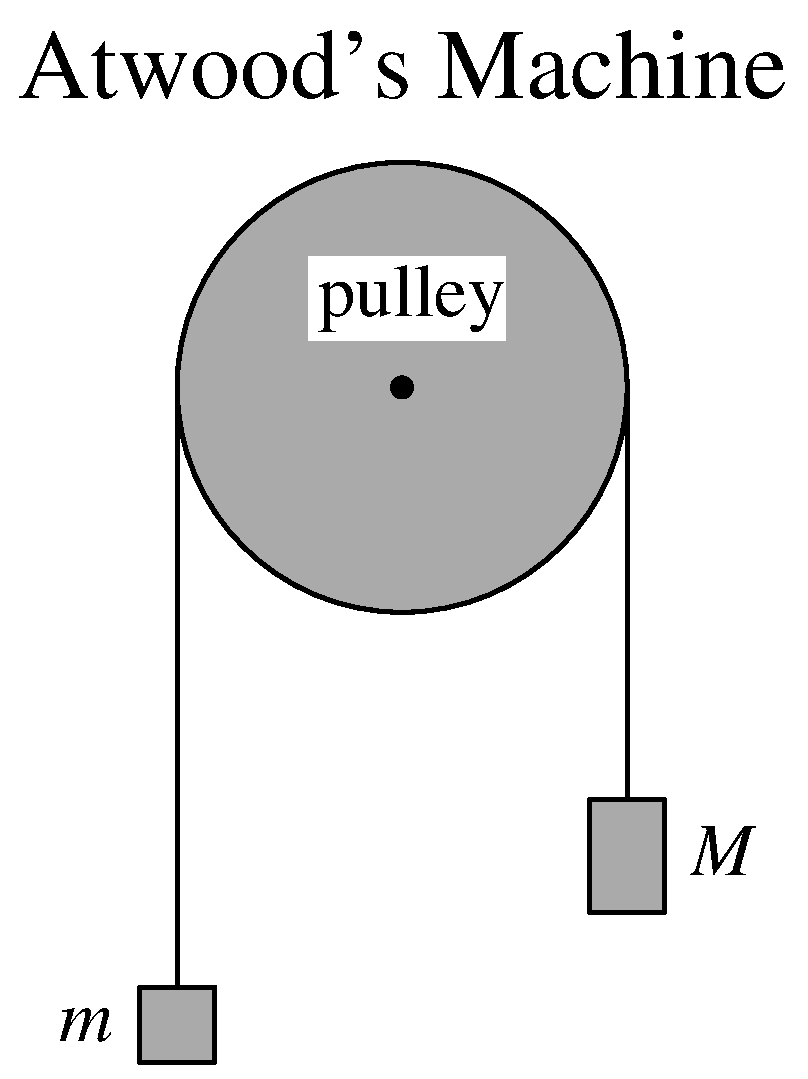
\includegraphics{atwood2.eps}}}}
\end{center}
%\vspace{3in}
%\special{eps:atwood.eps}
\caption{Diagram of Atwood Machine.
          \label{fig:atwood}}
\end{figure}

An Atwood machine is a device that uses weights and pulleys to test
Newton's second law, and to find the acceleration of the system of
masses shown Fig.~\ref{fig:atwood}.  In this experiment, we will use
the computer to record the
velocity of the masses as a function of time.  From these data, we can
calculate the acceleration.

Increasingly, scientists and engineers use computers to acquire data
automatically from experiments.  In this experiment, we will introduce
a hardware and software system designed by Pasco Scientific, which
allows us to 
%connect interface hardware through an SCSI port, and 
record data from a wide
range of apparatus automatically, using the Pasco ``Science
Workshop'' software for Windows.  We will use this same system in
other experiments in this course.



\section*{Apparatus and Procedure}

Please note first of all that the Pasco ``smart pulley" is fragile.
Be careful in working with it!  {\bf In particular, be sure that you
choose
a length of string such that it is impossible for the upward-moving
weight to strike the pulley!}

First notice how the pulley works.  There is a beam of light that
passes from one side of the pulley to the other.  As the pulley turns,
this light beam is interrupted by one of the pulley spokes, and a
signal is transmitted to the computer.  Thus, this system measures
directly the time from one interruption of the light beam to the next.
Since the pulley has ten spokes, we are measuring the time it takes
for the pulley to move through an angle of $36^\circ$ --- 1/10 of a
circle. If
we know the radius of the pulley, it is not hard to calculate how fast
the string on radius of the pulley is moving as the pulley turns.
We will be talking about how to do this calculation later in the
semester; but see if you can figure it out now.

{\bf NOTE:} The Pasco software uses a built-in ``calibration constant"
to convert these times into linear velocities.  Unfortunately, this
calibration constant is given to only two significant figures.  As a
result, there may well be a systematic uncertainty in the velocities
(remember our discussion from the Reaction Time experiment about the
difference between systematic and random uncertainties).

After your lab instructor shows you how the apparatus works, take some
time to become familiar with it.  See how the string fits over the
pulley, hang some masses from each end, and do a few test runs.  It
is probably best to keep accelerations reasonably small.  Here
are a few guidelines:
\begin{itemize}
\item Mount the pulley as high on the vertical rod as you easily can.
Be
sure the rod is stable, and does not tend to shake or vibrate easily.
%
\item Do not hang a total of more than about 600 grams from the pulley
(both sides).
%
\item Note that the larger the total mass, and the smaller the
difference
between the two masses, the smaller the acceleration should be.
%
\item {\bf Be absolutely sure, before you do any test runs, that your
string
is long enough that the upward-moving mass cannot strike the pulley! }
\end{itemize}

\section*{Taking the Data}

Here are some guidelines for taking a set of velocity vs.\ time data,
from which you can calculate the acceleration.
Use these guidelines to develop your own procedure, {\bf and describe
that
procedure in comprehensive detail in your lab book, WHILE YOU ARE IN
THE LAB TAKING THE DATA.}

We will take data for two separate sets of masses.  Try to choose
values for which the accelerations differ by at least a factor of two;
but keep both accelerations reasonably small.

For each set of masses, take four separate sets of data.  Thus, you
will have a total of 8 runs for this experiment.

Guidelines for taking data:
\begin{itemize}
\item Measure the masses carefully on the digital balance.  If you are
using more than one mass for either $m$ or $M$, measure the masses
together---do not measure the individual masses and add them later.
Why?
%
\item Set up the two masses on the string.  The lower mass should be
as close to the floor as possible.
%
\item Develop a procedure for releasing the masses---be sure they do
not have a tendency to sway as they move.
%
\item One should person click the RECord button on the Pasco screen, then the
other person releases the masses.
As soon as the descending mass
strikes the floor, click on the stop button.  You should now have a
set of data for velocity vs.\ time.   Examine the data on the graph in
the Pasco Science Workshop program, and be sure you understand how to
use it to find the acceleration of the masses.
%
\end{itemize}

\section*{Data Reduction and Analysis}
\subsection*{Using Linfit to find the acceleration}

We will move the data to Linfit to find the acceleration, using the
data for velocity vs.\ time that you have already recorded.  To do so:
\begin{itemize}
\item Start up Linfit.
%
\item Go back to the Pasco program, and select only those velocity vs.
time data that you want to fit.  Note that as you select the data on
the graph, it is also selected in the table. Select (click on) the table window.
%
\item Select ``Copy" from the Edit menu.
%
\item Now switch to Linfit, and pull up the spreadsheet.  Put the
cursor in the top left cell, and Paste your data into Linfit.
%
\item You will be taking eight sets of data.  
It is a good idea to save this file to disk frequently.
%
\item Select your data on the spreadsheet, move it to the data screen,
and do your least-squares fit to find the acceleration.
\begin{itemize}
\item For the uncertainty in velocity, use 0.003 m/sec.
(This estimate is based on limited experience; let your instructor
know if your reduced chi-squared value seems off.)
%
%\item Parameter estimates: Use your theoretical value of the
%acceleration for the slope; for the intercept, choose zero, since the
%initial speed of the masses will be small.
\end{itemize}
%
\item You do not need to print your fit; but do go back to the
spreadsheet, and from the Data menu, choose Data/Get Fit Results from
Fit Screen.  This step will open a new worksheet.  It might be easiest
to cut the slope and its uncertainty (the parameter $B$) and paste it
into the same worksheet with your data.
\end{itemize}

{\bf For each data set, you
should, at this point, have a value of acceleration, and the
uncertainty in the acceleration, from your least-squares fit.}

You
might also want to record your two masses on this worksheet, and
calculate the theoretical value of the acceleration.  Put enough text
in the worksheet so readers can easily see what each number
represents.  Include units, of course!


\subsection*{Uncertainty in the acceleration}
The uncertainty in each acceleration, which you obtain from your
least-squares fit, applies to that particular run.  But are there
variations from one run to the next?  We will investigate that
question in the following way:
\begin{itemize}
\item For each set of masses, collect the four values of the
acceleration that you found from your least-squares fits.
%
\item Calculate the average acceleration, the standard deviation, and
the standard deviation of the mean (see Appendix A, page~\pageref{sdev.mean}).
Note that the standard
deviation of the mean should represent the uncertainty in the
average acceleration.

As a check, see if the standard deviation of the mean is
consistent with the uncertainties from your least-squares fits.  (Note
that you can use a spreadsheet function to calculate the standard
deviation---see the on-line help.)
%� In addition, calculate the standard deviation of the mean.  What additional information does this quantity give you?
\end{itemize}

\subsection*{Analysis of the uncertainty in the theoretical value of
the acceleration}

As noted above, the theoretical value of the acceleration is given by

\[
 a = {{M - m} \over {M + m}}\; g
\]
We will want to compare this theoretical value with your experimental
values.  In order to do so, we must know the uncertainty in the
theoretical value based on the measured uncertainties in the masses
$M$ and $m$.  It turns out to be fairly difficult to calculate the
uncertainty in the acceleration $a$ using the techniques developed in
Appendix A of the lab manual,
so we will do it ``experimentally."  Change each mass (up and also down) by the measured
uncertainty (0.1 gm, for the digital balance that we use) and see what
happens to the acceleration.  Half the difference between the largest
and smallest calculated values of acceleration is a rough estimate of
the uncertainty.

\section*{Table of Results and Conclusion}

In most experiments, it is important to summarize all your
experimental results in your conclusions section.  For each set of
masses, make a table that includes
\begin{enumerate}
\renewcommand{\labelenumi}{(\alph{enumi})}
\item  the theoretical value of the acceleration, with uncertainty;
%
\item your value of the acceleration for each of your four runs with
that set of masses, with uncertainty (these values are the ones from
the least-squares fits); and
%
\item the average value and standard deviation of the mean for the
four measurements.
\end{enumerate}
If you want to, you can make this table up on a spreadsheet workbook,
and tape it into your lab notebook.
As always, put in enough text so that it can be read easily by someone else.
Make sure you display the proper number of significant digits
in these final reported results!

In your conclusion, you should discuss, separately for each set of
data, whether the theoretical and experimental values for the
acceleration agree, within the uncertainties of the experiment.  You
should also discuss whether the uncertainties in the least-squares
fits, in (b), are consistent with the standard deviations calculated
in (c).  If they are not, are there sources of systematic error that
might account for such an inconsistency?  (One is mentioned
above---the
calibration constant of the ``smart pulley;" what other systematic
errors might be present in this experiment?)



\renewcommand{\newname}{Kinetic Friction}
%KINETIC FRICTION
\newexp \label{exp:kinetic}
  

\section*{Before Lab} In this experiment, we will be investigate the
coefficient of kinetic friction.  In particular, we will measure
the acceleration of a system of masses, and use it to calculate the
coefficient of kinetic friction.

The first step is to derive an expression for $\mu_k$, the
coefficient
of kinetic friction.  You should do this derivation in your lab book
{\em before} you come to lab.  Your TA will check your notebook at
the beginning of the lab.

Here is a sketch of how to go about the derivation.  Consider the block
and pulley system shown in Fig.~\ref{fig:kinetic}.  Draw 
free-body
diagrams (one for each body), identifying all of the forces acting each mass.  Write
Newton's second law for each body.   Assume that the masses are
accelerating.

In class, we have often assumed $\mu_k$ was known and the acceleration
was unknown.
For this experiment, though, you will calculate the
coefficient of kinetic friction using the measured masses and
acceleration.  Consequently, you should solve these equations for the
coefficient of kinetic friction $\mu_k$.  Your
result should be
\setcounter{equation}{0}
\begin{equation}
	\mu_{k} = \frac{mg - (M+m)a}{Mg} \label{eq:kinfric}
\end{equation}
where $M$ and $m$ are the masses as shown in Fig.~\ref{fig:kinetic},
$a$ is the shared acceleration of the bodies, and $g$ is the acceleration
of gravity.

\section*{Introduction and Theory}
In class, we have assumed that the
coefficient of friction is constant---that is, it depends on only on the type of surfaces
in contact, and not on surface area, mass, or other parameters.  In
this lab we will measure the
coefficient of kinetic friction for the same two surfaces, but different
masses, velocities, accelerations, and surface areas, and see whether
or not the coefficient of friction is in fact constant.

Consider Eq.~\ref{eq:kinfric} above.  What does this equation tell us?
We know that the
coefficient of kinetic friction $\mu_{k}$ is assumed to be constant.
If it is, then the left side of Eq.~(\ref{eq:kinfric})
should always have the same value for any condition which results
in motion. 
Hence if we change the masses $M$ or $m$, the acceleration
$a$ should also change, so as to keep $\mu_k$
 the same.
% This makes sense because if a different mass is hung
%on the string it will change the motion of the sliding block.  Keep
%your equations handy in your notebook for later use.

In this experiment, we will use the Pasco computerized data
acquisition system to record the velocity of the falling mass $m$ in
Fig.~\ref{fig:kinetic} as a function of time, and use those data to
find the acceleration of the system.  Given the acceleration and the
masses, we can use Eq.~\ref{eq:kinfric} to find the coefficient of
friction $\mu_k$.

\section*{Apparatus}
Fig.~\ref{fig:kinetic} shows the experimental setup. You should have the following materials
available at your lab station:
\begin{enumerate}
\item Pasco interface box and Smart Pulley (the pulley with wire attached)
\item Table clamp
\item Mass and hanger set
\item Wooden blocks with hooks
\item String
\item Plastic horizontal surface on which the wood block slides
\end {enumerate}
\begin{figure}
\begin{center}
{\resizebox{4.5in}{!}{{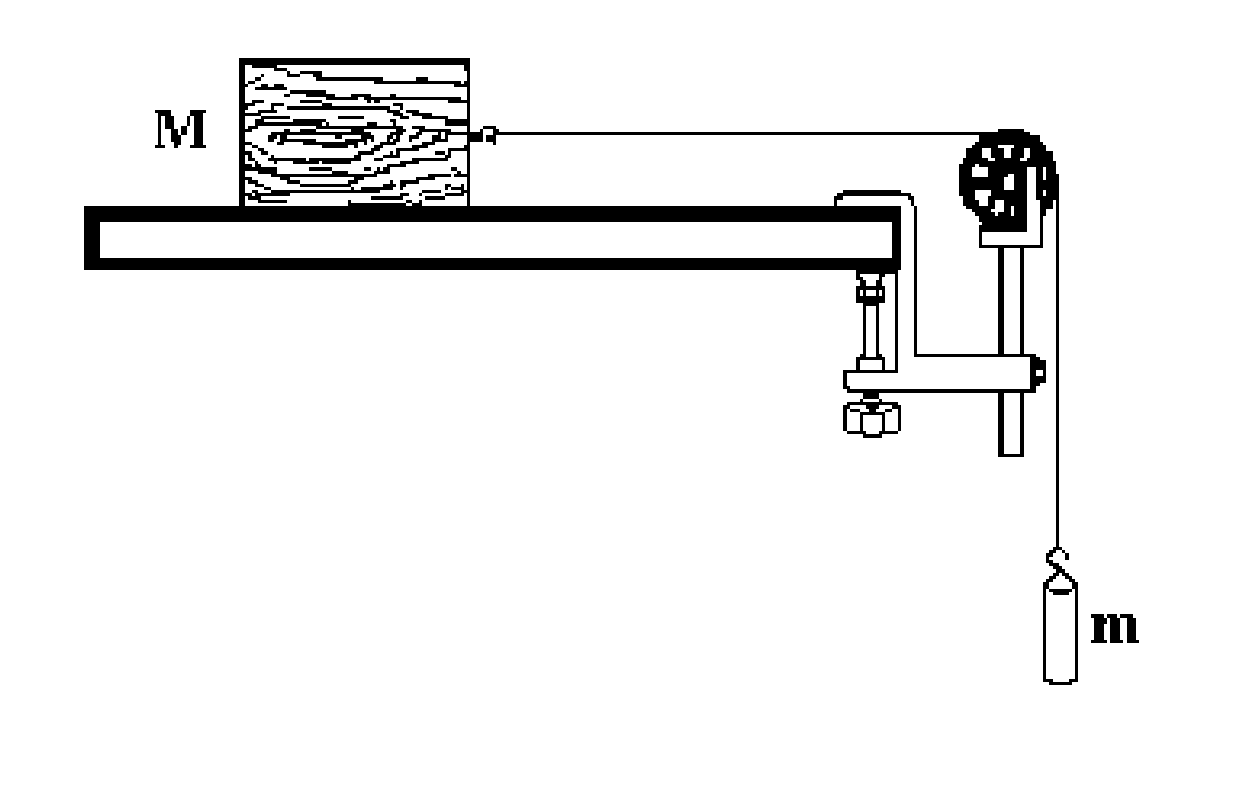
\includegraphics{kineticD.eps}}}}
\end{center}
% \vspace{3.5in}
%   \special{bmp:kinetic.bmp x=4.5in y=3in}
 \caption{Kinetic Friction Apparatus  \label{fig:kinetic}}
\end{figure}
The Smart Pulley should be connected to Digital Channel 1 on the Pasco interface box.
This device reads position by scanning the pulley spokes with a beam
of light.  It thus measures the angular velocity of the pulley.  The
computer uses the radius to convert angular velocity to the linear
velocity of the edge of the pulley---that velocity is of course equal
to the velocity of the descending mass.  All of this is exactly as in
the previous experiment.

\section*{Procedure}
Set up the apparatus as shown in the Figure.  Launch the DataStudio program,
Excel, and a web browser.
%, plug in your Smart
%Pulley, and turn on the computer if it isn't already on.  At this
%point you're ready to run the DataStudio program.  
Your TA
will give you specific instructions on the use of this software.

You will be taking a number of sets of data.  For each set, use the
procedure outlined below:

\begin{enumerate}
%
\item Place enough mass on the hanger so that the block will slide
on the table without needing an initial push (since we are measuring
{\em kinetic} friction).
%
\item Pull the block back until the mass $m$ is raised to the pulley.
Hold the block at rest until the next step.   {\bf Be sure that the string
is level.}
%
\item  When you are ready to take data, click Start in DataStudio and then release the block.
%
\item Now you can view the velocity vs.\ time data on a
DataStudio graph.  Copy and paste the linear portion of these data
to \WAPP and into a spreadsheet (as a backup copy; never print out
this data). Note that data pasted from DataStudio will include
text column labels which need to be deleted from the \WAPP ``Block Copy \& Paste"
web-form. Do a least-squares fit to find
the slope (that is, the acceleration).  You don't need to print the
fit report, but do record the acceleration (and its error) in your spreadsheet and notebook.
Note if the reduced chi-square signals a non-constant acceleration.
(Recall from previous experiment: $\delta v = .003\; {\rm m/s}$ and negligible error in time.)
%
\item For each mass $m$, do \underline{four} separate runs, and find the
acceleration for each.  

Find the average acceleration (spreadsheet function: {\tt average()}) and determine
its error using the standard deviation of the mean (spreadsheet function: {\tt stdev()/sqrt(4)}). Compare the
\WAPP reported errors in $a$ to the error in $a$ determined from
the standard deviation.  Are these error estimates
in the same ballpark (say within a factor of 2)? We will
use these results to find a value for $\mu_k$ (and its error)
for each mass $m$.  
%It may be convenient to save
%your data in a single spreadsheet file, with a separate worksheet page
%for each $m$.
%
\end{enumerate}
Follow the above procedure \underline{three} times
(for a total of 12 runs), each
time for a {\em different} mass $m$, keeping everything else constant.
%For each $m$, take data from four runs.  
Choose your values of $m$ to get
as wide a range of accelerations as possible---that way, we will be
measuring $\mu_k$ under a wide range of experimental conditions.
%

\section*{Data Reduction and Analysis}

For each $m$ calculate a value for $\mu_{k}$ using Eq.~\ref{eq:kinfric} and the average $a$.
Find the error in this $\mu_{k}$ using the ``high-low game" (see page \pageref{par:high.low.game}). 
(Note the maximum value of $\mu_{k}$ is achieved with:
$M^-$, $a^-$, and $m^+$.)
We use this method because a calculation of the uncertainty in
$\mu_{k}$ using the methods of Appendix A is fairly involved.  
This  crude method has
the advantage of simplicity but it
neglects canceling errors.

Make a final results table including $m$, $a$, $\mu_{k}$, and
the uncertainty in $\mu_{k}$.  
Somewhere in the table note the mass of the sliding block ($M$).

You will probably find that the velocity vs.\ time plots are not exactly
linear.  Often there will be a kink where the slope (acceleration)
changes appreciably.  Select such a data set and print out a copy of 
the graph (with fit line).  What do you think caused this behavior?

\subsubsection*{Spreadsheet Calculation}
In this lab you will be repeatedly calculating $\mu_k$ and $\delta \mu_k = (\mu_{k\; \rm high} -\mu_{k\; \rm low})/2$.
You may want to speed these calculations by  entering them as formulas in a spreadsheet.

\begin{center}
\begin{tabular}{|c|c|c|c|c|c|c|c|}
\hline
$M$ & $m$ & $a$              & $\delta a$      & $\mu_{k}$ & $\mu_{k}$ & $\mu_{k}$ & $\delta \mu_{k}$ \\
 (g)& (g) &  ${\rm (m/s^2)}$ & ${\rm (m/s^2)}$ &           & high      &  low      &  \\
\hline
 \phantom{10000}& \phantom{10000}   &  \phantom{10000}& \phantom{10000} & \phantom{10000} &  \phantom{10000}& \phantom{10000} &  \phantom{10000} \\
\hline
  &   &  &  &  &  &  &      \\ \hline
  &   &  &  &  &  &  &      \\ \hline
\end{tabular}
\end{center}

The formulas will depend on which columns contain which values; find below
an example.  (Since your columns may differ from those used in this example,
you need to understand this example, not just copy it!)
\begin{eqnarray}
\mu_k &= & {\tt (B2*9.8-(A2+B2)*C2)/(A2*9.8)}\\
\mu_{k\; \rm high}&=& {\tt ((B2+0.1)*9.8-(A2+B2)*(C2-D2))/((A2-0.1)*9.8)}\\
\mu_{k\; \rm low}&=& {\tt ((B2-0.1)*9.8-(A2+B2)*(C2+D2))/((A2+0.1)*9.8)}
\end{eqnarray}
While entering these formulas may look complex, once completed all further calculations
consist of just entering the data and ``pulling down the cell".

\section*{More experiments}

Do as many of the following additional experiments as time permits.  To save
time do not do the four repetitions to find $\delta a$, instead 
use the \WAPP reported error in $a$ to find $\delta \mu_{k}$.
\begin{enumerate}
\setcounter{enumi}{1}
\item Make another table of $M$, $\mu_{k}$, and $a$ (mass $M$ changing this time).
Do three runs, varying the mass $M$ of
the block each time, but holding the hanging mass $m$ constant.
You can change $M$ by setting masses on the block, but be sure you
start with enough mass $m$ on the hanger that it will always slide.
%In calculating the error in $\mu_{k}$,
%use the \WAPP reported error in $a$ rather than the standard deviation
%of the mean (since you will be doing just one trial for every
%$M$ value).
%
\item  Use masses from your first data set and compare what happens
if you slide the block {\em on its side}.  (Remember to adjust the
pulley height so the string is level!) This experiment will test
whether surface area affects
the kinetic friction coefficient.  Note results in your lab book, comparing the two sets
of data.
%
\item Try to get an estimate of the \underline{static} coefficient of friction
$\mu_{s}$ using the materials provided.
Is it higher or lower than $\mu_{k}$?  Record your results with error.
{\em (Note: you won't need the computer for this part---it's a
simple, but rough, estimate)}
%
%\item Calculate the error in $\mu_{k}$ using the values given by your TA for error in $a$, $m$
%and $M$.  Then compare this to the standard deviation of the mean of your values for $\mu_{k}$
%\item Summarize your results, answer the questions below, and turn in your notebook.
\end{enumerate}

\section*{Conclusions}
Consider your data, including uncertainties, and discuss the
following questions carefully and in detail:

A constant slope for a run implies a constant frictional
force during that run.  Did the frictional force seem to be constant during the runs?

Did the coefficient of friction vary
with acceleration? With surface area? With the mass of the block?

Overall, how good is our assumption that the coefficient of kinetic
friction is constant, within the limits of experimental error?


\section*{Critique of Lab}
     Follow the suggestions given in the Introduction to the
Laboratory Manual.

\section*{Quick Report Card}
Properly report (sigfigs, units, error) your three $\mu_k$ from the first part of the lab.
Record the masses used for the runs in which $\mu_k$ was measured.

%\newpage
%\cleardoublepage
%\begin{center}
% CHECKLIST - Kinetic Friction \\
%\end{center}
%\bigskip
%\begin{center}
%\begin{tabular}{||l|r||}
%ASPECT CONSIDERED & DONE? \\ \hline
%Prelab experiment and proof & \\ \hline
%Table of $m$, $a$, $R$, and $\mu_{k}$ with units and uncertainties & \\ \hline
%Table of $M$, $a$, $R$, and $\mu_{k}$ with units and uncertainties & \\ \hline
%Evaluation of surface area data & \\ \hline
%Summary of results & \\ \hline
%Calculated uncertainties $\delta \mu_{k}$, Compare to $\sigma_{\bar x}$ & \\ %\hline
%Questions answered & \\ \hline
%Cleanup & \\ \hline
%\end{tabular}
%\end{center}
\bigskip
\bigskip
\bigskip

%%COMMENTS:\\
%\newpage
%\newpage
%\bigskip
%\begin{center}
%{\bf Pre-Lab}
%\end{center}
%\centerbmp {4in}{2in}{coin.bmp}
%Perform the following
%mini-experiment: Get a book, a coin, and a ruler.  Place a coin on your closed book.
%Now tilt the book until the coin begins to slide, then lower it until it slides
%down the book at a constant speed. Note this position, then measure
% the angle $\theta$ the book is tilted (by measuring
%two sides of the ``triangle'').  Now calculate the friction coefficient,using
%$\tan \theta = \mu$ and record
% your results.  Question: Is the $\mu$ you just found the Kinetic or Static friction coefficient?  Derive the equation $\tan \theta = \mu$ starting with Newton's Second Law.
%
% {\em Hint: Sum the forces on the coin in the x direction (parallel to the table top), finding the components of N and the frictional
%force.  Then substitute the definition of the frictional force and solve for
%$\mu$.}
%\bigskip

\renewcommand{\newname}{Ballistic Pendulum}
%BALLISTIC PENDULUM
\newexp

\section*{Before Lab}

Please read this writeup carefully, and be sure you can derive
Equations (\ref{v(y)}) and (\ref{y(xL)}).  Work out these
derivations in your lab notebook.  Your TA will check them at the
beginning of the lab period.  It may also be helpful to review the
concepts of standard deviation and standard deviation of the mean.

\section*{Introduction}

In a collision the total momentum of the colliding bodies is
unchanged---that is, momentum is conserved---if the net external force is
zero.  However,
mechanical energy may or may not be conserved.  In the study of
collisions, two extremes are generally
defined.  A {\em perfectly elastic} collision is one in which the
total kinetic energy of the system doesn't change.  Collisions of
microscopic objects such as atoms, for example, often fit into this
category.  If the kinetic energy is changed following the collision, 
the collision is inelastic.  A {\em perfectly
inelastic} collision is one in which the colliding objects stick
together.  In this experiment we will use a device known as a
ballistic pendulum to study inelastic collisions and to measure the
velocity of a projectile.

%You will also get practice with some basic
%statistical analysis techniques.

\section*{Apparatus}
\be
\item Projectile launcher, steel ball;
\item Ball catcher suspended from an aluminum rod;
\item Steel rail with tinfoil marker;
\item Tape measure and scale (somewhere in the lab);
\item Plumb line;
\item Meter stick.
\ee
\section*{Experiment}

In this experiment we will be shooting a steel ball horizontally from
a launcher, as illustrated in Fig.~\ref{bpend}.  The ball will be
caught by a cylindrical container suspended as a pendulum from strings
mounted on an aluminum rod.  By measuring the horizontal distance the
pendulum swings we can calculate the ball's initial velocity $v$.

We will compare this result with the velocity calculated by shooting
the projectile horizontally and measuring how far it travels.

%With this information you should also be able
%to determine how far the launcher can shoot the ball.

%\newpage
%\vspace*{2in}
\bfig
\begin{center}
{\resizebox{5.5in}{!}{{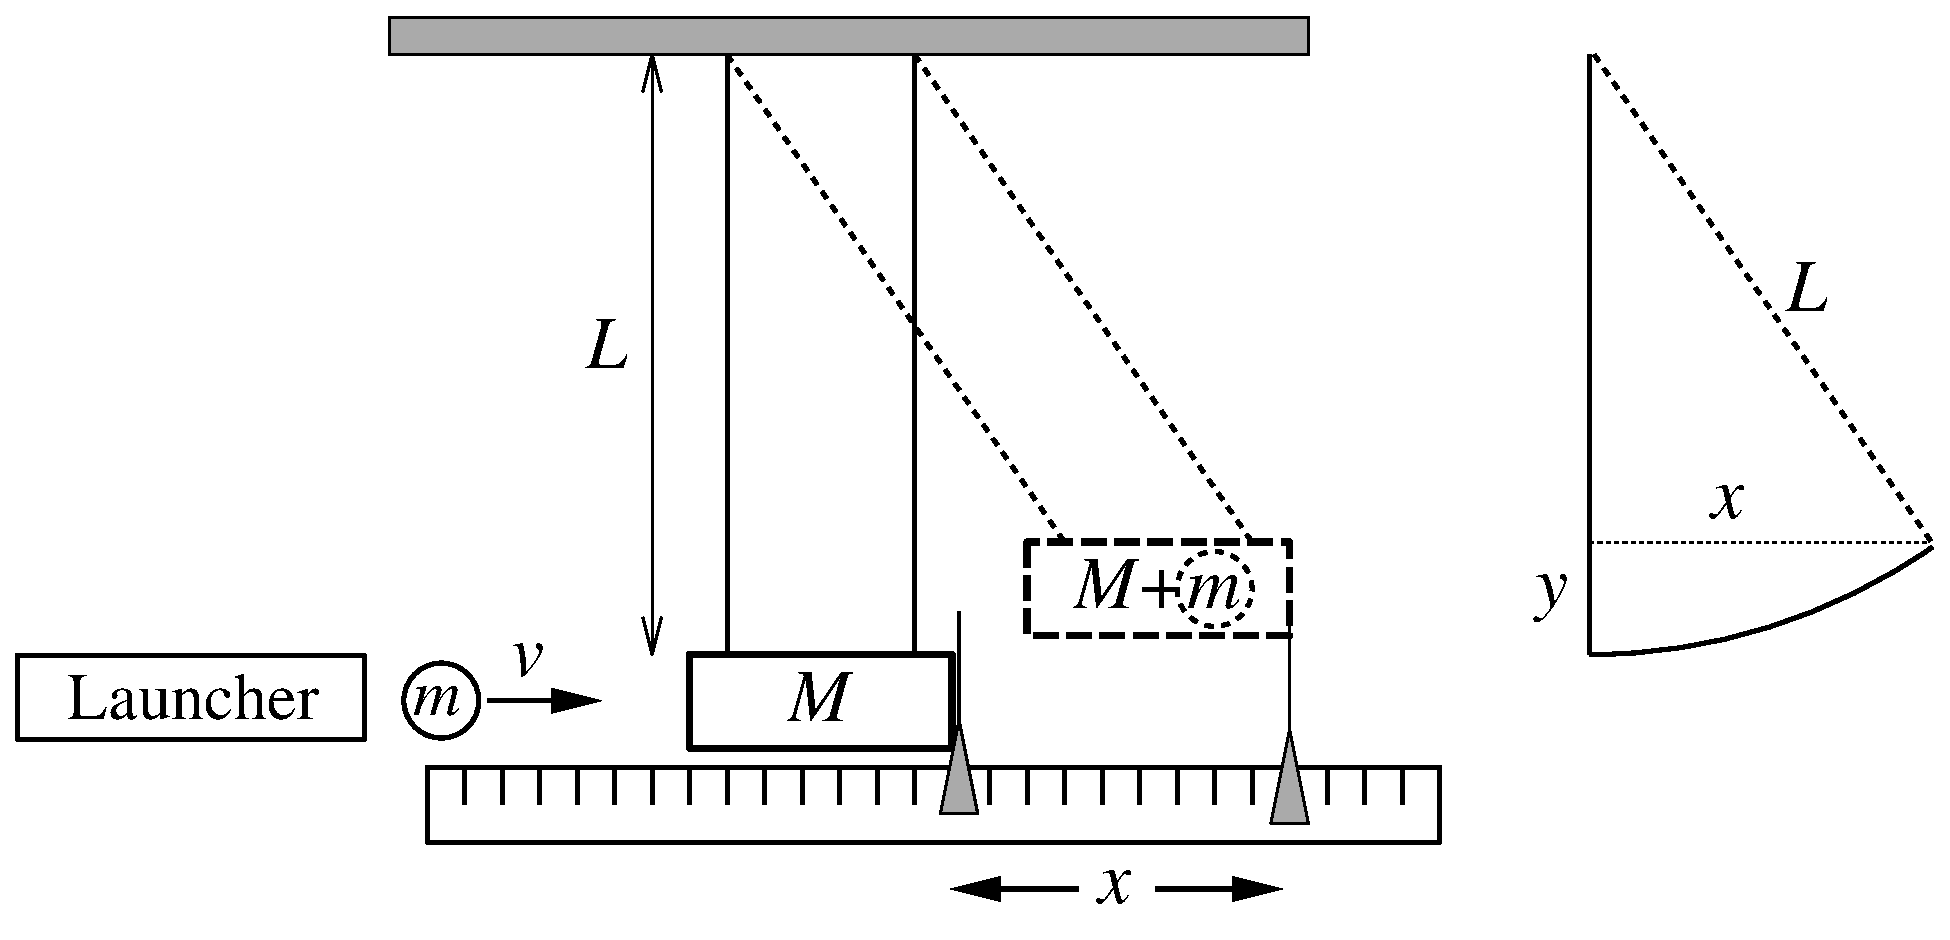
\includegraphics{ballis2.eps}}}}
\end{center}
%\special{eps:\location ballis1.eps x=5.5in y=2in}
%\special{eps:ballis1.eps x=5.5in y=2in}
\caption{Ballistic pendulum experiment. \label{bpend}}
\efig

\section*{Theory}

Consider Fig.~\ref{bpend} above:  We launch a
%spherical steel projectile
steel ball 
at a cylindrical ``catcher.''  The two collide and stick together, and
thereafter move as one.  It is convenient to divide this process
conceptually into two parts.

First part: During the collision itself, momentum is conserved, but
energy is not, since the collision is perfectly inelastic.  Thus, the momentum
$p_{i}$ before the collision equals $p_{f}$, the momentum after the
collision.  In equation form,

\beq
p_{i} = mv = p_{f} = (m+M)V, \label{pi=pf}
\eeq

where $m$ is the ball's mass, $M$ is the catcher mass, $v$ is the
ball's initial velocity and $V$ is the velocity of the catcher and
ball immediately after the collision.

Second part:  Immediately after the collision, the ball/catcher system
becomes the bob of a pendulum that moves off at some initial velocity
$V$, given in Eq.(\ref{pi=pf}) above. The pendulum's initial
kinetic energy changes to gravitational
potential energy as it swings and rises to a height $y$, where it is
instantaneously at rest. Momentum is clearly not
conserved in this second part of the experiment as the
pendulum slows, stops, and reverses. The motion
of the system is nearly frictionless, so mechanical energy {\it is} nearly
conserved for this part of the motion.  We express this conservation
law in the equation

\beq
\frac{1}{2}(m+M)V^{2} = (m+M)gy. \label{KE=PE}
\eeq

If we combine Eqs.~(\ref{pi=pf})~and~(\ref{KE=PE}), it is easy to
show that the initial velocity of the projectile is related to the
height $y$:

\beq
v = \left(1+\frac{M}{m}\right)\sqrt{2gy}. \label{v(y)}
\eeq

It would be difficult to measure the change in height $y$ directly.
Instead, we will measure the horizontal distance $x$ that the pendulum
moves, and use this quantity to calculate $y$.  If we consider
Fig.~\ref{bpend}, it is clear the the string length $L$ is
the hypotenuse of a right triangle with sides $(L-y)$ and $x$, so:

%\beq
%L^{2} = x^{2} + (L-y)^{2} = L^{2} + x^{2} + y^{2} - 2Ly, \label{quad}
%\eeq
%which is a quadratic equation for $y$ with the solutions
%\beq
%y = L \pm \sqrt{L^{2}-x^{2}}. \label{y(xL)}
%\eeq
%The minus sign gives the solution which is relevant here.  (Can you
%explain what the other one means?) So by measuring $x$, the initial
%velocity $v$ of the ball can be calculated.

\beq
L^2 = (L-y)^2 + x^2
\eeq

If we subtract $x^2$ from both sides we obtain

\beq
L^2 - x^2 = (L-y)^2.
\eeq

If we now take the (positive) square root and solve for $y$,
we find

\beq
y = L - \sqrt{L^{2}-x^{2}}. \label{y(xL)}
\eeq

We will use this expression for $y$ in Eq.~(\ref{v(y)}) above to
calculate $v$.

We also want to find the uncertainty in the initial projectile
velocity $v$.  The measured quantities, $x$, $L$, $m$, and $M$ all
have some uncertainty, leading to uncertainty in the calculated $v$.
The formulas connecting $v$ with these measured quantities would make
the error analysis complicated.  In addition, another source of
uncertainty is in the behavior of the launcher---one sometimes sees
variations in $v$ from shot to shot.

Under these circumstances, a good way to estimate 
uncertainty is repeated measurement.
%both the velocity
%and the uncertainty in the velocity is to fire the ball repeatedly,
%and calculate the mean velocity and the standard deviation of the mean
%as an estimate for the uncertainty.  
Suggestions for a detailed
procedure are given below.

%Finally, we can calculate the change in kinetic energy.  Kinetic
%energy will be lost in any non-elastic collision. In the {\em
%perfectly} inelastic case, one can readily show from Eq.~(\ref{pi=pf})
%that
%
%\beq
%\frac{KE_{{\rm before}}}{KE_{{\rm after}}} =
%\frac{\frac{1}{2}mv^{2}}{\frac{1}{2}(m+M)V^{2}} = \frac{m+M}{m}
%\label{KEratio}
%\eeq



\section*{Procedure and Data Analysis}

\be

%\item BEFORE YOU COME TO LAB: Do the algebra to obtain
%Eqs.~(\ref{v(y)}), (\ref{y(xL)}), and (\ref{KEratio}).  Be ready to
%show all this to your TA, or to deal with these concepts on a quiz.

%\item

\item Use the digital balance to measure the masses $m$ and $M$ of the
ball and catcher.  (The mass of the catcher may already be given.) 
Use the tape measure to measure the string length
$L$, {\it after} you have completed the alignment procedure described
below. Record these values (with uncertainties) in your notebook.

\item  Alignment Procedure for the Ballistic Pendulum

Identify the projectile launcher, the catcher, and the foil slider.
Be sure that the launcher on your table is mounted so that it shoots
horizontally.  Be sure that it positioned close to the catcher.

It is {\bf important} that the projectile launcher, catcher, and foil
slider all be aligned along the same axis.  Each must also be
level.  Take your time, and be sure follow this procedure carefully.

	\begin{itemize}

	\item  To align along the same axis, place the slider track
	under the catcher and clamp the launcher in place.  Looking
         down the slider track, all three should appear to line up.
	
	\item The height of the catcher can be adjusted by raising or
	lowering the vertical rod holding the catcher in place. 
       The string support 
        can be leveled by loosening the support clamp and rotating the
        topmost support assembly.  The
	catcher should barely clear ($\sim 1/8"$) the slider
	track.  The catcher should also be at the same level as the
	launcher.
	
	\item The launcher can be leveled by loosening a wing nut
and rotating it.
	The catcher can be leveled
        by pulling string through the catcher.  
	
	\end{itemize}


\item Loading the Launcher

	\begin{itemize}

	\item The ball should be inserted into the launcher with the
        wooden dowel.  Notice that there are three settings for the launch
        velocity --- denoted by ``clicks."  Always listen for the same number of clicks.
        (We have had the best luck using full force: three clicks.)

	\item  Use the same wooden dowel to remove the ball from the
        catcher.  To accomplish this, pull the catcher to one side of
        the track and push the dowel into the far end of the catcher.
	
	\item Take some practice shots to make sure everything works
        correctly.  Make sure the tinfoil marker slides with hardly
        any resistance on the rail.  Make sure the catcher swings
        upward without rotating.  If there are problems check with
        your TA.
	
	\end{itemize}


\item Positioning the Foil Slider

	\begin{itemize}

	\item Take an initial measurement by pushing the slider
         against the catcher and firing.  The new position of the
         slider will determine the horizontal distance moved.

	\item  For subsequent measurements, start with the slider
        placed about 1 cm short of the expected final position.
        Occasionally check the apparatus to make sure nothing has
        moved out of position.
	
	\end{itemize}

\item After taking several practice shots,
start recording the distances $x$ that pendulum moves.
Repeat this process, so that you have  five good 
measurements of $x$.  

%Use spreadsheet functions
%{\tt AVERAGE(...)} and {\tt STDEV(...)}
%to calculate
%the average $\langle{x}\rangle$ and standard deviation $\sigma_{x}$.  
%Use the standard deviation of the mean as the error in $x$.

\item Find  the {\tt average(...)} and  {\tt stdev(...)} of these five
measurements of $x$; use these values for $x$ and $\delta x$ in the following
calculation.

% to calculate four values for
\item Calculate the best estimate for the speed $v$, by combining Equations (\ref{y(xL)}) and (\ref{v(y)}).
The usual methods of error propagation are rather difficult to apply to this
complex equation, so we again fall back to the ``high-low" method of error analysis.
The high value for $v$ is obtained from: $M^+$, $m^-$, $L^-$, $x^+$.
This calculation can be made tolerable by using   a spreadsheet  to repeatedly
apply the complex formula for the slightly changed values of
$M$, $m$, $L$, and $x$.  Put these values
in a row of adjacent  cells in a spreadsheet
and write (in the following cell) the formula for $v$, using 
cell-values for $M$, $m$, $L$, and $x$.
If you now copy and paste these five cells directly below
the original set, you have the ability to modify each of the measured
quantities and see how that affects $v$.  %You can now play the ``high-low game"
%to determine the error in $v$.  Note that the high estimate for
%$v$ is obtained from $M^+$, $m^-$, $L^-$, $x^+$.

%Then
%use spreadsheet functions {\tt AVERAGE(...)} and {\tt STDEV(...)}
%to calculate the average velocity and standard deviation.  Use the standard
%deviation of the mean as the uncertainty in $v$.

%Note that this method does not take into account uncertainties in the
%masses and the length of the string---be sure you understand why.  So
%make these measurements as accurately as you can.  We are thus, in this
%experiment, treating these quantities as systematic uncertainties.

%\item The formula for $v$ is fairly complicated, involving the
%measured quantities

\item Now test this measurement  of $v$ by predicting the
range $D$ of the projectile in a purely horizontal
shot.
If we consider only the
vertical motion, it is easy to show that the ball will fall the
distance $h$ to the floor in a time

\beq
t = \sqrt{\frac{2h}{g}}
\eeq
During that time the ball will
travel a horizontal distance $D$ at an unchanging horizontal
velocity equal to the initial velocity.  The horizontal  distance will therefore be

\beq
D = vt 
\eeq
Calculate $D$ and see if experiment matches your prediction!
Position
the launcher at the edge of the table, and  measure $h$.  Use the
plumb line and a piece of masking tape to mark the initial position of
the ball on the floor.  Place paper and carbon paper to mark
where the projectile actually hits. Be sure the launcher is horizontal and 
and aimed (left/right) accurately!
Notify your TA when you are ready to test
your prediction.  Prizes will be awarded to groups able to hit the mark
on the first try!

\item Reversing this process, you can make
several measurements of the horizontal distance $D$ that the ball
travels and calculate $v$:
\beq
v = {D\over \sqrt{\frac{2h}{g}}} = D \sqrt{\frac{g}{2h}} =\sqrt{\frac{g}{2}}\;{D\over h^{1/2}}
\eeq
Use the spread in hit locations to estimate $\delta D$.
Use the Eq.~(E.11) to find the resulting error in the calculated value of
$v$.
%The velocity calculated in this way should agree, within
%experimental uncertainty, with that found in the first part of the
%experiment.

%and calculate the expected limits of $R$ using your $\overline{v} \pm
%\sigma_{\overline{v}}$ values.

%\item Measure and mark on the floor the region where you expect the
%ball to land.  (A plumb line may be helpful for determining where to
%measure from on the floor.) Notify your TA when you are ready to test
%your prediction.

%\item In your lab report, calculate the amount of kinetic energy initially
%before the collision and final potential energy when the pendulum
%reaches its full swing.  What do you think
%became of the difference?  When was most of this energy ``lost"?

%\item Make any other comments on collisions, ballistic pendulums, this
%equipment, etc.  Get your lab report finished, include the Evaluation
%page as usual, and turn it in.

\ee

\section*{Conclusions}
Report both values for the ball's initial
velocity (each with an uncertainty).
Do your two values agree within experimental
uncertainty?  If they do not, what might account for the discrepancy.
Were you able to predict where the projectile would land? (By how much
did you miss?)
Give a careful, detailed discussion of
your results.  How well did the experiment work?  What problems did you encounter?
How might the experiment be improved?

%Also report your results for the kinetic energy of the system before
%and after the collision.  What happened to the ``missing'' kinetic
%energy?

\section*{Critique of Lab}

Follow the suggestions given in the introduction to the Laboratory
Manual.

\section*{Quick Report Card}
Properly report (sigfigs, units, error) your two values for $v$
and if you hit the mark on your first try.


%\newpage
%\cleardoublepage
%\bc
%\bt{||l|r||}
%ASPECT CONSIDERED & EVALUATION \\ \hl
%Quiz              &            \\ \hl
%Lab report turned in on time & \\ \hl
%Measurements of $m$, $M$, $L$ & \\ \hl
%Spreadsheet analysis of $x$ data & \\ \hl
%Comments on consistency of launcher & \\ \hl
%Spreadsheet calculations of $v$,$\overline{v}$,$\sigma_{\overline{x}}$ & \\ \hl
%Range calculation and success of prediction & \\ \hl
%Comparison of KE before and after collision, and comments & \\ \hl
%Overall completeness of lab report & \\ \hl
%\et
%\ec
%GRADE (0-10) \underline{\hspace*{10em}} \\
%\bigskip
%COMMENTS:
%\vfill
%\ \dotfill \ \\
%EXPERIMENT \thechapter: \newname\\
%\bigskip
%Student \underline{\hspace*{10em}} \hfill Grade:(0-10) \underline{\hspace*{5em}} \hfill TA: \underline{\hspace*{5em}} \hfill \\
%Comments:
%\vfill




\renewcommand{\newname}{Two-Body Collisions}
%TWO BODY COLLISIONS
\newexp
\section*{Introduction}
Outside of Chicago at Fermilab, protons going $.999999\times c$ slam
into iron nuclei: a little collision problem involving conservation of momentum
and conservation of energy.
%     High energy physics often involves conservation of momentum and
%conservation of energy principles.  When high energy particles from an
%accelerator bombard the particles in a target we have a collision
%problem.  
The purpose of this experiment is to study the fundamentals of
collisions by analyzing the momentum and energy aspects of a two body
collision.  When the collision involves only two particles, the
trajectories of the particles before and after the collision lie in a
plane.  Therefore analysis in two dimensions is all that is necessary
to exactly solve this problem.% involving a two body collision.
\begin{figure}
\begin{center}
{\resizebox{3in}{!}{{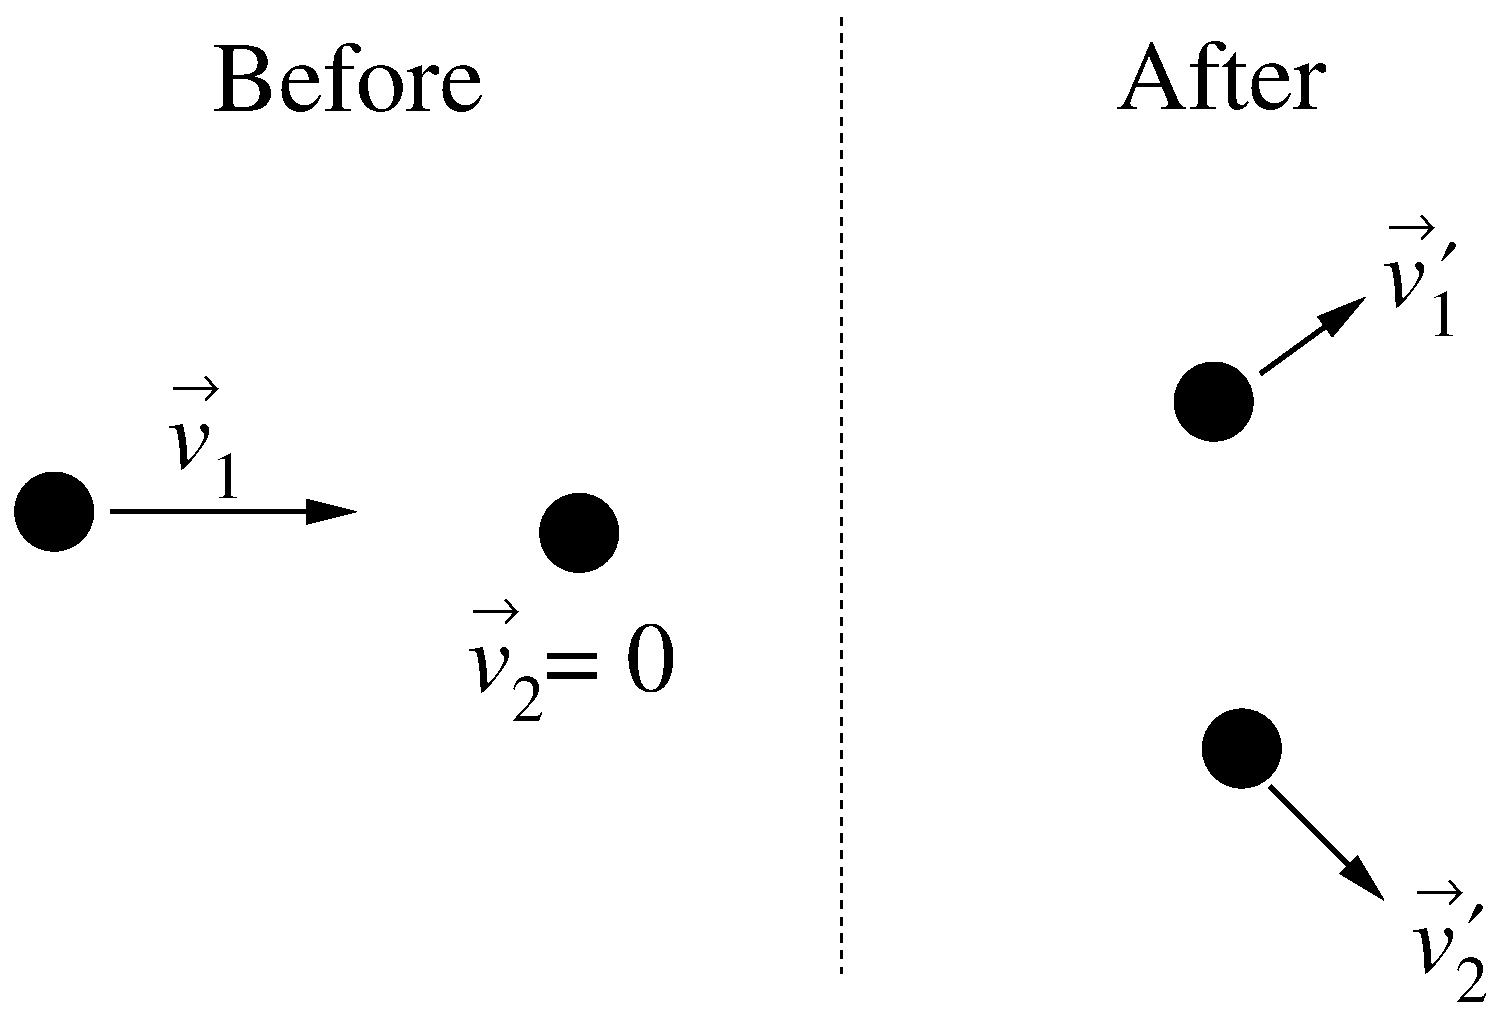
\includegraphics{2-body.defs.eps}}}}
\end{center}
%\vspace{2.5in}
%\special{ps:fig6_1.ps}
\caption{Diagram of a two body collision showing the situation before and
   after the collision.  \label{fig:tb1}}
\end{figure}

\section*{Analysis of Problem}
     In any collision, the total momentum of the colliding bodies is
unchanged by the collision.  Consider the case of a steel ball of mass
$m_{1}$ moving with velocity $\vec{\,v}_{1}$ colliding with mass $m_{2}$ initially at
rest.  (See Figure~\ref{fig:tb1}.)
After the collision the masses move off with velocities $\vec{\,v}_{1}'$ and $\vec{\,v}_{2}'$.
The law of conservation of momentum demands that the total momentum
before the collision, $\vec{P}$, is equal to the total momentum after the
collision, $\vec{P'}$.
\[
\vec{P} = \vec{P'}
\]
or
\begin{equation}
m_{1} \vec{\,v}_{1}  = m_1 \vec{\,v}_{1}' + m_2 \vec{\,v}_{2}'  \label{eq:tb1}
\end{equation}
     Remember that this vector equation actually represents
three equations, one for each coordinate direction.  In this experiment
we will observe collisions in two dimensions and only two of the three
equations will be used.  If the colliding objects are in the $x$-$y$ plane
we can write:
\begin{equation}
P_{x} = P_{x}' \qquad : \qquad m_1 v_{1x} = m_1 v_{1x}' + m_2 v_{2x}'
    \label{eq:tb2a}
\end{equation}
and
\begin{equation}
P_{y} = P_{y}' \qquad : \qquad m_1 v_{1y} = m_1 v_{1y}' + m_2 v_{2y}'
    \label{eq:tb2b}
\end{equation}
Here the $x$, $y$ subscripts denote the component of velocity along the $x$
 and $y$
axes.  It is convenient to set up the coordinate system so that $v_{1y} = 0$.
The Equations~\ref{eq:tb2a}~and~\ref{eq:tb2b} hold for any two dimensional
collision with one particle initially at rest.

     Kinetic energy is not necessarily conserved in a collision.  In the
case of two colliding steel balls about 10\% of the initial kinetic
energy is converted to heat and sound during the collision.  The total
kinetic energy before the collision in Figure~\ref{fig:tb1} is given by
\begin{equation}
E = {{1} \over {2}} \, m_1 v_{1}^{2}  \label{eq:tb3}
\end{equation}
 After the collision the total kinetic energy is
\begin{equation}
E' = {{1} \over {2}} \, m_1 \left( v_{1}' \right)^{2} + {{1} \over {2}} \,
      m_2 \left( v_{2}' \right)^{2}  \label{eq:tb4}
\end{equation}
 The percentage energy lost in the collision is
\begin{equation}
\mbox{\% loss} = {{E - E'} \over {E}} \times 100\%  \label{eq:tb5}
\end{equation}
     In this experiment we will use a curved aluminum ramp to accelerate
a steel ball and shoot it horizontally.  This ball strikes a second ball
at the end of the ramp.  Immediately after the collision both balls will
be traveling nearly horizontally; but they will simultaneously fall to the
floor because of the effect of gravity.  The time it takes to fall to
the floor is independent of the horizontal velocities or the masses of
the balls.  Therefore the horizontal displacement $d$ of either ball from
the point of collision is directly proportional to $v'$, the velocity of
that ball immediately after the collision.
\begin{equation}
v' = {d\over t}  \label{eq:tb6}
\end{equation}
where $t$ is the constant fall-time.% that 
%is independent of the mass or horizontal velocity of the ball.
Calculations are much simplified if we invent a unit of time
(a {\em shake}) exactly equal to $t$.  Then $d$ is directly the
velocity in units of cm per shake.

%      In this experiment we will deal with relative measurements and
% simply forget about the constant $C$ even though it has units.  We will
% measure a quantity proportional to the velocities $v'$ of the balls by
% measuring the horizontal distance they travel after the collision.  In a
% sense we are measuring velocity in centimeters (per fall-time).  This procedure may seem
% a bit unusual, but remember we are simply ignoring the constant $C$ in
% Equation~\ref{eq:tb6} which is the same for both balls and has the proper
% dimensions to make the units come out correctly.

\section*{Experimental Procedure}
     Make sure that the apparatus is securely clamped to the lab table.
({\bf NOTE:}  Be sure to use the large bench clamps --- ordinary C clamps don't
seem to hold the apparatus securely enough.)  Tape a large piece of
paper to the floor near the lab table.  Choose two
steel balls of equal diameter (the 1/2 inch balls work well) and weigh
each ball to make sure that their masses do not differ by more than a
few percent.  This way you need not worry about which ball is which
during the experiment.

%    As a released ball rolls down the ramp, gravitional potential
%    energy is converted into kinetic energy.  If the center of mass
%    of the ball falls some vertical distance $\Delta z$, you might conclude
%    that the horizontal speed at the bottom of the ramp was given by:
%    \[
%    mg \: \Delta z = 0.5 m v^{2}
%    \]
%    In fact some of the gravitional potential energy rotational kinetic
%    energy, so as a result the horizontal velocity is reduced and is given by:
%    \[
%    mg \: \Delta z = 0.7 m v^{2}
%    \]
    
Mark a spot on the ramp and  release a ball from that spot.
and let it roll down the
ramp and strike the floor.  Release the ball smoothly without spinning or
pushing it. 
%Do not release the ball from the top
%of the ramp\ldots this gives poor results.  The height should be less than
%8 vertical cm from the table top. 
Now that you know where the ball will hit the floor, place a piece of
carbon paper (carbon side down) at that spot and release the
ball down the ramp again.    Repeat the procedure five times.
Estimate by eye the average
position of the marks made by the ball and the range of deviation.  
Record this distance ($x$) and its deviation (both $\delta x$ and $\delta y$) as
the initial velocity $\vec{\,v}_1$ and its error.
Draw on the paper the line that represents the path of the ball;
this line defines your $x$ direction and the vector $\vec{\,v}_1$.
Do not move this sheet of paper or the launcher until you complete this lab!

{\bf FYI:}  As the ball rolls down the ramp it acquires both translational
       and rotational kinetic energy.  As a result the translational
velocity is less than that calculated ignoring rotation---that's why
in this lab we measure $\vec{\,v}_1$ rather than calculating it from
the ramp height $\Delta z$. The following equation (not used in this lab, but which you
       will learn to derive a bit later in the semester) takes into
       account both the translational kinetic energy of the center of
       mass, and the rotation of the spherical ball around an axis
       through the center of mass:
\[
mg \: \Delta z = 0.7 m v^{2}
\]
     Now we are ready to record the results of a two-body collision on
the same sheet of paper.  Place a target ball on the dimpled screw platform
at the bottom of the ramp.  Make sure its height matches that of the projectile
when the projectile is at the bottom of the ramp.
Release the other ball from the same position on
the ramp that you used with the single ball trials.
Observe where each ball strikes the paper.  As before, place a
piece of carbon paper at these positions to record further collisions.
%Lift the carbon paper and circle and number the pairs of marks after each
%collision run.  
Make five duplicate collision runs.
Estimate by eye the average
position of the marks made by the ball and the range of deviation.  
As in Fig.~\ref{fig:tb2}, draw in the $x$ and $y$ legs of both displacement
vectors.  Note  these two displacement vectors have different origins:
the projected location of each ball's center at the moment of collision.
Measure and record the legs and deviations.


\section*{Analysis of the Data}
\begin{figure}
\begin{center}
{\resizebox{5in}{!}{{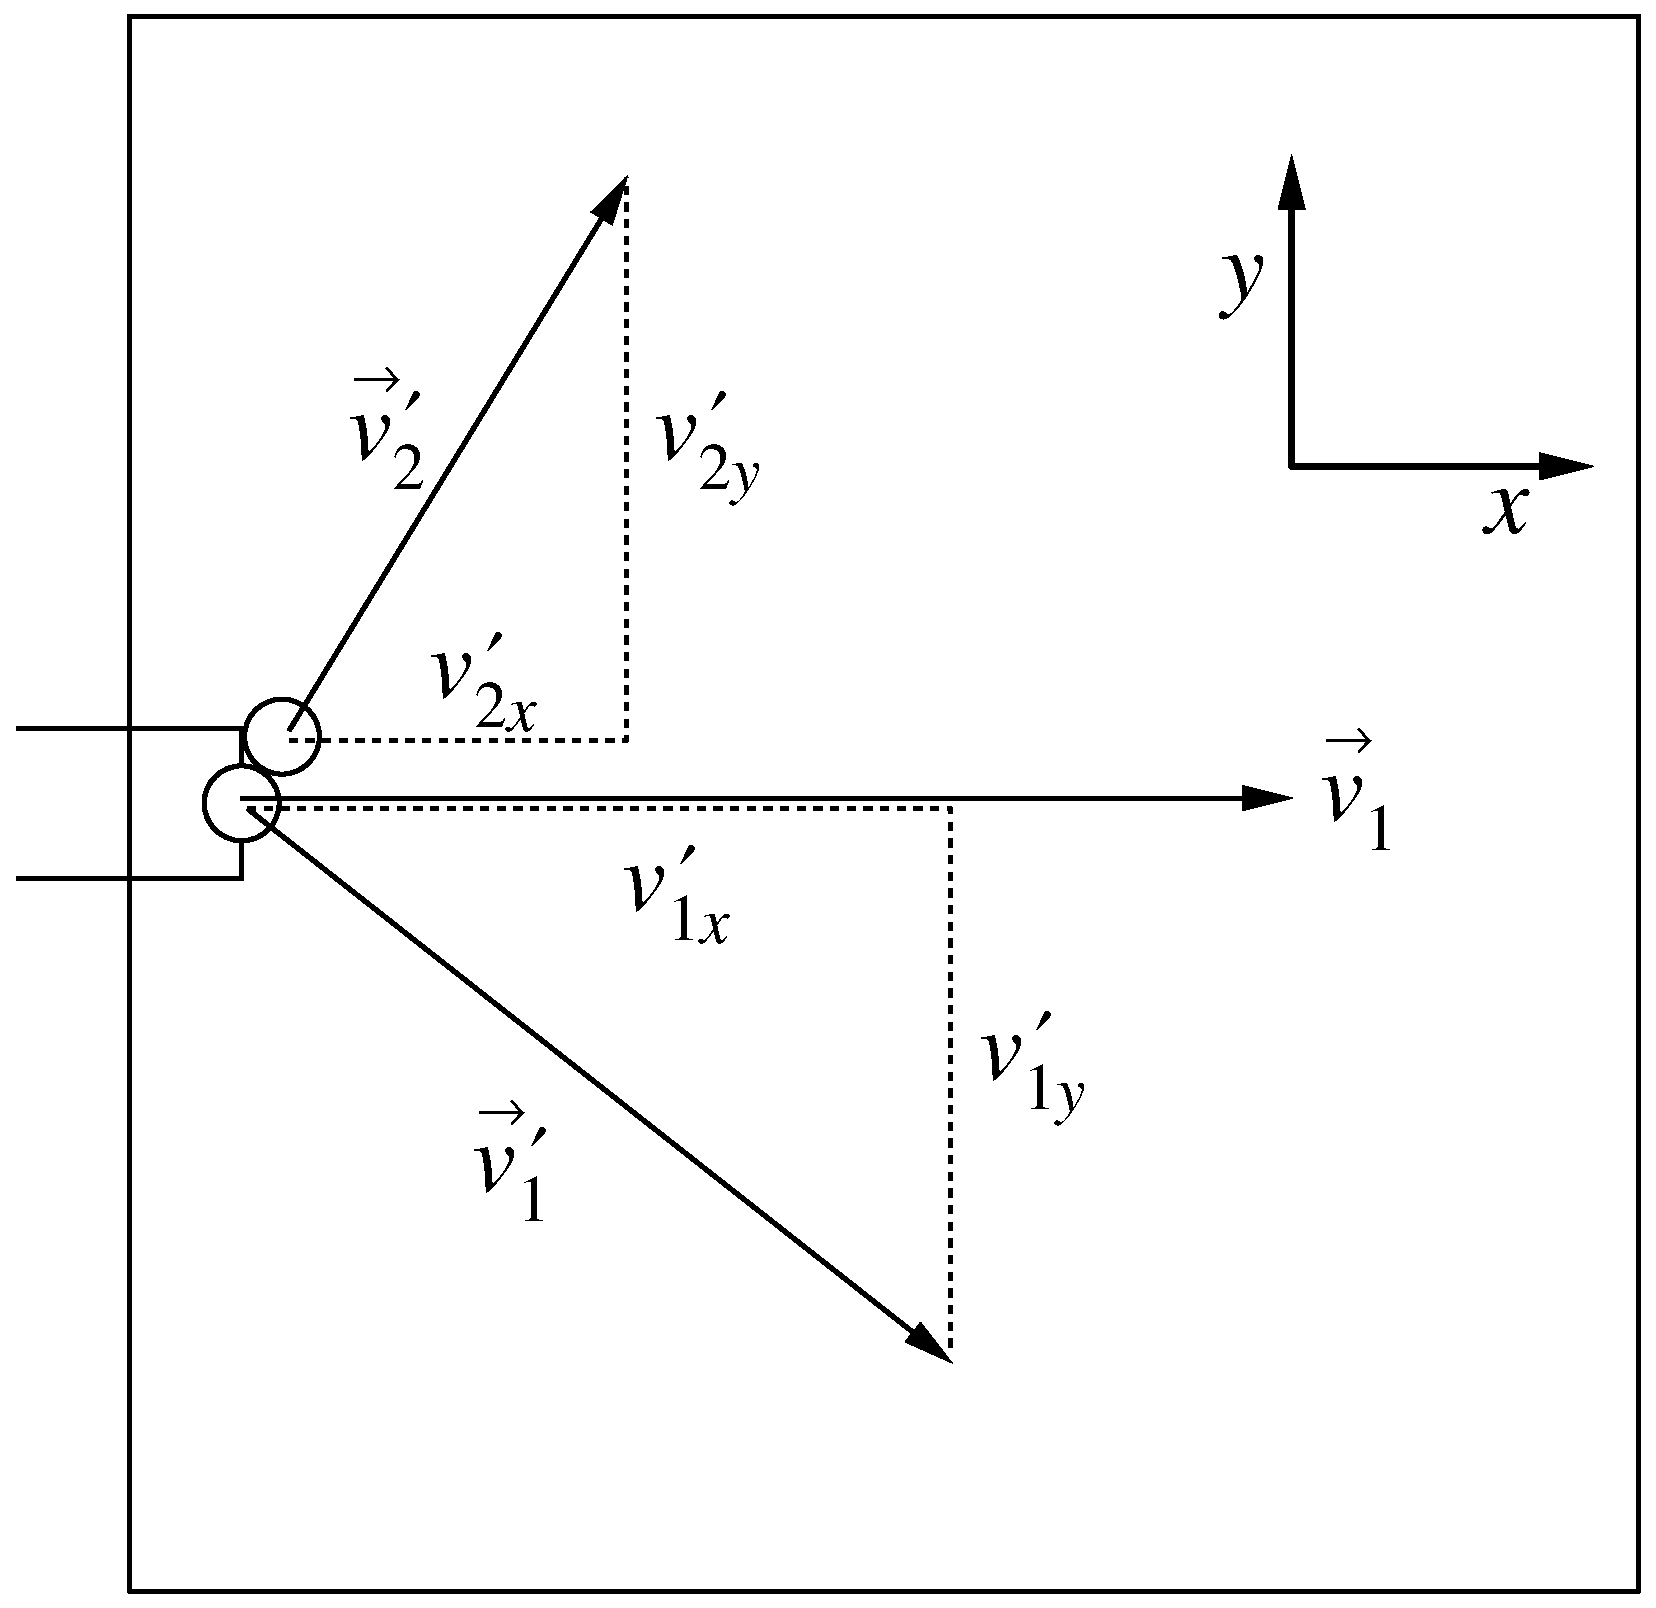
\includegraphics{2-body.coord.eps}}}}
\end{center}
%\vspace{3.375in}
%\special{ps:fig6_2.ps}
\caption{Coordinate system to be used in analyzing the data.  \label{fig:tb2}}
\end{figure}
     Using the coordinate system shown in Figure~\ref{fig:tb2} with origins
appropriate for the collision point, measure the $x$ and $y$ components
of each of the ball's velocity after the collision in units of cm/shake.  From
this information, calculate the components of the momentum for each ball
and the total momentum after the collision.  Again we can simplify
our calculations by inventing a new unit of mass, a {\em steely}, exactly
equal to the mass of the steel balls.  The
momentum vector (in units of ${\rm steely\cdot cm/shake}$) is
numerically equal to the $x$ and $y$ components of the displacement in cm.
The law of conservation of momentum now looks like a law of
conservation of the components of displacement.
Compare the $x$ and $y$ components of the total momentum
after the collision to the total momentum before the collision.  
Use Eq.~E.5 to find the error in each component of final total momentum. To what
accuracy do your measurements confirm that $P_{x}$ and $P_{y}$ are conserved
in the collision?

Use your velocity data to calculate the initial and final kinetic
energy of each ball (in units of ${\rm steely\cdot cm^2/shake^2}$).  Calculate the total initial
and final kinetic energy of the balls.  What percentage of energy is
lost to heat and sound during the collision?  (Note that percentage energy lost
contains no funny units [or any units at all], and hence is exactly the same
as what you would have calculated if you'd gone through the bother of using normal
units.)

It is possible to determine the mass of an object by observing the
effects of a collision of that object with an object of known mass and
velocity.  This is the method used by Chadwick to measure the mass of
the neutron in 1932.  Devise an experiment, based on conservation of
momentum principles to measure the mass of a marble. %Remember to adjust
%the holder height to make room for the larger marble.
To what accuracy does your experimental marble
mass agree with the measured mass of the marble?

\section*{Conclusions}
List all your numerical results and their uncertainties in a carefully
constructed table, and discuss them in detail.  For example, was momentum
conserved within the limits of experimental error?  Energy?
Comment on the amount of energy lost during the collision and on the
accuracy of your determination of the unknown mass.  Mention any sources of
error, both systematic and random.

\section*{Laboratory Report}
An acceptable laboratory report should include the following:
\begin{enumerate}
\item A brief description of your experimental procedure, including a diagram of the apparatus.
\item Table listing the measured components of momentum (with estimated errors).
\item A comparison of final and initial momentum with sample computations, listed by components (with estimated errors).
Did you confirm momentum conservation?
\item A calculation of percent kinetic energy lost (no error calculation required).
\item A description of your mass determination experiment.
\item A calculation of marble mass (no error calculation required) and comparison to actual mass.
\item Answers to all questions in the lab manual.
\item Calculation and discussion of experimental error.
\end{enumerate}

\section*{Critique of Lab}
     Follow the suggestions given in the Introduction to the
Laboratory Manual.

\section*{Quick Report Card}
Properly report (sigfigs, units, error) your values for $x$
momentum before and after the collision and your values for $y$
momentum before and after the collision.

%\renewcommand{\newname}{WORK DONE BY A VARIABLE FORCE}
%\include{variforce}
\renewcommand{\newname}{Rotational Dynamics}
%ROTATIONAL DYNAMICS
\newexp

%\begin{tabbing}
%references01234   \=   col2   \kill
%References: \> Pasco Rotational Dynamics Experiment Manual \\
%            \> Halliday, Resnick, and Walker, pp.\ 291--308
%\end{tabbing}

{\bf Apparatus:  }Pasco rotational dynamics equipment, including
\begin{enumerate}
\item A small unit having a digital display, a cylinder bearing, and a
spindle on which two steel disks are mounted.  {\em DO NOT remove these steel
disks}.  {\em DO NOT rotate the steel disks unless the air is on and at a minimum
of 9 psi (some units require 12 psi)}.
\item A small pulley, appropriate solid screws, one/two drop pins, an anchor washer connected to
a $25 \:$g mass by a piece of string, and a bar or large cylindrical ring (with plate).
\item An air regulator connected to the unit and a compressed air supply.
\item A lab computer with a Pasco interface and software for data analysis.
\item Calipers (accuracy: 0.02~mm)
\item Digital balance
\end{enumerate}


{\bf Note:  }This experiment is divided into two parts.  In the first
part you will measure
the moment of inertia (or rotational inertia) of a rigid body and
compare the result with theory. In the second
part you will investigate the law of conservation of angular momentum.

\begin{center}
{\Large {\bf Part I --- Rotational Inertia}}
\end{center}

\section*{Introduction and Theory}
The object of this experiment is to measure the moment of inertia of
a rigid body rotating about a fixed axis.  We will need
the rotational form of Newton's second law:
\begin{equation}
{\tau} = I {\alpha}  \label{eq:rot1}
\end{equation}
where ${\tau}$ is the torque, $I$ is the moment of inertia, and
${\alpha}$ is the angular acceleration.  In this experiment, we
will  apply a torque to  a rigid body
and measure the resulting
angular acceleration $\alpha$; and then use Eq.~\ref{eq:rot1} to
calculate the rotational inertia $I$.

Please examine Fig.~\ref{fig:rot1} carefully, particularly the side
view, and examine the apparatus itself when you come to lab.  You will
see two cylindrical steel disks, one on top of the other.  For this
part of the experiment, the bottom disk is fixed, and the top one is
allowed to rotate with minimal friction on an air cushion that we
set up between the two disks.

We exert a torque as follows:  wrap a string around a pulley that
is attached to the top disk.  The string goes over a second pulley
(Fig.~\ref{fig:rot1}, left end of the side view), where it is attached to a weight.  When
the weight is released, the tension in the string exerts a torque 
that
causes the top disk to rotate about its axis, as it floats on the
cushion of air.

If we calculate the torque, and use the Pasco apparatus to measure the
angular acceleration of the rotating disk, we can use
Eq.~\ref{eq:rot1} to find the rotational inertia of the rotating
system.

%To find the moment of inertia you will use Eq.~\ref{eq:rot1}.  You
%will apply a torque and measure the resulting angular acceleration.
%Actually the computer will take displacement vs.\ time data and calculate the
%angular acceleration for you, thus simplifying the task.

We can attach the object whose rotational inertia we want to measure
to the top disk.  Thus, we can find the rotational inertia of
this object as follows:
\begin{itemize}
\item Find the rotational inertia of system without the object.
%
\item Attach the object (either a cylindrical ring or a
rectangular bar) to the top disk and find the rotational inertia of
the combined system.
%
\item Subtract the second rotational inertia from the first to find
the rotational inertia of the object alone.
\end{itemize}
We can then compare the experimental value of $I$ to a theoretical
prediction based on the object's shape.

\begin{figure}     
\begin{center}
{\resizebox{4.5in}{!}{{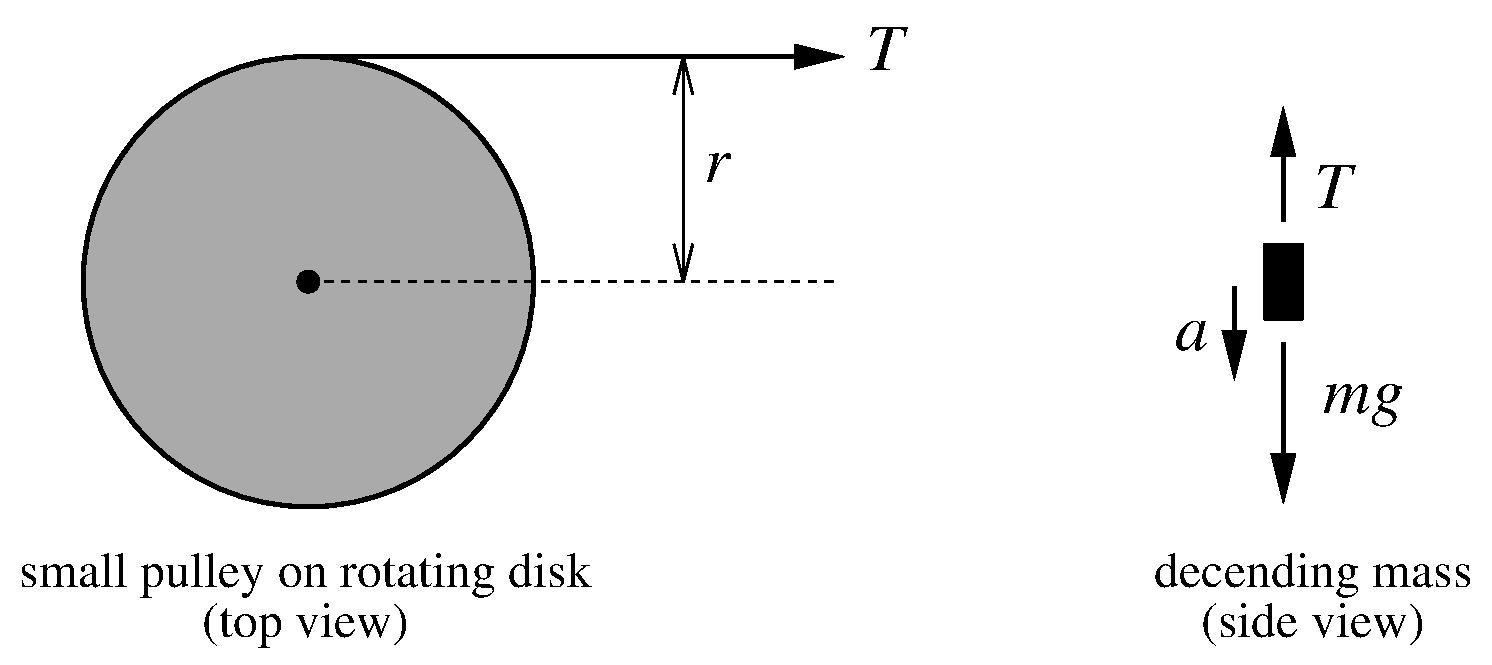
\includegraphics{freebody2.eps}}}}
\end{center}
%\vspace{3in}
%\special{eps:freebody.eps}
\caption{Force diagram for the rotational inertia apparatus.  The tension, $T$, in a thread wrapped around the
small pulley (radius: $r$) provides a torque that spins the system.  The tension in the thread
results from the force of
gravity, $mg$, on the descending mass.
The tension is slightly less than the force of gravity, so the descending mass has
a (small) acceleration, $a$.
          \label{fig:freebody}}
\end{figure}
%
\subsection*{Calculating the experimental rotational inertia}
\begin{figure}
\begin{center}
{\resizebox{4in}{!}{{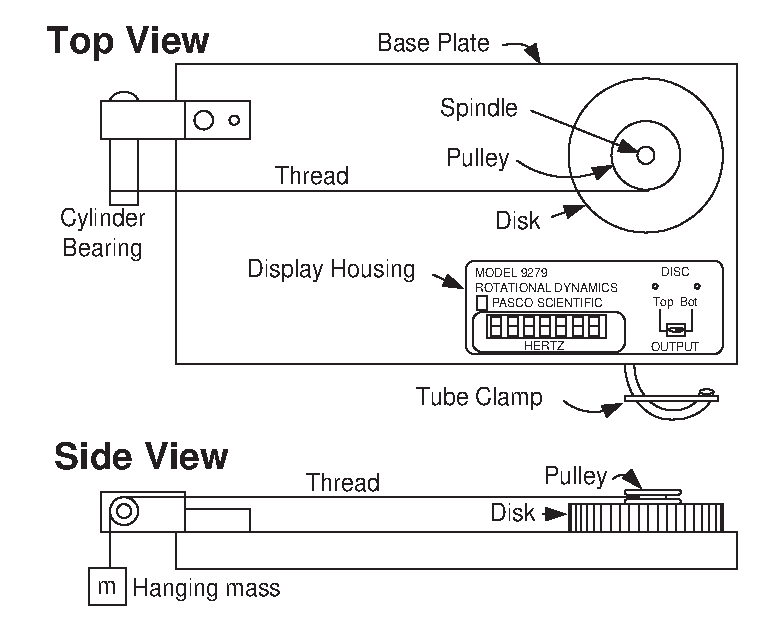
\includegraphics{Rotatefig.eps}}}}  %was diskB.eps
\end{center}
% \vskip.2in
% \vskip5.5in
% \special{bmp:disk.bmp y=5.5in}
 \caption{Rotational motion apparatus.  \label{fig:rot1}}
 \vskip.2in
\end{figure}

Consider the apparatus shown in Figures~\ref{fig:rot1} and
\ref{fig:rot2}.  We seek an expression for the rotational inertia
$I$ of the rotating system:  the rotating top disk with or without the object
(cylindrical ring or rectangular bar) placed on top of it.

First, we must find the torque that the string exerts on the top
disk.  The equation that relates torque to force is:
\begin{equation}
\vec{\tau} = \vec{r} \times \vec{F}
\end{equation}
where $\vec{F}$ is the force acting on the object, at a distance
$\vec{r}$ from
the axis of rotation.  Using the definition of the vector
product, we find that the magnitude of the torque can be written
\begin{equation}
\tau = rF \sin\theta
\end{equation}
where $\theta$ is the angle between $\vec{r}$ and $\vec{F}$.

As noted above, the torque is exerted by the
tension in a thread wrapped around a pulley.
Thus the force is the tension $T$ in the thread, and $r$ is the radius
of the pulley mounted on the top disk (see
Fig.~\ref{fig:freebody} and the right side of the side
view in  Fig.~\ref{fig:rot1}.)  Under these circumstances, the angle
$\theta$ will always be equal to $90^{\circ}$ making $\sin\theta = 1$.
Therefore, the torque on the system is
\begin{equation}
\tau = rT.
\end{equation}

To find an expression for the moment of inertia $I$ of the entire
system, we apply the rotational form of Newton's second law:
\begin{equation}
\tau = Tr = I \alpha.
\end{equation}
We also apply the linear form of Newton's second law to the
descending mass (choosing positive down):
\begin{equation}
mg -T = ma  \;\;\; {\rm or}
\end{equation}
\begin{equation}
mg -m \alpha r = T
\end{equation}
where we have used the usual relation between linear and angular acceleration,
$a=\alpha r$.  We combine these two equations to get the result
\begin{equation}
mgr = (I + mr^{2}) \alpha  .
\end{equation}
We could just solve this equation for $I$.  However, it will turn
out that the second term in the parentheses ($ mr^{2}$) is much smaller
than $I$. Consequently, to a very good approximation, we can neglect
this term.  If we do so, and solve for $I$, we obtain
\begin{equation}
I = {mgr \over \alpha}
\label{eq:rotfree}
\end{equation}


Equation E.10 then applies and 
the uncertainty in $I$ is given by
\begin{equation}
{\delta I \over I} = \sqrt{
                           \left( {\delta m \over m} \right)^2  +
                           \left( {\delta r \over r} \right)^2  +
                       \left( {{\delta \alpha} \over \alpha} \right)^2
                     }
\end{equation}
Be sure to include your derivation in your lab notebook.


\subsection*{Theoretical expressions for rotational inertia}

\paragraph*{cylindrical ring:}
The equation for the rotational inertia of a
cylindrical ring rotating about its axis is:
\begin{equation}
I = {{1} \over {2}} \, M \, \left( R_{\mbox{{\small out}}}^{2} +
    R_{\mbox{{\small in}}}^{2}
    \right)    \label{eq:rot2}
\end{equation}
where $M$ is the mass of the ring, $R_{\mbox{{\small out}}}$ is the
outer radius of
the cylinder, and $R_{\mbox{{\small in}}}$ is the inner radius.

The uncertainty is {\em approximately}:

%MathType!ZZhx47!eeaaduGcbmGdaaqacqizcGPasmysaeGedMeaaiGH9mqdaaqadeaaae
%WaoaaabiaHKjaMiiXGnbqasmytaaaacyjkcyzkamWdaaWcreGaikda
%aOGagUYabaaabiaIYmGdaaqacqizcGjcsmOud8qaaSqace4BceyDce
%iDaebaaOqasmOud8qaaSqace4BceyDceiDaebaaaaakiGLOiGLPaWa
%paaaleracGOmaaGccy4kdeaaaeGaikZaoaaabiaHKjaMiiXGsnWdba
%WcbiqGPjqGUbqeaaGcbiXGsnWdbaWcbiqGPjqGUbqeaaaaaOGawIIa
%wMcad8aaaSqebiaIYaaaaebaaaa!233A!
\begin{equation}
{{\delta \,I} \over I}=\sqrt {\left( {{{\delta \kern 1pt M} \over M}} \right)^2+\left( {2{{\delta \kern 1pt R_{out}} \over {R_{out}}}} \right)^2+\left( {2{{\delta \kern 1pt R_{in}} \over {R_{in}}}} \right)^2}
\end{equation}

\paragraph*{rectangular bar:}
The  equation for
the rotational inertia of a rectangular bar rotating about its center
of mass is: \begin{equation}
I = {{1} \over {12}} \, M \, \left( \ell^{2} + w^{2}  \right)
       \label{eq:rot3}
\end{equation}
where $M$ is the mass of the bar, $\ell$ is the length of the bar and $w$
is the width.

The uncertainty is {\em approximately}

%MathType!ZZhx47!eeaaduGcbmGdaaqacqizcGPasmysaeGedMeaaiGH9mqdaaqadeaaae
%WaoaaabiaHKjaMiiXGnbqasmytaaaacyjkcyzkamWdaaWcreGaikda
%aOGagUYabaaabiaIYmGdaaqacqizcGjccSiBaeGalYgaaaGawIIawM
%cad8aaaSqebiaIYaaakiGHRmqaaaqacGOmd4aaaeGaesMayIGedEha
%biXG3baaaiGLOiGLPaWapaaaleracGOmaaaaraaaaa!1944!
\begin{equation}
{{\delta \,I} \over I}=\sqrt {\left( {{{\delta \kern 1pt M} \over M}} \right)^2+\left( {2{{\delta \kern 1pt \ell } \over \ell }} \right)^2+\left( {2{{\delta \kern 1pt w} \over w}} \right)^2}
\end{equation}

%Be sure to include a derivation of the expression for the uncertainty
%in the theoretical value
%of whichever object you use, given the uncertainties in the measured
%quantities (mass and dimensions).   Use the methods developed in Appendix A.

\section*{Procedure}

%Before you begin, record in your lab notebook the masses and radii of the top
%and bottom steel disks. Label these quantities {\em clearly} so as not to
%confuse them with each other.  These quantities can be found on the base
%of the Rotational Dynamics unit.  Also record the radius of the pulley that
%you will use.  Measure its diameter using a caliper and divide this by two
%to get the radius.  You will need this quantity to calculate the applied torque.
%Also record the dimensions and mass of the square aluminum plate.

First check to make sure the unit is level by placing the bubble level
on the top steel disk.  The bubble should be centered in the level.
Then rotate the level $90^{\circ}$ and check the position of the
bubble again.  If it is not in the same position as before or is not
centered, the unit {\em may} need leveling --- ask your instructor to
examine your apparatus.  {\bf Note:} If the unit is not level, the
angular acceleration will not stay constant and your data may be
affected.

Once your unit is level, turn on the
air supply and adjust the regulator so that the air pressure is between 9 and 12 psi.
The air pressure is adjusted by turning the knob on top of the regulator.

Compressed air emerging from small nozzles in the base and
spindle form a cushion on which the top disk can float.  In
this way, friction is eliminated (or at least minimized).
The apparatus
uses an infrared detector to measure the passing of the light and dark bands on the
sides of the disk.  
%This quantity is shown in the display and has units of bands/sec or
%hertz (Hz).  
You can change which disk you are monitoring by toggling the
Top/Bottom switch.  
The wires emerging from the display box carry signals to
the computer so that the frequency of both the top and bottom disks can be
monitored simultaneously.  The Pasco software converts this signal
into angular velocity, so that one can measure the angular velocity of
the disk as a function of time.

On some units, there is a white tube clamp underneath the base of
the unit.  When it is closed, it allows the bottom disk to rotate freely on
the base.  When it is opened, the bottom disk will rest securely on the base.
Since we will only use the top disk in this part of the experiment, open the
tube clamp.  On other units this same function is controlled by a drop pin.

The top disk can be made to rotate freely on the bottom disk by plugging
the hole in the axle with a solid screw (or in Part II by filling
the hole with a drop pin)
%placing the drop pin or screwing a solid screw into the opening at the center
%of the disk.  
In this part of the experiment we will use the solid screw which must
thread the anchor washer (with attached string) and the pulley --- connecting both to the center of the top disk.
The anchor washer fits into the recess of
the pulley and the thread fits through the slot in the pulley.  The screw goes
through the hole in the square aluminum plate (if used, see Option A below), the pulley, the washer and into
the threaded hole in the top of the disk.  The thread comes out of the slot in
the pulley, runs over the groove in the cylinder bearing, and suspends the
falling mass.

In order for the mass supplying the torque to fall freely, place the apparatus
so that the cylinder bearing hangs over the edge of the table.
%Using the {\em solid, grey} screw secure the square aluminum plate
%(if needed---it is used only for the cylindrical ring), the thread
%anchor washer, and the small pulley to the hole in the center of the top disk.
\begin{figure}
\begin{center}
{\resizebox{4in}{!}{{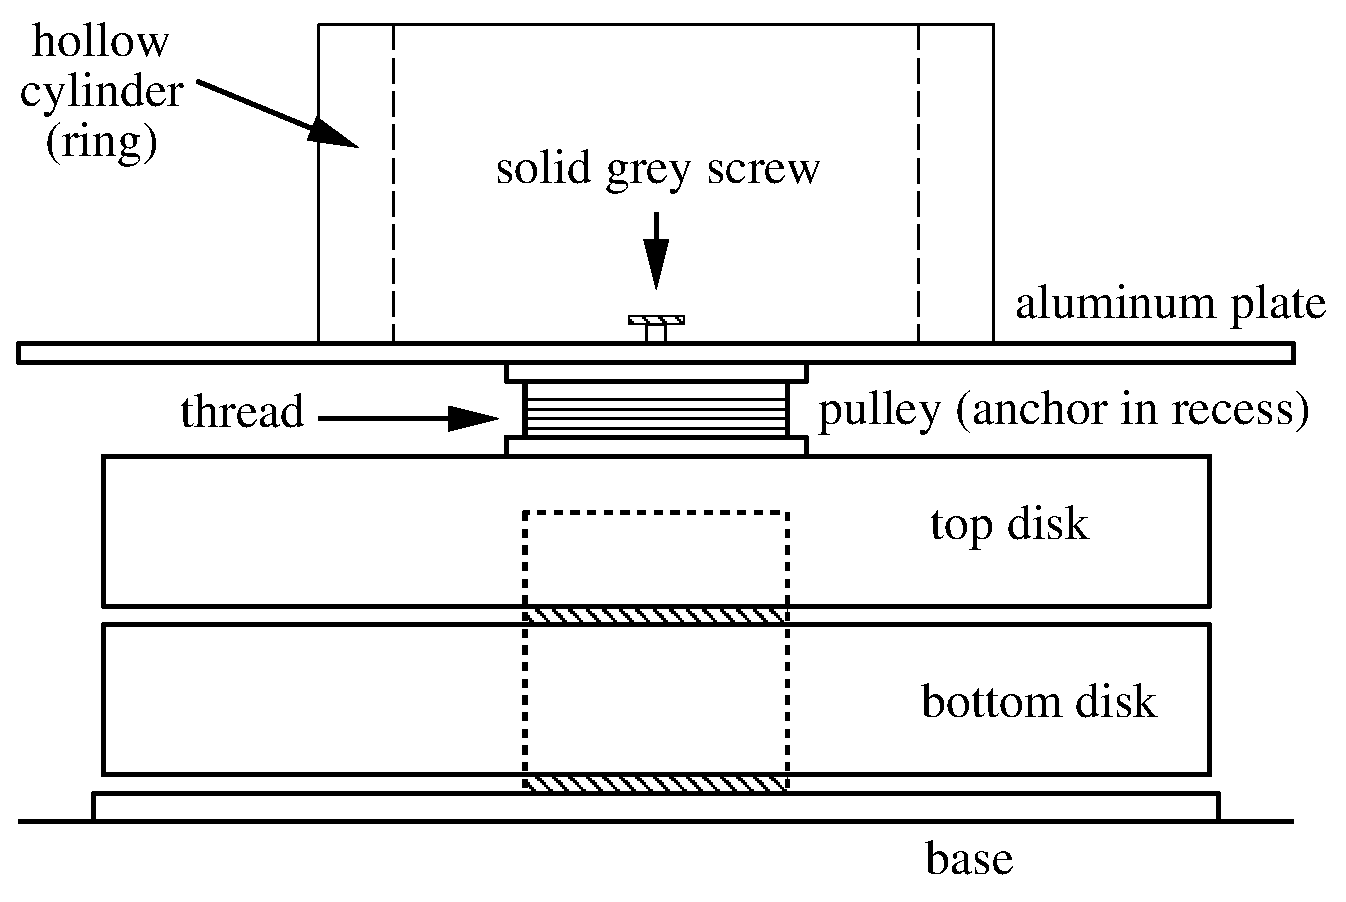
\includegraphics{plate.eps}}}}
\end{center}
%\vspace{2.75in}
%\special{bmp:plate.bmp x=5.5in y=2.75in}
\caption{Diagram for setting up the Moment of Inertia experiment.
  \label{fig:rot2}}
\end{figure}
See Figure~\ref{fig:rot2}.  

Now check to make sure that the air pressure is still at the right value for
your set-up (keep
monitoring the pressure throughout the experiment).  The bottom disk should be
stable (the tube clamp is open, or drop pin out) and the top disk should rotate freely.  By
{\em gently} turning the top disk, wind the thread around the pulley until the
top of the descending mass is level with the bottom of the cylinder
bearing
bracket.  Hold the top disk stationary for a moment and then release it, being
careful not to impart any initial angular velocity to the disk.  The falling
mass should accelerate the disk.  The thread should unwind from the pulley
and, before the mass hits the ground, the thread should begin to start winding
back on the pulley.  If the mass does hit the ground, shorten the length of
thread appropriately.  Make a couple of test runs to get used
to the equipment.  %Make sure the switch on the display housing is in the `TOP'
%position since only the top disk is rotating.

{\bf Note:  Observe a short ``mini" experiment on conservation of
energy at this point.}  After you drop the mass as outlined above, it
will reach its minimum point, and then rise again as the kinetic
energy of the disk is transferred back into the potential energy of
the small mass $m$.  See how near the mass gets to its original
starting position---very little energy is lost to friction in
this process.

%The next step is to get acquainted with the computer and software.
%You will be given a handout that describes, in detail, the steps to use
%the IBM PC and Pasco Interface for taking data.

%A couple of things to remember are:
%\begin{enumerate}
%\item Fifteen data points are sufficient.
%\item The number of dark bands per revolution is {\bf 200}.  Entering this value
%allows the program to convert the units from bands/sec to radians/sec.
%\item The number of dark bands per data point is {\bf 50}.  Entering this value
%tells the computer to measure the time it takes for 50 bands to pass the sensor.
%\end{enumerate}
%After entering the quantities enumerated above, the program will prompt you with
%\begin{verbatim}
%PREPARE TO RELEASE OBJECT
%PRESS ANY KEY TO CONTINUE
%\end{verbatim}
At this point wind up the thread and hold the disk steady.
Tell the Pasco
software to begin taking data, and then release top disk
plate {\em without imparting any initial angular velocity to it}.

%The computer will pause for a while for data taking and calculations.  When it
%is done with its calculations it will display information regarding the run on
%the screen.  {\em Copy down the value of the acceleration in your notebook}.
%You can view the displacement vs.\ time graph if you want, but {\em definitely}
%view the velocity vs.\ time graph.

Check the angular velocity vs.\ time graph to make
sure that it is a linearly increasing function of time. Continue until two
complete up-and-down cycles have been recorded and then hit Stop. Select a
linear portion of the data, and transfer it to \WAPP.  (Use $\delta \omega = .03$~rad/sec
and neglegible error in time.) Do a
least-squares fit to find the angular acceleration (the slope of the
graph of angular velocity vs. time).  You don't need to print the fit
report, but do be sure to record the angular acceleration in a data
table.

If your graph of angular velocity vs.\ time appears to be okay, continue to take three
more measurements of angular acceleration and record the absolute value of four values 
(two from up segments, two from down segments) in your
lab notebook in a data table.  When you analyze the data you will average the
four (now positive) angular accelerations and use the average acceleration to
calculate the moment of
inertia of the setup (i.e., the aluminum plate (if used), the pulley, and the
top disk).  The standard deviation of the mean\footnote{
Recall: see page \pageref{sdev.mean} or  \pageref{atwood.sdev.mean}.} will be the uncertainty
in the angular acceleration ($\delta\alpha$).

Our strategy will be to measure
the rotational inertia of the system with and without an object.  The
rotational inertia of the object alone will then be the difference
between these two values.  We have just measured the angular acceleration
without an object, so we must next:
%
\begin{itemize}
\item Measure the angular velocity as a function of time for
the system with the object.
%
\item Paste the angular velocity vs.\ time data into \WAPP, and do a
least-squares fit to find the angular acceleration.
%
\item Repeat the procedure outlined above, recording
four measurements of angular acceleration in a table. Calculate the
average angular acceleration and the standard deviation of the mean
($\delta \alpha$) just as you did before but now with the object aboard.
\end{itemize}

{\bf Select an object, add it to the system and measure the angular acceleration!}

\subsubsection*{Option A:  Rotational inertia of a cylindrical ring}
%Now you are ready to measure the moment of inertia of a cylindrical
%ring. 
Take either of
the two black, steel cylindrical rings and measure its mass and the
inner and outer diameters. Record these values in your
lab notebook.

The cylindrical ring is mounted on an aluminum plate, which will be
clamped to the top steel disk with the pulley between---your instructor will show you how.
Make sure to fit the locating pins on the ring into the holes
in the aluminum plate, so that the cylinder will rotate about its
center of mass.

\subsubsection*{Option B: Rotational Inertia of a Solid Rectangular
Bar} The procedure is similar to the one outlined above, except that
we will not need the aluminum plate.  First, record the
mass and dimensions of the rectangular steel bar in your lab notebook.

Secure the bar on top of the pulley (which is on top of the steel disk)
with the {\em solid, red}
screw.  The {\em red} screw will go through the bar, the pulley, the
thread
washer, and into the steel disk.

\section*{Data Reduction and Analysis}

For whichever object you used, you should have average angular
accelerations (with error) for the system with
and without the object.  To find the moment of inertia of the object
alone, proceed as follows:

\begin{enumerate}
%\item
%Collect your average accelerations in a table, along with their
%uncertainties.
%
%\item Find the torque exerted on the system by the descending mass,
%using the equations derived above.
%
\item Use Eq.~\ref{eq:rotfree} above to find the both rotational
inertias (with and without the object).
%
\item Find the uncertainty in both rotational inertias.
%
\item Subtract your experimental rotational inertias to find the rotational inertia of the object alone,
and calculate its uncertainty (see page \pageref{table1} or Appendix E).
%
\item Finally, calculate the theoretical value of the rotational
inertia, with uncertainty, and compare it with your experimental
result.
\end{enumerate}
Summarize your results in a carefully constructed table.

%Calculate the applied torque by multiplying the force ($F = mg$, where
%$m = 25\:$g and $g=980\:$g-cm/s$^{2}$) by the radius of the pulley.  This will
%give you the torque in units of g-cm$^{2}$/s$^{2}$.  When this torque is divided
%by the angular acceleration, you will get the moment of inertia in units of
%g-cm$^{2}$.
%
%Next find the average of the angular accelerations for your three sets of data
%(i.e., aluminum plate only, aluminum plate plus cylinder, and aluminum plate
%plus rectangular steel
%bar).  Also find the uncertainty in this average; the uncertainty will be the
%standard deviation of your five values.  Record these as
%$\bar{\alpha} \pm \sigma_{\alpha}$ where
%$\bar{\alpha} = \alpha_{\mbox{{\small average}}}$
%and $\sigma_{\alpha}$ is the standard deviation of your five values.
%
%Using your aluminum-plate-only data, calculate the moment of inertia of the
%aluminum plate plus top disk by dividing the torque by the average acceleration.
%Also record the uncertainty in this moment of inertia.  The moment of inertia of
%this system will be subtracted from the moments of inertia of the other two
%systems to find $I_{\mbox{{\small cyl}}}$ and $I_{\mbox{{\small bar}}}$.
%
%Using your aluminum plate plus cylinder data, find the moment of inertia of
%this system.  To get the moment of inertia of the cylinder only, subtract off
%the moment of inertia of the top disk/aluminum plate system.  Make sure you
%calculate the uncertainty associated with this value.  Also calculate
%the moment of inertia of the cylinder using mass amd dimension data and
%Eq.~\ref{eq:rot2}.  Compare these two values.  Are they in agreement?
%
%Using your aluminum plate plus rectangular steel bar data, find the moment of
%inertia of this system.  To get the moment of inertia of the bar only, subtract
%off the moment of inertia of the top disk/aluminum plate system.  Make sure you
%calculate the uncertainty associated with this value.  Also calculate
%the moment of inertia of the bar using mass and dimension data and
%Eq.~\ref{eq:rot3}.  Compare these two values.  Are they in agreement?

\begin{center}
{\Large {\bf Part II --- Conservation of Angular Momentum}}
\end{center}
\section*{Introduction}
Angular momentum, $\vec{L}$, can be written as the product of the moment of inertia,
$I$, and the angular velocity, $\vec{\omega}$. (Please see your
textbook for a more complete discussion.) In this experiment we will
see whether or not angular momentum is conserved.

The experiment works as follows:  We will set up the apparatus so that
{\em both} disks can rotate independently, and set them rotating at different
angular velocities, ${\omega}_1$ and ${\omega}_2$ (and thus with different
initial angular
momentum, ${L}_1$ and ${L}_2$).  Then, we collapse the air cushion between the two disks, so
that they come together and rotate {\em as a single body}, with some
final angular velocity ${\omega}_f$ and angular momentum ${L}_f$.  We can then
compare the initial and final angular momenta and see if
angular momentum is conserved:
\begin{eqnarray}
L_f &=& L_1+L_2 \label{eq:Lconserved1}\\
I_f \omega_f &=& I_1\omega_1+I_2\omega_2 \label{eq:Lconserved2}\\
{1\over2}M_f R^2 \omega_f &=& {1\over2}M_1 R^2\omega_1+{1\over2}M_2 R^2\omega_2 \label{eq:Lconserved3}\\
M_f  \omega_f &=& M_1 \omega_1+M_2 \omega_2 \label{eq:Lconserved4}
\end{eqnarray}
In this final form, conservation of angular momentum looks exactly like
conservation of linear momentum!

Remember that in such a `totally inelastic' collision, kinetic energy is not
conserved.  We can check by calculating the initial and
final kinetic energies.  %What would you expect, given the problems we
%have solved in class?

The computer will graph the angular velocities of the
two disks before, during and after the collision, allowing  you to select the initial and final
angular velocities.  %From these angular velocities you will calculate the
%initial and final angular momenta and kinetic energies.

\section*{Procedure}
Begin by closing the white tube clamp located underneath the base of the unit or
inserting the drop pin into the labeled valve.
Doing so will allow the bottom disk to rotate freely.

Record the masses %and radii 
of the top and bottom disks.%---these values will
%be supplied by your TA.  You will use
%them later to calculate the moments of inertia for the top and bottom disks.

Insert the ``drop pin'' in the hole in the top disk's axle, so that the top
disk will rotate independently of the bottom one.  (Your instructor
will show you how.) Spin the bottom disk fairly fast and the top disk
more slowly.  Spin the two disks in the {\em same direction}.  {\em
You must make sure that both disks have some initial angular
velocity}.

Tell the computer to start taking data.  Let it record the initial
angular velocities for several seconds, and then collapse the air
cushion by pulling the drop pin.  Stop the data collection a few
seconds after the collision when the disks are rotating as one.
%
%The Pasco DataStudio program will then display
Select from the resulting graph (a bit just before or after the collision)
the initial ($\omega_{1}$ and $\omega_{2}$) and final ($\omega_{f}$)
angular velocities. (If you select the $\Sigma$ button on the graph it
will display the mean $\omega$ for the data you select.)


%Run the experiment four times in all and collect you data in a table.
%Leave
%eight columns for the following quantities: initial angular momenta for the top
%and bottom disks, initial rotational kinetic energies for the top and bottom
%disks, final angular momentum for the two disks together, the final
%rotational kinetic energy for the two disks together, the change in angular
%momentum, and the change in rotational kinetic energy.

\section*{Analysis}
%---OUT---
\begin{comment}
First calculate the moments of inertia for the top and bottom disks using the
equation
\begin{equation}
I = {{1} \over {2}} \, MR^{2}.
\end{equation}
The moment of inertia for the combined top/bottom disk situation will just be
the sum of the individual moments of inertia.

Next start filling in the table mentioned above for each of the four runs.
The angular momentum is equal to
\begin{equation}
\vec{L} = I \vec{\omega}.
\end{equation}
If you spun both disks in the same direction as outlined above, you
can ignore the vector nature of this equation.  If you spun
the disks in opposite directions, the angular momentum of one disk
will be negative with respect to the other.  It doesn't matter which
one you call negative.

The rotational kinetic energy is equal to
\begin{equation}
K_{\mbox{{\small rot}}} = {{1} \over {2}} \, I \omega^{2}
\end{equation}

Next calculate change in angular momentum from the initial to the final state:
\begin{equation}
\Delta L = L_{1} + L_{2} - L_{3}
\end{equation}
where $L_{1}$ and $L_{2}$ are the initial angular momenta and $L_{3}$ is the
final angular momentum.  Record $\Delta L$ for the four runs in tabular form.
The percentage of angular momentum lost can be calculated from:
\begin{equation}
{{\Delta L} \over {L_{1} + L_{2}}}
\end{equation}
Also calculate the change in rotational kinetic energy:
\begin{equation}
\Delta K_{\mbox{{\small rot}}} = K_{1} + K_{2} - K_{3}
\end{equation}
where $K_{1}$ and $K_{2}$ are the initial rotational kinetic
energies and $K_{3}$ is the final rotational kinetic energy.  Record
$\Delta K_{\mbox{{\small rot}}}$ for the four runs in tabular form.
The percentage of energy lost can be calculated from:
\begin{equation}
{{\Delta K_{\mbox{{\small rot}}}} \over {K_{1} + K_{2}}}
\end{equation}
\end{comment}
%---END OUT---------
Conservation of angular momentum says the change in
angular momentum should be be zero:
\begin{equation}
\Delta L \equiv L_{f} -(L_{1} + L_{2})=0
\end{equation}
As shown above, because the disks have the same radius, this can be simplified to:
\begin{equation}
M_1 \omega_1+M_2 \omega_2 -M_f  \omega_f = 0\label{eq:Lconserved5}
\end{equation}
Of course, because of measurement uncertainty, it will not be exactly zero,
so the question becomes: is it consistent with zero when errors are considered?

Using Eq.~E.7 we find the error in a product $M\omega$ is given by:
\begin{equation}
\delta(M\omega)=\sqrt{(M\delta \omega)^2+(\omega\delta M)^2}
\end{equation}
Using Eq.~E.5 we find the error in the sum (or difference) of such terms in
Eq.~\ref{eq:Lconserved5} is given by:
\begin{equation}
\sqrt{\left(\delta(M_1 \omega_1)\right)^2+\left(\delta(M_2 \omega_2)\right)^2+\left(\delta(M_f \omega_f)\right)^2}
\end{equation}
which expands to
\begin{equation}
\sqrt{(M_1\delta \omega)^2+(\omega_1\delta M)^2+(M_2\delta \omega)^2+(\omega_2\delta M)^2+(M_f\delta \omega)^2+(\omega_f\delta M_f)^2}
\end{equation}

Use a spreadsheet to make this calculation easier! Note: for this process we estimate the
error in the measurement of angular velocity to be:
\begin{equation}
\delta\omega = 0.1\mbox{ rad/sec}
\end{equation}

\section*{Conclusions}
\subsection*{Part I}
Present the results obtained in Parts I of the experiment in a
carefully constructed table.  Be sure to include uncertainties and units.

Your discussion of the results should include (but is not limited to)
the following points:
\begin{itemize}
\item Comment on the agreement between the experimentally determined
and the
theoretical values for the moments of inertia in Part I.  Do they
agree within experimental uncertainty?  What are the sources of error?
%Are there any
%rotating bodies that we did not take into account?  If so, would they affect
%the outcome of the experiment significantly?
\item Were we quantitatively justified in neglecting the $mr^2$ term
when we derived Eq.~\ref{eq:rotfree}?  Do a quick calculation to
justify your answer.
\end{itemize}

\subsection*{Part II}
Present the results obtained in Part II of the experiment in a
carefully constructed table.
Comment on the extent to which angular momentum was conserved.
Angular momentum is  conserved only if there are no {\em
external}
torques acting on the system.  If your results show that the angular momentum
of the system was not conserved, could it be due to the presence of an
external torque or is it merely the effect of experimental
uncertainty?

%Was the rotational
%kinetic energy conserved?  Does this tell you that the collision was elastic
%or inelastic?

\section*{Critique}
Follow the suggestions in the Introduction to the Laboratory Manual.

\section*{Quick Report Card}
Properly report (sigfigs, units, error) your experimental value for the object's $I$.
Properly report (sigfigs, units, error) your theoretical value for the object's $I$.

From Part II, properly report (sigfigs, units, error) $\Delta L$, i.e., Eq.~\ref{eq:Lconserved5}.
\renewcommand{\newname}{Simple Harmonic Motion}
%SIMPLE HARMONIC MOTION
\newexp
\section*{Introduction}
     In this experiment we will examine the behavior of a simple 
harmonic oscillator, that is, a mass attached to the end of a 
spring.  Remarkably, this system is one of the most important 
in all of physics.  Almost any problem that involves 
oscillations --- for example, the electrical oscillations in a 
radio, or the oscillations of an atom around a lattice site in a 
crystal --- can at least be approximated by the simple harmonic 
oscillator.

\section*{Analysis}
     As you may know from the lectures and textbook, Hooke's law 
states that the force exerted by a spring on a mass is given by
\begin{equation}
F = - kx   \label{eq:harm1}
\end{equation}
where $x$ is the displacement of the spring from its equilibrium 
position and $k$, called the spring constant, is a constant 
of proportionality that depends on the stiffness of the spring.

     We will attempt to measure the spring constant in two ways.  
In the first part of the experiment, we will hang masses on the 
spring, and measure the displacement from equilibrium for a 
number of different masses.  When the mass is at rest the 
gravitational force $mg$ will just balance the force exerted by the 
spring.  Hence a graph of force vs.\ displacement should allow you 
either to confirm or reject Eq.~\ref{eq:harm1}, and if the graph is a 
straight line, to determine the value of $k$ from a computer fit.

     In the second part of the experiment we will set the mass 
oscillating, and measure the period of oscillation, $T$ (that is, the 
time for one complete oscillation) as a function of mass.  Then, 
you can use your knowledge of graphical and computer analysis to 
find the functional relationship between period and mass.  Look 
up the theoretical expression for this relationship and use it 
along with your computer analysis to find a value for the spring 
constant $k$.  See if $k$ determined in this way agrees, within the 
limits of experimental uncertainty, with the value you found in 
the first part of the experiment.

\section*{Experimental Procedure}
     Examine the apparatus carefully and work out a suitable 
procedure for the experiment.  Keep in mind the following points:
\begin{enumerate}
\item Be sure you measure the mass of the weight holder, and add
it to your experimental masses.  You need the {\bf total} mass to
calculate the force on the spring!

\item Be sure you adjust the wire pointer on the apparatus to 
         eliminate the effects of parallax.
\item The largest source of experimental uncertainty in the 
         measurement of the period is in deciding exactly when to 
         start your timer, and exactly when to stop it.  The 
         effect of this error can be minimized by measuring the 
         time for a large number of oscillations.
\end{enumerate}
    
\section*{Analysis of Data}
     {\bf NOTE:}  Please be sure that you know what your units are, and
     that you are using units consistently, in the following
     analysis.

     Use the methods of graphical and computer analysis to find:
\begin{enumerate}     
\item The value of the spring constant $k$, using Hooke's law.  Be sure
that you also report the uncertainty in $k$, based on your least-squares
fit.

\item The functional dependence of the period of oscillation 
         on the mass.  Check your textbook, and compare your
	   result to the theoretical result. 
 
\item The value of the spring constant $k$, using your 
         oscillation data and analysis.  See if your two values 
         of the spring constant agree within the limits of 
         experimental uncertainty.  {\bf Note:}  This part is tricky
	   and you may need to consult your instructor.  Don't leave this
	   part until the last moment!
\end{enumerate}

\section*{Questions}
\begin{enumerate}
\item How could you find the velocity of the oscillating mass 
         at any arbitrary value of the displacement $x$?
\end{enumerate}

\section*{Conclusions}
Make a table listing all your numerical results and their uncertainties.
Comment on the consistency of your results for the determination of $k$ from
the two different methods.  Mention any sources of error, both
systematic and random.  Attach the fit results and plots as usual.

\section*{Critique of Lab}
     Follow the suggestions given in the Introduction to the
Laboratory Manual.

\renewcommand{\newname}{The Pendulum}
%THE PENDULUM
\newexp

       This experiment is, among other things, an exercise that
 allows you to devise your own experimental procedure and method
 of data analysis.

       You will be given a timer, a length of cord, a weight, and
 some clamps and assorted hardware.  Using this equipment, find
 how the period of a pendulum depends on its length.

       After you have finished this part, do a theoretical
 analysis of the pendulum, using your text if necessary, and use
 your results to find $g$, the acceleration of gravity.  Include a
 discussion of experimental uncertainty.

       Your writeup should include a detailed description of your
 experimental procedure, and a discussion of how you applied the
 techniques of graphical and computer analysis to your data.

%\renewcommand{\newname}{Kater Pendulum}
%% Kater Pendulum
\newexp

\section*{Introduction}

It is well-known result that the period T of a simple pendulum is given by
% MathType!MTEF!2!1!+-
% feaaeaart1ev0aaatCvAUfKttLearuavP1wzZbItLDhis9wBH5garm
% Wu51MyVXgaruWqVvNCPvMCG4uz3bWemv3yPrwynfgDOLeDHXwAJbqe
% gWuDJLgzHbIqYL2zOrhinfgDObss0fgBPngarqqtubsr4rNCHbGeaG
% qiVCI8FfYJH8sipiYdHaVhbbf9v8qqaqFr0xc9pk0xbba9q8WqFfea
% Y-biLkVcLq-JHqpepeea0-as0Fb9pgeaYRXxe9vr0-vr0-vqpWqaae
% aabiGaciaacaqabeaadaabauaaaOqaaiabdsfaujabg2da9iabikda
% Yiabec8aWnaakaaabaWaaSaaaeaacqWGmbataeaacqWGNbWzaaaale
% qaaaaa!46A8!
\[
T = 2\pi \sqrt {\frac{L}{g}} 
\]
where $L$ is the length.  In principle, then, a pendulum could be used
to measure $g$,  the acceleration of gravity.  However, practical
difficulties-primarily in measuring the length accurately-make it
unsatisfactory for high precision measurements.

It turns out that a physical pendulum-typically, a mass suspended from
a knife edge-can be used for much more accurate measurements.  The
Kater pendulum is such a physical pendulum.  It is named after its
inventor, Captain Henry Kater, a captain in the British army and a
Fellow of the Royal Society, who invented it around 1820.  For many
years, it was the standard method of measuring $g$ to high accuracy.

\begin{figure}[!hbt]     %Kater pendulum drawing, kater.eps
\vspace{3in}
\special{eps:kater.eps}
\caption{Kater Pendulum.  The pendulum can oscillate about a knife edge through either hole.  The holes are located so that the two periods of oscillation are nearly equal. \label{fig:kater}}
\end{figure}

The beauty of this experiment is that it allows us, using relatively
simple apparatus, to measure a physical quantity very accurately
indeed-we hope, to within a few parts in 10,000.  It works as follows:
Consider a physical pendulum with two supports that lie along a line
through the center of mass, as shown in Figure 1.

Suppose the distances $d_1$ and $d_2$ are adjusted so that the periods
around both supports are equal: 
$%\[
T_1  = T_2  = T
$%\]
  .  Then it can be shown that this
period is the period of a simple pendulum with length $L$ , the distance
between the supports.  Thus, if the period and that distance can both
be measured accurately, one can find the acceleration of gravity:
% MathType!MTEF!2!1!+-
% feaaeaart1ev0aaatCvAUfKttLearuavP1wzZbItLDhis9wBH5garm
% Wu51MyVXgaruWqVvNCPvMCG4uz3bWemv3yPrwynfgDOLeDHXwAJbqe
% gWuDJLgzHbIqYL2zOrhinfgDObss0fgBPngarqqtubsr4rNCHbGeaG
% qiVCI8FfYJH8sipiYdHaVhbbf9v8qqaqFr0xc9pk0xbba9q8WqFfea
% Y-biLkVcLq-JHqpepeea0-as0Fb9pgeaYRXxe9vr0-vr0-vqpWqaae
% aabiGaciaacaqabeaadaabauaaaOqaaiabdsfaujabg2da9iabikda
% Yiabec8aWnaakaaabaWaaSaaaeaacqWGKbazdaWgaaWcbaGaeGymae
% dabeaakiabgUcaRiabdsgaKnaaBaaaleaacqaIYaGmaeqaaaGcbaGa
% em4zaCgaaaWcbeaakiaaywW7cqqGVbWBcqqGYbGCcaaMf8Uaeeiiaa
% Iaem4zaCMaeyypa0ZaaSaaaeaacqaI0aancqaHapaCdaahaaWcbeqa
% aiabikdaYaaakmaabmaabaGaemizaq2aaSbaaSqaaiabigdaXaqaba
% GccqGHRaWkcqWGKbazdaWgaaWcbaGaeGOmaidabeaaaOGaayjkaiaa
% wMcaaaqaaiabdsfaunaaCaaaleqabaGaeGOmaidaaaaaaaa!620A!
\begin{equation}%\[
T = 2\pi \sqrt {\frac{{d_1  + d_2 }}{g}} \quad {\rm or}\quad {\rm  }g = \frac{{4\pi ^2 \left( {d_1  + d_2 } \right)}}{{T^2 }}
 \label{eq:kater1}
\end{equation}%\]

\section*{Theory}

In this section, we give a detailed derivation of Equation~(\ref{eq:kater1}).  The period of a physical pendulum is

% MathType!MTEF!2!1!+-
% feaaeaart1ev0aaatCvAUfKttLearuavP1wzZbItLDhis9wBH5garm
% Wu51MyVXgaruWqVvNCPvMCG4uz3bWemv3yPrwynfgDOLeDHXwAJbqe
% gWuDJLgzHbIqYL2zOrhinfgDObss0fgBPngarqqtubsr4rNCHbGeaG
% qiVCI8FfYJH8sipiYdHaVhbbf9v8qqaqFr0xc9pk0xbba9q8WqFfea
% Y-biLkVcLq-JHqpepeea0-as0Fb9pgeaYRXxe9vr0-vr0-vqpWqaae
% aabiGaciaacaqabeaadaabauaaaOqaaiabdsfaujabg2da9iabikda
% Yiabec8aWnaakaaabaWaaSaaaeaacqWGjbqsaeaacqWGnbqtcqWGNb
% WzcqWGKbazaaaaleqaaaaa!4916!
\[
T = 2\pi \sqrt {\frac{I}{{Mgd}}} 
\]

where $I$ is the moment of inertia about the axis of rotation 
of the pendulum, and $d$ is the distance from the axis of rotation to the center of mass.  From the Parallel Axis Theorem, it is apparent 
that

% MathType!MTEF!2!1!+-
% feaaeaart1ev0aaatCvAUfKttLearuavP1wzZbItLDhis9wBH5garm
% Wu51MyVXgaruWqVvNCPvMCG4uz3bWemv3yPrwynfgDOLeDHXwAJbqe
% gWuDJLgzHbIqYL2zOrhinfgDObss0fgBPngarqqtubsr4rNCHbGeaG
% qiVCI8FfYJH8sipiYdHaVhbbf9v8qqaqFr0xc9pk0xbba9q8WqFfea
% Y-biLkVcLq-JHqpepeea0-as0Fb9pgeaYRXxe9vr0-vr0-vqpWqaae
% aabiGaciaacaqabeaadaabauaaaOqaaiabdMeajjabg2da9iabdMea
% jnaaBaaaleaacqWGJbWyaeqaaOGaey4kaSIaemyta0Kaemizaq2aaW
% baaSqabeaacqaIYaGmaaaaaa!4855!
\[
I = I_c  + Md^2 
\]
where $I_c$ is the moment of inertia about the center of mass.  
Thus for our physical pendulum in Figure 1, we have

% MathType!MTEF!2!1!+-
% feaaeaart1ev0aaatCvAUfKttLearuavP1wzZbItLDhis9wBH5garm
% Wu51MyVXgaruWqVvNCPvMCG4uz3bWemv3yPrwynfgDOLeDHXwAJbqe
% gWuDJLgzHbIqYL2zOrhinfgDObss0fgBPngarqqtubsr4rNCHbGeaG
% qiVCI8FfYJH8sipiYdHaVhbbf9v8qqaqFr0xc9pk0xbba9q8WqFfea
% Y-biLkVcLq-JHqpepeea0-as0Fb9pgeaYRXxe9vr0-vr0-vqpWqaae
% aabiGaciaacaqabeaadaabauaaaOqaaiabdsfaunaaBaaaleaacqaI
% XaqmaeqaaOGaeyypa0JaeGOmaiJaeqiWda3aaOaaaeaadaWcaaqaai
% abdMeajnaaBaaaleaacqWGJbWyaeqaaOGaey4kaSIaemyta0Kaemiz
% aq2aa0baaSqaaiabigdaXaqaaiabikdaYaaaaOqaaiabd2eanjabdE
% gaNjabdsgaKnaaBaaaleaacqaIXaqmaeqaaaaaaeqaaOGaeeiiaaIa
% eeiiaaIaeeiiaaIaaGzbVlabbggaHjabb6gaUjabbsgaKjabbccaGi
% aaywW7cqqGGaaicqqGGaaicqWGubavdaWgaaWcbaGaeGOmaidabeaa
% kiabg2da9iabikdaYiabec8aWnaakaaabaWaaSaaaeaacqWGjbqsda
% WgaaWcbaGaem4yamgabeaakiabgUcaRiabd2eanjabdsgaKnaaDaaa
% leaacqaIYaGmaeaacqaIYaGmaaaakeaacqWGnbqtcqWGNbWzcqWGKb
% azdaWgaaWcbaGaeGOmaidabeaaaaaabeaaaaa!7134!
\[
T_1  = 2\pi \sqrt {\frac{{I_c  + Md_1^2 }}{{Mgd_1 }}} {\rm    }\quad {\rm and }\quad {\rm   }T_2  = 2\pi \sqrt {\frac{{I_c  + Md_2^2 }}{{Mgd_2 }}} 
\]

But we can always write $I_c$ in terms of the radius of 
gyration $k$, the radius of a cylindrical ring that has the 
same mass $M$ and the same rotational inertia $I$ as the actual 
object:

% MathType!MTEF!2!1!+-
% feaaeaart1ev0aaatCvAUfKttLearuavP1wzZbItLDhis9wBH5garm
% Wu51MyVXgaruWqVvNCPvMCG4uz3bWemv3yPrwynfgDOLeDHXwAJbqe
% gWuDJLgzHbIqYL2zOrhinfgDObss0fgBPngarqqtubsr4rNCHbGeaG
% qiVCI8FfYJH8sipiYdHaVhbbf9v8qqaqFr0xc9pk0xbba9q8WqFfea
% Y-biLkVcLq-JHqpepeea0-as0Fb9pgeaYRXxe9vr0-vr0-vqpWqaae
% aabiGaciaacaqabeaadaabauaaaOqaaiabdMeajnaaBaaaleaacqWG
% JbWyaeqaaOGaeyypa0Jaemyta0KaaGjcVlabdUgaRnaaCaaaleqaba
% GaeGOmaidaaaaa!47F7!
\[
I_c  = M{\kern 1pt} k^2 
\]

Hence the equation for the periods can be written

% MathType!MTEF!2!1!+-
% feaaeaart1ev0aaatCvAUfKttLearuavP1wzZbItLDhis9wBH5garm
% Wu51MyVXgaruWqVvNCPvMCG4uz3bWemv3yPrwynfgDOLeDHXwAJbqe
% gWuDJLgzHbIqYL2zOrhinfgDObss0fgBPngarqqtubsr4rNCHbGeaG
% qiVCI8FfYJH8sipiYdHaVhbbf9v8qqaqFr0xc9pk0xbba9q8WqFfea
% Y-biLkVcLq-JHqpepeea0-as0Fb9pgeaYRXxe9vr0-vr0-vqpWqaae
% aabiGaciaacaqabeaadaabauaaaOqaaiabdsfaunaaBaaaleaacqaI
% XaqmaeqaaOGaeyypa0JaeGOmaiJaeqiWda3aaOaaaeaadaWcaaqaai
% abd2eanjabdUgaRnaaCaaaleqabaGaeGOmaidaaOGaey4kaSIaemyt
% a0Kaemizaq2aa0baaSqaaiabigdaXaqaaiabikdaYaaaaOqaaiabd2
% eanjabdEgaNjabdsgaKnaaBaaaleaacqaIXaqmaeqaaaaaaeqaaOGa
% eeiiaaIaeeiiaaIaaGzbVlabbccaGiabbggaHjabb6gaUjabbsgaKj
% abbccaGiaaywW7cqqGGaaicqqGGaaicqWGubavdaWgaaWcbaGaeGOm
% aidabeaakiabg2da9iabikdaYiabec8aWnaakaaabaWaaSaaaeaacq
% WGnbqtcqWGRbWAdaahaaWcbeqaaiabikdaYaaakiabgUcaRiabd2ea
% njabdsgaKnaaDaaaleaacqaIYaGmaeaacqaIYaGmaaaakeaacqWGnb
% qtcqWGNbWzcqWGKbazdaWgaaWcbaGaeGOmaidabeaaaaaabeaaaaa!734A!
\[
T_1  = 2\pi \sqrt {\frac{{Mk^2  + Md_1^2 }}{{Mgd_1 }}} {\rm   }\quad {\rm  and }\quad {\rm   }T_2  = 2\pi \sqrt {\frac{{Mk^2  + Md_2^2 }}{{Mgd_2 }}} 
\]

or simplifying,

% MathType!MTEF!2!1!+-
% feaaeaart1ev0aaatCvAUfKttLearuavP1wzZbItLDhis9wBH5garm
% Wu51MyVXgaruWqVvNCPvMCG4uz3bWemv3yPrwynfgDOLeDHXwAJbqe
% gWuDJLgzHbIqYL2zOrhinfgDObss0fgBPngarqqtubsr4rNCHbGeaG
% qiVCI8FfYJH8sipiYdHaVhbbf9v8qqaqFr0xc9pk0xbba9q8WqFfea
% Y-biLkVcLq-JHqpepeea0-as0Fb9pgeaYRXxe9vr0-vr0-vqpWqaae
% aabiGaciaacaqabeaadaabauaaaOqaaiabdsfaunaaBaaaleaacqaI
% XaqmaeqaaOGaeyypa0JaeGOmaiJaeqiWda3aaOaaaeaadaWcaaqaai
% abdUgaRnaaCaaaleqabaGaeGOmaidaaOGaey4kaSIaemizaq2aa0ba
% aSqaaiabigdaXaqaaiabikdaYaaaaOqaaiabdEgaNjabdsgaKnaaBa
% aaleaacqaIXaqmaeqaaaaaaeqaaOGaeeiiaaIaeeiiaaIaaGzbVlab
% bccaGiabbggaHjabb6gaUjabbsgaKjabbccaGiabbccaGiaaywW7cq
% qGGaaicqWGubavdaWgaaWcbaGaeGOmaidabeaakiabg2da9iabikda
% Yiabec8aWnaakaaabaWaaSaaaeaacqWGRbWAdaahaaWcbeqaaiabik
% daYaaakiabgUcaRiabdsgaKnaaDaaaleaacqaIYaGmaeaacqaIYaGm
% aaaakeaacqWGNbWzcqWGKbazdaWgaaWcbaGaeGOmaidabeaaaaaabe
% aaaaa!6C78!
\begin{equation}%\[
T_1  = 2\pi \sqrt {\frac{{k^2  + d_1^2 }}{{gd_1 }}} {\rm   }\quad {\rm  and  }\quad {\rm  }T_2  = 2\pi \sqrt {\frac{{k^2  + d_2^2 }}{{gd_2 }}} 
 \label{eq:bothT}
\end{equation}%\]
(Note that by using the radius of gyration, we have eliminated the
mass.  This step is not necessary, but it makes the rest of the
derivation less cumbersome.)

If we have adjusted the distances $d_1$ and $d_2$ so that the periods are
the same, it follows that

% MathType!MTEF!2!1!+-
% feaaeaart1ev0aaatCvAUfKttLearuavP1wzZbItLDhis9wBH5garm
% Wu51MyVXgaruWqVvNCPvMCG4uz3bWemv3yPrwynfgDOLeDHXwAJbqe
% gWuDJLgzHbIqYL2zOrhinfgDObss0fgBPngarqqtubsr4rNCHbGeaG
% qiVCI8FfYJH8sipiYdHaVhbbf9v8qqaqFr0xc9pk0xbba9q8WqFfea
% Y-biLkVcLq-JHqpepeea0-as0Fb9pgeaYRXxe9vr0-vr0-vqpWqaae
% aabiGaciaacaqabeaadaabauaaaOqaamaalaaabaGaem4AaS2aaWba
% aSqabeaacqaIYaGmaaGccqGHRaWkcqWGKbazdaqhaaWcbaGaeGymae
% dabaGaeGOmaidaaaGcbaGaemizaq2aaSbaaSqaaiabigdaXaqabaaa
% aOGaeyypa0ZaaSaaaeaacqWGRbWAdaahaaWcbeqaaiabikdaYaaaki
% abgUcaRiabdsgaKnaaDaaaleaacqaIYaGmaeaacqaIYaGmaaaakeaa
% cqWGKbazdaWgaaWcbaGaeGOmaidabeaaaaaaaa!52D5!
\[
\frac{{k^2  + d_1^2 }}{{d_1 }} = \frac{{k^2  + d_2^2 }}{{d_2 }}
\]
We bring all of the $k^2$  terms to the left side and 
rearrange as follows:

% MathType!MTEF!2!1!+-
% feaaeaart1ev0aaatCvAUfKttLearuavP1wzZbItLDhis9wBH5garm
% Wu51MyVXgaruWqVvNCPvMCG4uz3bWemv3yPrwynfgDOLeDHXwAJbqe
% gWuDJLgzHbIqYL2zOrhinfgDObss0fgBPngarqqtubsr4rNCHbGeaG
% qiVCI8FfYJH8sipiYdHaVhbbf9v8qqaqFr0xc9pk0xbba9q8WqFfea
% Y-biLkVcLq-JHqpepeea0-as0Fb9pgeaYRXxe9vr0-vr0-vqpWqaae
% aabiGaciaacaqabeaadaabauaaaOqaamaalaaabaGaem4AaS2aaWba
% aSqabeaacqaIYaGmaaaakeaacqWGKbazdaWgaaWcbaGaeGymaedabe
% aaaaGccqGHRaWkcqWGKbazdaWgaaWcbaGaeGymaedabeaakiabg2da
% 9maalaaabaGaem4AaS2aaWbaaSqabeaacqaIYaGmaaaakeaacqWGKb
% azdaWgaaWcbaGaeGOmaidabeaaaaGccqGHRaWkcqWGKbazdaWgaaWc
% baGaeGOmaidabeaaaaa!50EF!
\[
\frac{{k^2 }}{{d_1 }} + d_1  = \frac{{k^2 }}{{d_2 }} + d_2 
\]

% MathType!MTEF!2!1!+-
% feaaeaart1ev0aaatCvAUfKttLearuavP1wzZbItLDhis9wBH5garm
% Wu51MyVXgaruWqVvNCPvMCG4uz3bWemv3yPrwynfgDOLeDHXwAJbqe
% gWuDJLgzHbIqYL2zOrhinfgDObss0fgBPngarqqtubsr4rNCHbGeaG
% qiVCI8FfYJH8sipiYdHaVhbbf9v8qqaqFr0xc9pk0xbba9q8WqFfea
% Y-biLkVcLq-JHqpepeea0-as0Fb9pgeaYRXxe9vr0-vr0-vqpWqaae
% aabiGaciaacaqabeaadaabauaaaOqaaiabdUgaRnaaCaaaleqabaGa
% eGOmaidaaOWaaeWaaeaadaWcaaqaaiabigdaXaqaaiabdsgaKnaaBa
% aaleaacqaIXaqmaeqaaaaakiabgkHiTmaalaaabaGaeGymaedabaGa
% emizaq2aaSbaaSqaaiabikdaYaqabaaaaaGccaGLOaGaayzkaaGaey
% ypa0Jaemizaq2aaSbaaSqaaiabikdaYaqabaGccqGHsislcqWGKbaz
% daWgaaWcbaGaeGymaedabeaaaaa!51E6!
\[
k^2 \left( {\frac{1}{{d_1 }} - \frac{1}{{d_2 }}} \right) = d_2  - d_1 
\]

% MathType!MTEF!2!1!+-
% feaaeaart1ev0aaatCvAUfKttLearuavP1wzZbItLDhis9wBH5garm
% Wu51MyVXgaruWqVvNCPvMCG4uz3bWemv3yPrwynfgDOLeDHXwAJbqe
% gWuDJLgzHbIqYL2zOrhinfgDObss0fgBPngarqqtubsr4rNCHbGeaG
% qiVCI8FfYJH8sipiYdHaVhbbf9v8qqaqFr0xc9pk0xbba9q8WqFfea
% Y-biLkVcLq-JHqpepeea0-as0Fb9pgeaYRXxe9vr0-vr0-vqpWqaae
% aabiGaciaacaqabeaadaabauaaaOqaaiabdUgaRnaaCaaaleqabaGa
% eGOmaidaaOWaaeWaaeaadaWcaaqaaiabdsgaKnaaBaaaleaacqaIYa
% GmaeqaaOGaeyOeI0Iaemizaq2aaSbaaSqaaiabigdaXaqabaaakeaa
% cqWGKbazdaWgaaWcbaGaeGOmaidabeaakiaayIW7cqWGKbazdaWgaa
% WcbaGaeGymaedabeaaaaaakiaawIcacaGLPaaacqGH9aqpcqWGKbaz
% daWgaaWcbaGaeGOmaidabeaakiabgkHiTiabdsgaKnaaBaaaleaacq
% aIXaqmaeqaaaaa!5677!
\[
k^2 \left( {\frac{{d_2  - d_1 }}{{d_2 {\kern 1pt} d_1 }}} \right) = d_2  - d_1 
\]

It follows immediately that 

% MathType!MTEF!2!1!+-
% feaaeaart1ev0aaatCvAUfKttLearuavP1wzZbItLDhis9wBH5garm
% Wu51MyVXgaruWqVvNCPvMCG4uz3bWemv3yPrwynfgDOLeDHXwAJbqe
% gWuDJLgzHbIqYL2zOrhinfgDObss0fgBPngarqqtubsr4rNCHbGeaG
% qiVCI8FfYJH8sipiYdHaVhbbf9v8qqaqFr0xc9pk0xbba9q8WqFfea
% Y-biLkVcLq-JHqpepeea0-as0Fb9pgeaYRXxe9vr0-vr0-vqpWqaae
% aabiGaciaacaqabeaadaabauaaaOqaaiabdUgaRnaaCaaaleqabaGa
% eGOmaidaaOGaeyypa0Jaemizaq2aaSbaaSqaaiabigdaXaqabaGcca
% aMi8Uaemizaq2aaSbaaSqaaiabikdaYaqabaaaaa!4924!
\[
k^2  = d_1 {\kern 1pt} d_2 
\]
If we substitute this result into Equation~(\ref{eq:bothT}), we find

% MathType!MTEF!2!1!+-
% feaaeaart1ev0aaatCvAUfKttLearuavP1wzZbItLDhis9wBH5garm
% Wu51MyVXgaruWqVvNCPvMCG4uz3bWemv3yPrwynfgDOLeDHXwAJbqe
% gWuDJLgzHbIqYL2zOrhinfgDObss0fgBPngarqqtubsr4rNCHbGeaG
% qiVCI8FfYJH8sipiYdHaVhbbf9v8qqaqFr0xc9pk0xbba9q8WqFfea
% Y-biLkVcLq-JHqpepeea0-as0Fb9pgeaYRXxe9vr0-vr0-vqpWqaae
% aabiGaciaacaqabeaadaabauaaaOqaaiabdsfaunaaBaaaleaacqaI
% XaqmaeqaaOGaeyypa0JaeGOmaiJaeqiWda3aaOaaaeaadaWcaaqaai
% abdsgaKnaaBaaaleaacqaIXaqmaeqaaOGaaGjcVlabdsgaKnaaBaaa
% leaacqaIYaGmaeqaaOGaey4kaSIaemizaq2aa0baaSqaaiabigdaXa
% qaaiabikdaYaaaaOqaaiabdEgaNjabdsgaKnaaBaaaleaacqaIXaqm
% aeqaaaaaaeqaaOGaeeiiaaIaeeiiaaIaaGzbVlabbccaGiabbggaHj
% abb6gaUjabbsgaKjabbccaGiaaywW7cqqGGaaicqqGGaaicqWGubav
% daWgaaWcbaGaeGOmaidabeaakiabg2da9iabikdaYiabec8aWnaaka
% aabaWaaSaaaeaacqWGKbazdaWgaaWcbaGaeGymaedabeaakiabdsga
% KnaaBaaaleaacqaIYaGmaeqaaOGaey4kaSIaemizaq2aa0baaSqaai
% abikdaYaqaaiabikdaYaaaaOqaaiabdEgaNjabdsgaKnaaBaaaleaa
% cqaIYaGmaeqaaaaaaeqaaaaa!72D9!
\[
T_1  = 2\pi \sqrt {\frac{{d_1 {\kern 1pt} d_2  + d_1^2 }}{{gd_1 }}} {\rm   }\quad {\rm  and }\quad {\rm   }T_2  = 2\pi \sqrt {\frac{{d_1 d_2  + d_2^2 }}{{gd_2 }}} 
\]
Simplifying, we find
% MathType!MTEF!2!1!+-
% feaaeaart1ev0aaatCvAUfKttLearuavP1wzZbItLDhis9wBH5garm
% Wu51MyVXgaruWqVvNCPvMCG4uz3bWemv3yPrwynfgDOLeDHXwAJbqe
% gWuDJLgzHbIqYL2zOrhinfgDObss0fgBPngarqqtubsr4rNCHbGeaG
% qiVCI8FfYJH8sipiYdHaVhbbf9v8qqaqFr0xc9pk0xbba9q8WqFfea
% Y-biLkVcLq-JHqpepeea0-as0Fb9pgeaYRXxe9vr0-vr0-vqpWqaae
% aabiGaciaacaqabeaadaabauaaaOqaaiabdsfaunaaBaaaleaacqaI
% XaqmaeqaaOGaeyypa0Jaemivaq1aaSbaaSqaaiabikdaYaqabaGccq
% GH9aqpcqaIYaGmcqaHapaCdaGcaaqaamaalaaabaGaemizaq2aaSba
% aSqaaiabigdaXaqabaGccqGHRaWkcqWGKbazdaWgaaWcbaGaeGOmai
% dabeaaaOqaaiabdEgaNbaaaSqabaGccqqGGaaiaaa!50AF!
\[
T_1  = T_2  = 2\pi \sqrt {\frac{{d_1  + d_2 }}{g}} {\rm  }
\]
the result we were seeking!

\section*{Apparatus}

Our Kater pendulum consists of a 1 inch wide by � inch thick 
brass bar, as shown in Figure 2.  We have several lengths 
available.

\begin{figure}[!hbt]     %Kater pendulum apparatus, kater1.eps
\vspace{2in}
\special{eps:kater1.eps}
\caption{The vertical line marks the center of mass.
$a$ is the distance from the end of the bar to the edge of the first hole.
\label{fig:kater1}}
\end{figure}


There are two ways of doing the experiment.  You may try either one.
As you will see, it takes some time to take the data for Method 1, but
the analysis is very simple.  By contrast, it does not take long to
take the necessary data using Method 2, but the analysis is much more
complex.  We aren't sure yet which method is more accurate.  The
experiment is new at CSB/SJU, and there are quite possibly systematic
errors that we do not yet understand.

\subsection*{Method 1}

We attach sliding weights (for the moment, large paper clips) to the
bar, and measure the periods $T_1$ and $T_2$ about each hole as 
functions of
the position of the weights, measured by the centimeter scale taped on
the bar.  It will turn out that at some position of the weights, the
periods will be nearly equal. This position is usually someplace
between the two holes.  One must take some preliminary measurements to
find out where that position is.  Then, one takes careful measurements
of period vs. weight position for several centimeters on either side
of the position at which the two periods are about equal.

Thus one has two sets of data:  Period vs. weight position for each
support point.  Do a least-squares fit to each set, and then plot both
sets, with fits, on the same graph.  The two fit lines will intersect
each other on the graph of Period vs. weight position.  That point of
intersection is the point at which the two periods are exactly equal,
and one can then read that value of the period from the graph.

Once this work is done, the analysis is straightforward:  From the
graph, one finds the period $T$  from the graph and then uses Equation~(\ref{eq:kater1}) to find $g$.  The calculation of the uncertainty is also
straightforward.

\subsection*{Method 2}

It is much easier and quicker to attach weights to the bar in such a way that $T_1$ is nearly equal to $T_2$, and measure both periods accurately.  However, the analysis is considerably more involved.  At the cost of a little algebra, one can find an expression for g that depends on 
both $T_1$ and $T_2$.  We begin by squaring Equation~(\ref{eq:bothT}) above to obtain

% MathType!MTEF!2!1!+-
% feaaeaart1ev0aaatCvAUfKttLearuavP1wzZbItLDhis9wBH5garm
% Wu51MyVXgaruWqVvNCPvMCG4uz3bWemv3yPrwynfgDOLeDHXwAJbqe
% gWuDJLgzHbIqYL2zOrhinfgDObss0fgBPngarqqtubsr4rNCHbGeaG
% qiVCI8FfYJH8sipiYdHaVhbbf9v8qqaqFr0xc9pk0xbba9q8WqFfea
% Y-biLkVcLq-JHqpepeea0-as0Fb9pgeaYRXxe9vr0-vr0-vqpWqaae
% aabiGaciaacaqabeaadaabauaaaOqaaiabdsfaunaaDaaaleaacqaI
% XaqmaeaacqaIYaGmaaGccqGH9aqpdaWcaaqaaiabisda0iabec8aWn
% aaCaaaleqabaGaeGOmaidaaaGcbaGaem4zaCgaamaalaaabaGaem4A
% aS2aaWbaaSqabeaacqaIYaGmaaGccqGHRaWkcqWGObaAdaqhaaWcba
% GaeGymaedabaGaeGOmaidaaaGcbaGaemiAaG2aaSbaaSqaaiabigda
% XaqabaaaaOGaeeiiaaIaaGzbVlabbccaGiabbccaGiabbggaHjabb6
% gaUjabbsgaKjabbccaGiaaywW7cqqGGaaicqqGGaaicqWGubavdaqh
% aaWcbaGaeGOmaidabaGaeGOmaidaaOGaeyypa0ZaaSaaaeaacqaI0a
% ancqaHapaCdaahaaWcbeqaaiabikdaYaaaaOqaaiabdEgaNbaadaWc
% aaqaaiabdUgaRnaaCaaaleqabaGaeGOmaidaaOGaey4kaSIaemiAaG
% 2aa0baaSqaaiabikdaYaqaaiabikdaYaaaaOqaaiabdIgaOnaaBaaa
% leaacqaIYaGmaeqaaaaaaaa!70D8!
\[
T_1^2  = \frac{{4\pi ^2 }}{g}\frac{{k^2  + h_1^2 }}{{h_1 }}{\rm  }\quad {\rm   and }\quad {\rm   }T_2^2  = \frac{{4\pi ^2 }}{g}\frac{{k^2  + h_2^2 }}{{h_2 }}
\]
We solve each of these equations for $k^2$ and equate, as 
follows:

% MathType!MTEF!2!1!+-
% feaaeaart1ev0aaatCvAUfKttLearuavP1wzZbItLDhis9wBH5garm
% Wu51MyVXgaruWqVvNCPvMCG4uz3bWemv3yPrwynfgDOLeDHXwAJbqe
% gWuDJLgzHbIqYL2zOrhinfgDObss0fgBPngarqqtubsr4rNCHbGeaG
% qiVCI8FfYJH8sipiYdHaVhbbf9v8qqaqFr0xc9pk0xbba9q8WqFfea
% Y-biLkVcLq-JHqpepeea0-as0Fb9pgeaYRXxe9vr0-vr0-vqpWqaae
% aabiGaciaacaqabeaadaabauaaaOqaamaalaaabaGaemivaq1aa0ba
% aSqaaiabigdaXaqaaiabikdaYaaakiabdEgaNjaayIW7cqWGKbazda
% WgaaWcbaGaeGymaedabeaaaOqaaiabisda0iabec8aWnaaCaaaleqa
% baGaeGOmaidaaaaakiabgkHiTiabdsgaKnaaDaaaleaacqaIXaqmae
% aacqaIYaGmaaGccqGH9aqpcqWGRbWAdaahaaWcbeqaaiabikdaYaaa
% kiabg2da9maalaaabaGaemivaq1aa0baaSqaaiabikdaYaqaaiabik
% daYaaakiabdEgaNjaayIW7cqWGKbazdaWgaaWcbaGaeGOmaidabeaa
% aOqaaiabisda0iabec8aWnaaCaaaleqabaGaeGOmaidaaaaakiabgk
% HiTiabdsgaKnaaDaaaleaacqaIYaGmaeaacqaIYaGmaaaaaa!6587!
\[
\frac{{T_1^2 g{\kern 1pt} d_1 }}{{4\pi ^2 }} - d_1^2  = k^2  = \frac{{T_2^2 g{\kern 1pt} d_2 }}{{4\pi ^2 }} - d_2^2 
\]
We collect all the terms involving g on the left hand side, 
as follows:

% MathType!MTEF!2!1!+-
% feaaeaart1ev0aaatCvAUfKttLearuavP1wzZbItLDhis9wBH5garm
% Wu51MyVXgaruWqVvNCPvMCG4uz3bWemv3yPrwynfgDOLeDHXwAJbqe
% gWuDJLgzHbIqYL2zOrhinfgDObss0fgBPngarqqtubsr4rNCHbGeaG
% qiVCI8FfYJH8sipiYdHaVhbbf9v8qqaqFr0xc9pk0xbba9q8WqFfea
% Y-biLkVcLq-JHqpepeea0-as0Fb9pgeaYRXxe9vr0-vr0-vqpWqaae
% aabiGaciaacaqabeaadaabauaaaOqaamaalaaabaGaem4zaCgabaGa
% eGinaqJaeqiWda3aaWbaaSqabeaacqaIYaGmaaaaaOWaaeWaaeaacq
% WGubavdaqhaaWcbaGaeGymaedabaGaeGOmaidaaOGaemizaq2aaSba
% aSqaaiabigdaXaqabaGccqGHsislcqWGubavdaqhaaWcbaGaeGOmai
% dabaGaeGOmaidaaOGaemizaq2aaSbaaSqaaiabikdaYaqabaaakiaa
% wIcacaGLPaaacqGH9aqpcqWGKbazdaqhaaWcbaGaeGymaedabaGaeG
% OmaidaaOGaeyOeI0Iaemizaq2aa0baaSqaaiabikdaYaqaaiabikda
% Yaaaaaa!5B1D!
\[
\frac{g}{{4\pi ^2 }}\left( {T_1^2 d_1  - T_2^2 d_2 } \right) = d_1^2  - d_2^2 
\]
%
Or, rearranging, we obtain
%
% MathType!MTEF!2!1!+-
% feaaeaart1ev0aaatCvAUfKttLearuavP1wzZbItLDhis9wBH5garm
% Wu51MyVXgaruWqVvNCPvMCG4uz3bqee0evGueE0jxyaibaieYlf9ir
% Veeu0dXdh9vqqj-hEeeu0xXdbba9frFj0-OqFfea0dXdd9vqaq-Jfr
% VkFHe9pgea0dXdar-Jb9hs0dXdbPYxe9vr0-vr0-vqpWqaaeaabiGa
% ciaacaqabeaadaqaaqaaaOqaamaalaaabaGaeGinaqJaeqiWda3aaW
% baaSqabeaacqaIYaGmaaaakeaacqWGNbWzaaGaeyypa0ZaaSaaaeaa
% cqWGubavdaqhaaWcbaGaeGymaedabaGaeGOmaidaaOGaemizaq2aaS
% baaSqaaiabigdaXaqabaGccqGHsislcqWGubavdaqhaaWcbaGaeGOm
% aidabaGaeGOmaidaaOGaemizaq2aaSbaaSqaaiabikdaYaqabaaake
% aacqWGKbazdaqhaaWcbaGaeGymaedabaGaeGOmaidaaOGaeyOeI0Ia
% emizaq2aa0baaSqaaiabikdaYaqaaiabikdaYaaaaaaaaa!4B33!
\begin{equation}%\[
\frac{{4\pi ^2 }}{g} = \frac{{T_1^2 d_1  - T_2^2 d_2 }}{{d_1^2  - d_2^2 }}
\label{eq:method2a}
\end{equation}%\]
This result is perfectly correct.  But it is not in a form that is
particularly useful in this experiment, where the quantity we can
measure directly is the distance between the supports, 
$d_1+d_2$.  For this
reason, we will try to find quantities $A$ and $B$ that satisfy an
equation of the form
%
% MathType!MTEF!2!1!+-
% feaaeaart1ev0aaatCvAUfKttLearuavP1wzZbItLDhis9wBH5garm
% Wu51MyVXgaruWqVvNCPvMCG4uz3bqee0evGueE0jxyaibaieYlf9ir
% Veeu0dXdh9vqqj-hEeeu0xXdbba9frFj0-OqFfea0dXdd9vqaq-Jfr
% VkFHe9pgea0dXdar-Jb9hs0dXdbPYxe9vr0-vr0-vqpWqaaeaabiGa
% ciaacaqabeaadaqaaqaaaOqaamaalaaabaGaeGinaqJaeqiWda3aaW
% baaSqabeaacqaIYaGmaaaakeaacqWGNbWzaaGaeyypa0ZaaSaaaeaa
% cqWGubavdaqhaaWcbaGaeGymaedabaGaeGOmaidaaOGaemizaq2aaS
% baaSqaaiabigdaXaqabaGccqGHsislcqWGubavdaqhaaWcbaGaeGOm
% aidabaGaeGOmaidaaOGaemizaq2aaSbaaSqaaiabikdaYaqabaaake
% aacqWGKbazdaqhaaWcbaGaeGymaedabaGaeGOmaidaaOGaeyOeI0Ia
% emizaq2aa0baaSqaaiabikdaYaqaaiabikdaYaaaaaGccqGH9aqpca
% aMi8+aaSaaaeaacqWGbbqqaeaacqWGKbazdaWgaaWcbaGaeGymaeda
% beaakiabgUcaRiabdsgaKnaaBaaaleaacqaIYaGmaeqaaaaakiabgU
% caRmaalaaabaGaemOqaieabaGaemizaq2aaSbaaSqaaiabigdaXaqa
% baGccqGHsislcqWGKbazdaWgaaWcbaGaeGOmaidabeaaaaaaaa!5C93!
\[
\frac{{4\pi ^2 }}{g} = \frac{{T_1^2 d_1  - T_2^2 d_2 }}{{d_1^2  - d_2^2 }} = {\kern 1pt} \frac{A}{{d_1  + d_2 }} + \frac{B}{{d_1  - d_2 }}
\]
The algebra takes a few lines, and so we will work it out 
in Appendix 1.  The result is
%
% MathType!MTEF!2!1!+-
% feaaeaart1ev0aaatCvAUfKttLearuavP1wzZbItLDhis9wBH5garm
% Wu51MyVXgaruWqVvNCPvMCG4uz3bqee0evGueE0jxyaibaieYlf9ir
% Veeu0dXdh9vqqj-hEeeu0xXdbba9frFj0-OqFfea0dXdd9vqaq-Jfr
% VkFHe9pgea0dXdar-Jb9hs0dXdbPYxe9vr0-vr0-vqpWqaaeaabiGa
% ciaacaqabeaadaqaaqaaaOqaamaalaaabaGaeGymaedabaGaem4zaC
% gaaiabg2da9maalaaabaGaeGymaedabaGaeGinaqJaeqiWda3aaWba
% aSqabeaacqaIYaGmaaaaaOGaaGjcVpaabmaabaWaaSaaaeaacqWGub
% avdaqhaaWcbaGaeGymaedabaGaeGOmaidaaOGaey4kaSIaemivaq1a
% a0baaSqaaiabikdaYaqaaiabikdaYaaaaOqaaiabikdaYmaabmaaba
% Gaemizaq2aaSbaaSqaaiabigdaXaqabaGccqGHRaWkcqWGKbazdaWg
% aaWcbaGaeGOmaidabeaaaOGaayjkaiaawMcaaaaacqGHRaWkdaWcaa
% qaaiabdsfaunaaDaaaleaacqaIXaqmaeaacqaIYaGmaaGccqGHsisl
% cqWGubavdaqhaaWcbaGaeGOmaidabaGaeGOmaidaaaGcbaGaeGOmai
% ZaaeWaaeaacqWGKbazdaWgaaWcbaGaeGymaedabeaakiabgkHiTiab
% dsgaKnaaBaaaleaacqaIYaGmaeqaaaGccaGLOaGaayzkaaaaaaGaay
% jkaiaawMcaaaaa!5CA3!
\begin{equation}%\[
\frac{1}{g} = \frac{1}{{4\pi ^2 }}{\kern 1pt} \left( {\frac{{T_1^2  + T_2^2 }}{{2\left( {d_1  + d_2 } \right)}} + \frac{{T_1^2  - T_2^2 }}{{2\left( {d_1  - d_2 } \right)}}} \right)
\label{eq:method2b}
\end{equation}%\]
Take a moment to look at this equation, and remember that we are
trying to measure $g$ {\em very} accurately.  It turns out that casting
Equation~(\ref{eq:method2a}) in this form allows us to do so.  The first term in the
brackets contains three quantities---two times, $T_1$ and $T_2$, and
the distance $d_1+d_2$---that we can measure very accurately.  The
second term contains two quantities, $d_1$ and $d_2$, that we know
much less accurately; but if $T_1$ and $T_2$ are nearly equal, the
second term will be much smaller than the first, and so the
uncertainties in $d_1$ and $d_2$ will turn out to matter less.  The
result will be a very accurate measurement!

\subsection*{Procedure (both methods)}

Take a few minutes to look over the apparatus.  The pendulum is
suspended from a knife edge mounted rigidly in a bench clamp.  We
measure the period using a photogate detector connected to the Pasco
Science Workshop software.  Your instructor will show you how this
system works.  Play around with it for a few minutes until you are
comfortable with it.

There are a number of places where systematic error (as opposed to
random error) can creep into this experiment.  {\bf In an experiment
designed for high accuracy, it is important to look for and eliminate
as many sources of systematic error as possible.}  Here are some things
to watch out for:


\begin{enumerate}
\item It is important that the knife edge support be accurately level.
Use a level to check.  If the knife edge is not level, adjust the
support until you get the knife edge as nearly level as you can.

\item The pendulum should oscillate back and forth in a plane.  Be
sure it is not wobbling or moving from side to side.  It's not a bad
idea to start it oscillating, and then let it go for a few minutes,
before you measure the period.

\item The plane in which pendulum oscillates should be perpendicular
to the knife edge.

\item The period of a pendulum depends slightly on the amplitude of
the oscillation.  The equations we use, therefore, are strictly valid
only in the limit of very small amplitude.  Consequently, keep the
amplitude as small as possible.  If time permits, see if you can
detect the small increase in period as the amplitude is increased.

\item The experiment is sensitive to vibration.  For example, try
banging on the table, or even blowing gently on the pendulum, while
you measuring the period.  The effect is striking.  Look for ways to
eliminate vibration as much as possible.  For example, place the
computer mouse on a different surface, so that pressing it to start
the experiment will not introduce a source of vibration.
\end{enumerate}

There are at least two other possibilities for systematic error:  the
quartz clock in the Pasco interface box that is used to measure the
period, and the micrometers and calipers that we use to measure
lengths.

It turns out that many of these sources of systematic error have the
effect of lengthening the period.  Thus, if systematic errors are
present, the value of $g$ will tend to be systematically low.
The procedure is as follows:

{\bf For Method 1:}

\begin{enumerate}
\item Make some initial measurements to find the point at which the periods are approximately equal.

\item For several centimeters on either side of this point, make measurements of period vs. clamp position, at about 0.5 cm to 1 cm. intervals, for both supports.  Be sure to mount the clamps symmetrically on the bar.  For each measurement, record the average of at least 6 or 8 periods and the standard deviation, and calculate the standard deviation of the mean.  For later analysis, it can be convenient to record these measurements directly in the Linfit spreadsheet.

\item For each data set, make a graph and do a least-squares fit.  A fit to a straight line will probably be adequate, but in some cases, the data may show enough curvature that one should fit to a quadratic.  The point where the two curves intersect gives the period needed for Equation~(\ref{eq:kater1}).

\item Measure $d_1+d_2$ (the distance between the two supports).  It is important to make this measurement as accurately as possible.  Your instructor will show you how to do these measurements accurately.  Please handle the calipers and micrometers carefully!
\end{enumerate}

{\bf For Method 2:}

\begin{enumerate}
\item Make an initial measurement of the two periods, fairly roughly.

\item Mount two paper clamps on the pendulum.  The idea here is to find, by trial and error, a location that makes the difference in the periods as small as possible.  Be sure to mount the clamps symmetrically on the bar.  A good choice to start is a position between hole 2 and the center of the bar.  Once you have found an optimum position, record it in your lab notebook.  (Note:  It is possible to make the difference too small-the Pasco software cannot resolve times to better than 0.1 ms, and therefore the periods should differ by at least several times this amount.)

\item With the pendulum oscillating about one support, take about 100 measurements of the period.  Record the average period and the standard deviation, and calculate the standard deviation of the mean.

\item Repeat for the second support.

\item Measure the distances $a$ (the distance from the end of the bar to the first hole), $d_1+d_2$ (the distance between the two supports), and $L$ (the length of the pendulum) as accurately as you can.  Your instructor will show you how to do these measurements accurately.  Please handle the calipers and micrometers carefully!  They are sensitive, and moderately expensive.
\end{enumerate}

{\bf Both methods:}

\begin{enumerate}
\item One can set the Pasco software to stop taking data after a set
elapsed time-thus, one can start timing the pendulum, and the program
will stop itself, and list each reading, the number of oscillations,
the mean value, and the standard deviation.  Your instructor will show
you how this feature of the program works.

\item Notice that the Pasco program calculates the average and the
standard deviation, but does not calculate the standard deviation of
the mean-the appropriate uncertainty for the average period!  You will
need to record the number of periods measured, and calculate the
standard deviation of the mean.  It is worth noting that the standard
deviation-the uncertainty in each period-does not change appreciably,
no matter how many measurements one takes.

\item It can be helpful to adjust y axis of the graph in the Pasco
program so that you can see the variation in period graphically while
the data are being recorded.  Click on the y axis to do so.

\item The micrometer and calipers claim an accuracy of 0.001 inch (or
0.02 mm).  One should, of course, regard such claims with a grain of
salt, and look for ways of double-checking!
\end{enumerate}

\subsection*{Data Analysis}
{\bf Method 1}
From a careful analysis of your graphs, find the point at which the
periods are equal.  Then, use Equation~(\ref{eq:kater1}) to calculate $g$ and the
uncertainty in $g$.

{\bf Method 2}

Refer to Figure 2, and see if you can calculate approximate values of
$d_1$ and $d_2$, given your measured values of $L$ and $a$.  These
values should be measured from the center of mass.  However, it turns
out that the two holes do not cause the center of mass to be shifted
from the center of the bar by more than a half a millimeter or so.
It's easy to confirm this point by balancing the pendulum on one side,
on the knife edge support.  Thus, if you calculate $d_1$ and $d_2$
relative to the center of the bar instead of the center of mass,  you
will know $d_1 - d_2$ to an accuracy of about 1 mm.  It turns out that
this low accuracy measurement will not significantly affect the
accuracy with which $g$ is measured!  You can then calculate 1/$g$
using Equation~(\ref{eq:method2b}).

The uncertainty analysis is a bit complicated, so we will go through
it carefully in Appendix 2.  The idea is to find the uncertainty in
1/$g$ from Equation~(\ref{eq:method2b}), and then use that result to find the
uncertainty in $g$.  See the Appendix for details.  Be sure you
understand why the large uncertainty in $d_1 - d_2$ does not affect
the accuracy with which $g$ is measured, as long as the two periods
are nearly equal.

{\bf Both Methods}

It is important to retain as much accuracy as possible in using either
Equation~(\ref{eq:kater1}) or Equation~(\ref{eq:method2b}) to calculate $g$.  If you are using a
calculator, it is worth using storage registers to store intermediate
results, so that no accuracy is lost in reentering numbers.  You can
also use a spreadsheet, or a program like {\em Mathcad} or {\em Mathematica} to do
the calculations.

\section*{Conclusions}

Report your value of $g$, with uncertainty.  Discuss any systematic
uncertainties or other problems with the experiment that you think
need further refinement.

It might also be interesting to compare your value of $g$ here with
the value you found in the free fall experiment.
\newpage
\begin{center}
{\bf APPENDIX 1
Derivation of Equation~(\ref{eq:method2b})}
\end{center}

We want to derive Equation~(\ref{eq:method2b}) above-that is, we want to find 
the quantities $A$ and $B$ that satisfy
% MathType!MTEF!2!1!+-
% feaaeaart1ev0aaatCvAUfKttLearuavP1wzZbItLDhis9wBH5garm
% Wu51MyVXgaruWqVvNCPvMCG4uz3bWemv3yPrwynfgDOLeDHXwAJbqe
% gWuDJLgzHbIqYL2zOrhinfgDObss0fgBPngarqqtubsr4rNCHbGeaG
% qiVCI8FfYJH8sipiYdHaVhbbf9v8qqaqFr0xc9pk0xbba9q8WqFfea
% Y-biLkVcLq-JHqpepeea0-as0Fb9pgeaYRXxe9vr0-vr0-vqpWqaae
% aabiGaciaacaqabeaadaabauaaaOqaamaalaaabaGaemivaq1aa0ba
% aSqaaiabigdaXaqaaiabikdaYaaakiabdsgaKnaaBaaaleaacqaIXa
% qmaeqaaOGaeyOeI0Iaemivaq1aa0baaSqaaiabikdaYaqaaiabikda
% YaaakiabdsgaKnaaBaaaleaacqaIYaGmaeqaaaGcbaGaemizaq2aa0
% baaSqaaiabigdaXaqaaiabikdaYaaakiabgkHiTiabdsgaKnaaDaaa
% leaacqaIYaGmaeaacqaIYaGmaaaaaOGaeyypa0ZaaSaaaeaacqWGbb
% qqaeaacqWGKbazdaWgaaWcbaGaeGymaedabeaakiabgUcaRiabdsga
% KnaaBaaaleaacqaIYaGmaeqaaaaakiabgUcaRmaalaaabaGaemOqai
% eabaGaemizaq2aaSbaaSqaaiabigdaXaqabaGccqGHsislcqWGKbaz
% daWgaaWcbaGaeGOmaidabeaaaaaaaa!632A!
\begin{equation}%\[
\frac{{T_1^2 d_1  - T_2^2 d_2 }}{{d_1^2  - d_2^2 }} = \frac{A}{{d_1  + d_2 }} + \frac{B}{{d_1  - d_2 }}
\label{eq:partialfrac}
\end{equation}%\]
If we convert the right-hand side of this equation to a common denominator, we obtain
% MathType!MTEF!2!1!+-
% feaaeaart1ev0aaatCvAUfKttLearuavP1wzZbItLDhis9wBH5garm
% Wu51MyVXgaruWqVvNCPvMCG4uz3bWemv3yPrwynfgDOLeDHXwAJbqe
% gWuDJLgzHbIqYL2zOrhinfgDObss0fgBPngarqqtubsr4rNCHbGeaG
% qiVCI8FfYJH8sipiYdHaVhbbf9v8qqaqFr0xc9pk0xbba9q8WqFfea
% Y-biLkVcLq-JHqpepeea0-as0Fb9pgeaYRXxe9vr0-vr0-vqpWqaae
% aabiGaciaacaqabeaadaabauaaaOqaamaalaaabaGaemivaq1aa0ba
% aSqaaiabigdaXaqaaiabikdaYaaakiabdsgaKnaaBaaaleaacqaIXa
% qmaeqaaOGaeyOeI0Iaemivaq1aa0baaSqaaiabikdaYaqaaiabikda
% YaaakiabdsgaKnaaBaaaleaacqaIYaGmaeqaaaGcbaGaemizaq2aa0
% baaSqaaiabigdaXaqaaiabikdaYaaakiabgkHiTiabdsgaKnaaDaaa
% leaacqaIYaGmaeaacqaIYaGmaaaaaOGaeyypa0ZaaSaaaeaacqWGbb
% qqdaqadaqaaiabdsgaKnaaBaaaleaacqaIXaqmaeqaaOGaeyOeI0Ia
% emizaq2aaSbaaSqaaiabikdaYaqabaaakiaawIcacaGLPaaacqGHRa
% WkcqWGcbGqdaqadaqaaiabdsgaKnaaBaaaleaacqaIXaqmaeqaaOGa
% ey4kaSIaemizaq2aaSbaaSqaaiabikdaYaqabaaakiaawIcacaGLPa
% aaaeaacqWGKbazdaqhaaWcbaGaeGymaedabaGaeGOmaidaaOGaeyOe
% I0Iaemizaq2aa0baaSqaaiabikdaYaqaaiabikdaYaaaaaaaaa!6DEF!
\[
\frac{{T_1^2 d_1  - T_2^2 d_2 }}{{d_1^2  - d_2^2 }} = \frac{{A\left( {d_1  - d_2 } \right) + B\left( {d_1  + d_2 } \right)}}{{d_1^2  - d_2^2 }}
\]
Now, in the numerator of the right-hand side, collect all of the terms in $d_1$ and $d_1$:
% MathType!MTEF!2!1!+-
% feaaeaart1ev0aaatCvAUfKttLearuavP1wzZbItLDhis9wBH5garm
% Wu51MyVXgaruWqVvNCPvMCG4uz3bWemv3yPrwynfgDOLeDHXwAJbqe
% gWuDJLgzHbIqYL2zOrhinfgDObss0fgBPngarqqtubsr4rNCHbGeaG
% qiVCI8FfYJH8sipiYdHaVhbbf9v8qqaqFr0xc9pk0xbba9q8WqFfea
% Y-biLkVcLq-JHqpepeea0-as0Fb9pgeaYRXxe9vr0-vr0-vqpWqaae
% aabiGaciaacaqabeaadaabauaaaOqaamaalaaabaGaemivaq1aa0ba
% aSqaaiabigdaXaqaaiabikdaYaaakiabdsgaKnaaBaaaleaacqaIXa
% qmaeqaaOGaeyOeI0Iaemivaq1aa0baaSqaaiabikdaYaqaaiabikda
% YaaakiabdsgaKnaaBaaaleaacqaIYaGmaeqaaaGcbaGaemizaq2aa0
% baaSqaaiabigdaXaqaaiabikdaYaaakiabgkHiTiabdsgaKnaaDaaa
% leaacqaIYaGmaeaacqaIYaGmaaaaaOGaeyypa0ZaaSaaaeaadaqada
% qaaiabdgeabjabgUcaRiabdkeacbGaayjkaiaawMcaaiaaykW7cqWG
% KbazdaWgaaWcbaGaeGymaedabeaakiabgUcaRmaabmaabaGaemOqai
% KaeyOeI0IaemyqaeeacaGLOaGaayzkaaGaaGPaVlabdsgaKnaaBaaa
% leaacqaIYaGmaeqaaaGcbaGaemizaq2aa0baaSqaaiabigdaXaqaai
% abikdaYaaakiabgkHiTiabdsgaKnaaDaaaleaacqaIYaGmaeaacqaI
% YaGmaaaaaaaa!6E2D!
\[
\frac{{T_1^2 d_1  - T_2^2 d_2 }}{{d_1^2  - d_2^2 }} = \frac{{\left( {A + B} \right)\,d_1  + \left( {B - A} \right)\,d_2 }}{{d_1^2  - d_2^2 }}
\]
If we now compare the numerators of the left and right sides, we see at once that
% MathType!MTEF!2!1!+-
% feaaeaart1ev0aaatCvAUfKttLearuavP1wzZbItLDhis9wBH5garm
% Wu51MyVXgaruWqVvNCPvMCG4uz3bWemv3yPrwynfgDOLeDHXwAJbqe
% gWuDJLgzHbIqYL2zOrhinfgDObss0fgBPngarqqtubsr4rNCHbGeaG
% qiVCI8FfYJH8sipiYdHaVhbbf9v8qqaqFr0xc9pk0xbba9q8WqFfea
% Y-biLkVcLq-JHqpepeea0-as0Fb9pgeaYRXxe9vr0-vr0-vqpWqaae
% aabiGaciaacaqabeaadaabauaaaOabaeqabaGaemyqaeKaey4kaSIa
% emOqaiKaeyypa0Jaemivaq1aa0baaSqaaiabigdaXaqaaiabikdaYa
% aaaOqaaiabdkeacjabgkHiTiabdgeabjabg2da9iabgkHiTiabdsfa
% unaaDaaaleaacqaIYaGmaeaacqaIYaGmaaaaaaa!4EAA!
\[
\begin{array}{l}
 A + B = T_1^2  \\ 
 B - A =  - T_2^2  \\ 
 \end{array}
\]
Substituting this result into Equation~(\ref{eq:partialfrac}
), we obtain
% MathType!MTEF!2!1!+-
% feaaeaart1ev0aaatCvAUfKttLearuavP1wzZbItLDhis9wBH5garm
% Wu51MyVXgaruWqVvNCPvMCG4uz3bWemv3yPrwynfgDOLeDHXwAJbqe
% gWuDJLgzHbIqYL2zOrhinfgDObss0fgBPngarqqtubsr4rNCHbGeaG
% qiVCI8FfYJH8sipiYdHaVhbbf9v8qqaqFr0xc9pk0xbba9q8WqFfea
% Y-biLkVcLq-JHqpepeea0-as0Fb9pgeaYRXxe9vr0-vr0-vqpWqaae
% aabiGaciaacaqabeaadaabauaaaOqaamaalaaabaGaemivaq1aa0ba
% aSqaaiabigdaXaqaaiabikdaYaaakiabdsgaKnaaBaaaleaacqaIXa
% qmaeqaaOGaeyOeI0Iaemivaq1aa0baaSqaaiabikdaYaqaaiabikda
% YaaakiabdsgaKnaaBaaaleaacqaIYaGmaeqaaaGcbaGaemizaq2aa0
% baaSqaaiabigdaXaqaaiabikdaYaaakiabgkHiTiabdsgaKnaaDaaa
% leaacqaIYaGmaeaacqaIYaGmaaaaaOGaeyypa0ZaaSaaaeaacqWGub
% avdaqhaaWcbaGaeGymaedabaGaeGOmaidaaOGaey4kaSIaemivaq1a
% a0baaSqaaiabikdaYaqaaiabikdaYaaaaOqaaiabikdaYmaabmaaba
% Gaemizaq2aaSbaaSqaaiabigdaXaqabaGccqGHRaWkcqWGKbazdaWg
% aaWcbaGaeGOmaidabeaaaOGaayjkaiaawMcaaaaacqGHRaWkdaWcaa
% qaaiabdsfaunaaDaaaleaacqaIXaqmaeaacqaIYaGmaaGccqGHsisl
% cqWGubavdaqhaaWcbaGaeGOmaidabaGaeGOmaidaaaGcbaGaeGOmai
% ZaaeWaaeaacqWGKbazdaWgaaWcbaGaeGymaedabeaakiabgkHiTiab
% dsgaKnaaBaaaleaacqaIYaGmaeqaaaGccaGLOaGaayzkaaaaaaaa!750D!
\[
\frac{{T_1^2 d_1  - T_2^2 d_2 }}{{d_1^2  - d_2^2 }} = \frac{{T_1^2  + T_2^2 }}{{2\left( {d_1  + d_2 } \right)}} + \frac{{T_1^2  - T_2^2 }}{{2\left( {d_1  - d_2 } \right)}}
\]
This result leads immediately to Equation~(\ref{eq:method2b}) above.
\newpage
\begin{center}
{\bf Appendix 2
Calculation of the uncertainty in 1/$g$}
\end{center}

We begin by writing Equation~(\ref{eq:method2b}) in the form
% MathType!MTEF!2!1!+-
% feaaeaart1ev0aaatCvAUfKttLearuavP1wzZbItLDhis9wBH5garm
% Wu51MyVXgaruWqVvNCPvMCG4uz3bWemv3yPrwynfgDOLeDHXwAJbqe
% gWuDJLgzHbIqYL2zOrhinfgDObss0fgBPngarqqtubsr4rNCHbGeaG
% qiVCI8FfYJH8sipiYdHaVhbbf9v8qqaqFr0xc9pk0xbba9q8WqFfea
% Y-biLkVcLq-JHqpepeea0-as0Fb9pgeaYRXxe9vr0-vr0-vqpWqaae
% aabiGaciaacaqabeaadaabauaaaOqaamaalaaabaGaeGymaedabaGa
% em4zaCgaaiabg2da9maalaaabaGaemiuaaLaey4kaSIaemyuaefaba
% GaeGinaqJaeqiWda3aaWbaaSqabeaacqaIYaGmaaaaaOGaaGjcVdaa
% !4B2F!
\[
\frac{1}{g} = \frac{{P + Q}}{{4\pi ^2 }}{\kern 1pt} 
\]
where
% MathType!MTEF!2!1!+-
% feaaeaart1ev0aaatCvAUfKttLearuavP1wzZbItLDhis9wBH5garm
% Wu51MyVXgaruWqVvNCPvMCG4uz3bWemv3yPrwynfgDOLeDHXwAJbqe
% gWuDJLgzHbIqYL2zOrhinfgDObss0fgBPngarqqtubsr4rNCHbGeaG
% qiVCI8FfYJH8sipiYdHaVhbbf9v8qqaqFr0xc9pk0xbba9q8WqFfea
% Y-biLkVcLq-JHqpepeea0-as0Fb9pgeaYRXxe9vr0-vr0-vqpWqaae
% aabiGaciaacaqabeaadaabauaaaOqaaiabdcfaqjabg2da9maalaaa
% baGaemivaq1aa0baaSqaaiabigdaXaqaaiabikdaYaaakiabgUcaRi
% abdsfaunaaDaaaleaacqaIYaGmaeaacqaIYaGmaaaakeaacqaIYaGm
% daqadaqaaiabdsgaKnaaBaaaleaacqaIXaqmaeqaaOGaey4kaSIaem
% izaq2aaSbaaSqaaiabikdaYaqabaaakiaawIcacaGLPaaaaaGaeeii
% aaIaaGzbVlabbccaGiabbccaGiabbggaHjabb6gaUjabbsgaKjabbc
% caGiabbccaGiaaywW7cqqGGaaicqqGrbqucqqG9aqpdaWcaaqaaiab
% dsfaunaaDaaaleaacqaIXaqmaeaacqaIYaGmaaGccqGHsislcqWGub
% avdaqhaaWcbaGaeGOmaidabaGaeGOmaidaaaGcbaGaeGOmaiZaaeWa
% aeaacqWGKbazdaWgaaWcbaGaeGymaedabeaakiabgkHiTiabdsgaKn
% aaBaaaleaacqaIYaGmaeqaaaGccaGLOaGaayzkaaaaaiabbccaGaaa
% !6FC0!
\[
P = \frac{{T_1^2  + T_2^2 }}{{2\left( {d_1  + d_2 } \right)}}{\rm  }\quad {\rm   and  }\quad {\rm  Q = }\frac{{T_1^2  - T_2^2 }}{{2\left( {d_1  - d_2 } \right)}}{\rm  }
\]
But the quantity $d_1 + d_2$ is measured as a single distance, with a single uncertainty.  Likewise, one can consider $d_1 - d_2$ as a single quantity, known to within a millimeter or so.  (Note that in any case, one cannot treat $d_1$ and $d_2$ as independent-as one increases, the other necessarily decreases.)  Consequently, it is convenient to define
% MathType!MTEF!2!1!+-
% feaaeaart1ev0aaatCvAUfKttLearuavP1wzZbItLDhis9wBH5garm
% Wu51MyVXgaruWqVvNCPvMCG4uz3bWemv3yPrwynfgDOLeDHXwAJbqe
% gWuDJLgzHbIqYL2zOrhinfgDObss0fgBPngarqqtubsr4rNCHbGeaG
% qiVCI8FfYJH8sipiYdHaVhbbf9v8qqaqFr0xc9pk0xbba9q8WqFfea
% Y-biLkVcLq-JHqpepeea0-as0Fb9pgeaYRXxe9vr0-vr0-vqpWqaae
% aabiGaciaacaqabeaadaabauaaaOqaaiabdseaejabggMi6kabdsga
% KnaaBaaaleaacqaIXaqmaeqaaOGaey4kaSIaemizaq2aaSbaaSqaai
% abikdaYaqabaGccqqGGaaicaaMf8UaeeiiaaIaeeiiaaIaeeyyaeMa
% eeOBa4MaeeizaqMaeeiiaaIaeeiiaaIaaGzbVlabbccaGiabdsgaKj
% abggMi6kabdsgaKnaaBaaaleaacqaIXaqmaeqaaOGaeyOeI0Iaemiz
% aq2aaSbaaSqaaiabikdaYaqabaaaaa!5C79!
\[
D \equiv d_1  + d_2 {\rm  }\quad {\rm   and  }\quad {\rm  }d \equiv d_1  - d_2 
\]
Hence, our expressions for $P$ and $Q$ become
% MathType!MTEF!2!1!+-
% feaaeaart1ev0aaatCvAUfKttLearuavP1wzZbItLDhis9wBH5garm
% Wu51MyVXgaruWqVvNCPvMCG4uz3bWemv3yPrwynfgDOLeDHXwAJbqe
% gWuDJLgzHbIqYL2zOrhinfgDObss0fgBPngarqqtubsr4rNCHbGeaG
% qiVCI8FfYJH8sipiYdHaVhbbf9v8qqaqFr0xc9pk0xbba9q8WqFfea
% Y-biLkVcLq-JHqpepeea0-as0Fb9pgeaYRXxe9vr0-vr0-vqpWqaae
% aabiGaciaacaqabeaadaabauaaaOqaaiabdcfaqjabg2da9maalaaa
% baGaemivaq1aa0baaSqaaiabigdaXaqaaiabikdaYaaakiabgUcaRi
% abdsfaunaaDaaaleaacqaIYaGmaeaacqaIYaGmaaaakeaacqaIYaGm
% cqWGebaraaGaeeiiaaIaaGzbVlabbccaGiabbccaGiabbggaHjabb6
% gaUjabbsgaKjabbccaGiaaywW7cqqGGaaicqqGGaaicqqGrbqucqqG
% 9aqpdaWcaaqaaiabdsfaunaaDaaaleaacqaIXaqmaeaacqaIYaGmaa
% GccqGHsislcqWGubavdaqhaaWcbaGaeGOmaidabaGaeGOmaidaaaGc
% baGaeGOmaiJaemizaqgaaiabbccaGaaa!6361!
\[
P = \frac{{T_1^2  + T_2^2 }}{{2D}}{\rm  }\quad {\rm   and }\quad {\rm   Q = }\frac{{T_1^2  - T_2^2 }}{{2d}}{\rm  }
\]
Notice that all the quantities in $P$ are known very accurately; however, $Q$ is known less accurately, both because the numerator is a difference, and because $d$ is known only to within a millimeter or so.  It is for this reason that one adjusts the periods to make $Q$ as small as possible.

The error calculation is more complicated than can easily be done using the methods in Appendix A of the Physics 191 laboratory manual.  It can nevertheless be shown that
% MathType!MTEF!2!1!+-
% feaaeaart1ev0aaatCvAUfKttLearuavP1wzZbItLDhis9wBH5garm
% Wu51MyVXgaruWqVvNCPvMCG4uz3bWemv3yPrwynfgDOLeDHXwAJbqe
% gWuDJLgzHbIqYL2zOrhinfgDObss0fgBPngarqqtubsr4rNCHbGeaG
% qiVCI8FfYJH8sipiYdHaVhbbf9v8qqaqFr0xc9pk0xbba9q8WqFfea
% Y-biLkVcLq-JHqpepeea0-as0Fb9pgeaYRXxe9vr0-vr0-vqpWqaae
% aabiGaciaacaqabeaadaabauaaaOqaaiabes7aKjaaygW7cqWGqbau
% cqGH9aqpcqWGqbaudaGcaaqaamaabmaabaGaeGOmaiZaaSaaaeaacq
% WGubavdaWgaaWcbaGaeGymaedabeaakiaayIW7cqaH0oazcaaMb8Ua
% emivaq1aaSbaaSqaaiabigdaXaqabaaakeaacqWGubavdaqhaaWcba
% GaeGymaedabaGaeGOmaidaaOGaey4kaSIaemivaq1aa0baaSqaaiab
% ikdaYaqaaiabikdaYaaaaaaakiaawIcacaGLPaaadaahaaWcbeqaai
% abikdaYaaakiabgUcaRmaabmaabaGaeGOmaiZaaSaaaeaacqWGubav
% daWgaaWcbaGaeGOmaiJaaGjcVdqabaGccqaH0oazcaaMb8Uaemivaq
% 1aaSbaaSqaaiabikdaYaqabaaakeaacqWGubavdaqhaaWcbaGaeGym
% aedabaGaeGOmaidaaOGaey4kaSIaemivaq1aa0baaSqaaiabikdaYa
% qaaiabikdaYaaaaaaakiaawIcacaGLPaaadaahaaWcbeqaaiabikda
% YaaakiabgUcaRmaabmaabaWaaSaaaeaacqaH0oazcaaMb8Uaemiraq
% eabaGaemiraqeaaaGaayjkaiaawMcaamaaCaaaleqabaGaeGOmaida
% aaqabaaaaa!78BB!
\[
\delta P = P\sqrt {\left( {2\frac{{T_1 {\kern 1pt} \delta T_1 }}{{T_1^2  + T_2^2 }}} \right)^2  + \left( {2\frac{{T_{2{\kern 1pt} } \delta T_2 }}{{T_1^2  + T_2^2 }}} \right)^2  + \left( {\frac{{\delta D}}{D}} \right)^2 } 
\]
and that
% MathType!MTEF!2!1!+-
% feaaeaart1ev0aaatCvAUfKttLearuavP1wzZbItLDhis9wBH5garm
% Wu51MyVXgaruWqVvNCPvMCG4uz3bWemv3yPrwynfgDOLeDHXwAJbqe
% gWuDJLgzHbIqYL2zOrhinfgDObss0fgBPngarqqtubsr4rNCHbGeaG
% qiVCI8FfYJH8sipiYdHaVhbbf9v8qqaqFr0xc9pk0xbba9q8WqFfea
% Y-biLkVcLq-JHqpepeea0-as0Fb9pgeaYRXxe9vr0-vr0-vqpWqaae
% aabiGaciaacaqabeaadaabauaaaOqaaiabes7aKjabdgfarjabg2da
% 9iabdgfarnaakaaabaWaaeWaaeaacqaIYaGmdaWcaaqaaiabdsfaun
% aaBaaaleaacqaIXaqmaeqaaOGaaGjcVlabes7aKjaaygW7cqWGubav
% daWgaaWcbaGaeGymaedabeaaaOqaaiabdsfaunaaDaaaleaacqaIXa
% qmaeaacqaIYaGmaaGccqGHsislcqWGubavdaqhaaWcbaGaeGOmaida
% baGaeGOmaidaaaaaaOGaayjkaiaawMcaamaaCaaaleqabaGaeGOmai
% daaOGaey4kaSYaaeWaaeaacqaIYaGmdaWcaaqaaiabdsfaunaaBaaa
% leaacqaIYaGmcaaMi8oabeaakiabes7aKjaaygW7cqWGubavdaWgaa
% WcbaGaeGOmaidabeaaaOqaaiabdsfaunaaDaaaleaacqaIXaqmaeaa
% cqaIYaGmaaGccqGHsislcqWGubavdaqhaaWcbaGaeGOmaidabaGaeG
% OmaidaaaaaaOGaayjkaiaawMcaamaaCaaaleqabaGaeGOmaidaaOGa
% ey4kaSYaaeWaaeaadaWcaaqaaiabes7aKjaaygW7cqWGKbazaeaacq
% WGKbazaaaacaGLOaGaayzkaaWaaWbaaSqabeaacqaIYaGmaaaabeaa
% aaa!77CB!
\[
\delta Q = Q\sqrt {\left( {2\frac{{T_1 {\kern 1pt} \delta T_1 }}{{T_1^2  - T_2^2 }}} \right)^2  + \left( {2\frac{{T_{2{\kern 1pt} } \delta T_2 }}{{T_1^2  - T_2^2 }}} \right)^2  + \left( {\frac{{\delta d}}{d}} \right)^2 } 
\]
The uncertainty in 1/$g$ is therefore
% MathType!MTEF!2!1!+-
% feaaeaart1ev0aaatCvAUfKttLearuavP1wzZbItLDhis9wBH5garm
% Wu51MyVXgaruWqVvNCPvMCG4uz3bWemv3yPrwynfgDOLeDHXwAJbqe
% gWuDJLgzHbIqYL2zOrhinfgDObss0fgBPngarqqtubsr4rNCHbGeaG
% qiVCI8FfYJH8sipiYdHaVhbbf9v8qqaqFr0xc9pk0xbba9q8WqFfea
% Y-biLkVcLq-JHqpepeea0-as0Fb9pgeaYRXxe9vr0-vr0-vqpWqaae
% aabiGaciaacaqabeaadaabauaaaOqaaiabes7aKjaaykW7daqadaqa
% amaalaaabaGaeGymaedabaGaem4zaCgaaaGaayjkaiaawMcaaiabg2
% da9maalaaabaWaaOaaaeaacqaH0oazcaaMb8Uaemiuaa1aaWbaaSqa
% beaacqaIYaGmaaGccqGHRaWkcqaH0oazcaaMb8Uaemyuae1aaWbaaS
% qabeaacqaIYaGmaaaabeaaaOqaaiabisda0iabec8aWnaaCaaaleqa
% baGaeGOmaidaaaaaaaa!570D!
\[
\delta \,\left( {\frac{1}{g}} \right) = \frac{{\sqrt {\delta P^2  + \delta Q^2 } }}{{4\pi ^2 }}
\]
and it is an easy matter to find the uncertainty in $g$.

\appendix
\renewcommand{\newname}{APPENDIX A---Error Analysis}
%APPENDIX A--Uncertainties ERROR ANALYSIS
\newapp

{\bf Please note:} {\em The treatment of experimental error in this
section is very brief, and is not intended to be complete!} For a more
complete treatment we strongly recommend John R.~Taylor, {\em An
Introduction to Error Analysis}, University Science Books (1997).
(The Physics Department requires this book as a text for laboratories
after the first year.  You will find copies in the libraries and at
the bookstore.) See the first four chapters in Taylor for a much more
complete discussion of the material discussed in this section.

Two other useful references that you will find in the libraries are
\begin{itemize}
\item G.\ L.\ Squires, {\em Practical Physics} (3rd edition),
Cambridge University Press (1985); and
\item D.\ C.\ Baird, {\em Experimentation: An Introduction to
Experiment and Experimental Design} (3rd edition), Prentice-Hall
(1994).
\end{itemize}

\section*{Experimental Error or Uncertainty}
%\addcontentsline{toc}{subsection}{Experimental Error or Uncertainty}
\label{scierror}

\subsection*{Meaning of Error}
     In scientific usage the word ``error" has a specialized
meaning.  It does not mean a mistake (like a miscalculation), 
but rather that some uncertainty exists in the value of
a quantity.   In this sense, errors or
uncertainties are always present in experiments.  
(The words ``error" and ``uncertainty" will be
used interchangeably here.)  While uncertainty cannot be
avoided, it must be estimated (expressed as a number) and (if possible) reduced.  
(Recall Lord Kelvin's words that opened this manual: 
``when you cannot express it in numbers, your knowledge is of a meager and
unsatisfactory kind".)   The job of estimating experimental uncertainties is
usually the most important and time-consuming part of an
experiment.  The value of an experimental result depends entirely
on an accurate estimate of its uncertainty.
%But it is possible to estimate experimental
%uncertainties, and it is important to do so if we are to
%understand how accurate or reliable an experimental result
%is --- indeed, the job of estimating experimental uncertainties is
%often the most important and time-consuming part of an
%experiment.

     All measured quantities have
errors.  Any time you report a measured quantity you should report
both the measured value, $y$, and the error $\delta y$, in the form
$y \pm \delta y$,
(e.g., 12.5 $\pm$ 0.2).  Interpret the ``$\pm$" symbol to mean that any
value between $y - \delta y$ and $y + \delta y$ is equally good.  The example
above ($y= 12.5 \pm 0.2$) should be interpreted to
mean that $y$ is quite likely to be between 12.3 and 12.7, with only
a small chance (say, 5\%) of being outside the range $12.5 \pm 0.4$.

     If we know the uncertainty in an experimental result, we can
more reasonably compare two experiments or the outcome of an
experiment with the predictions of a theory.  Two values are said
to agree if the ranges overlap.
%if they lie within their uncertainties of one another.
For example, values of $1.01 \pm 0.02$ and
$0.9 \pm 0.1$ agree; by contrast the two results $1.01 \pm 0.02$ and
$0.90 \pm 0.03$ disagree.  Or, to take another example, if a theory
predicts a value of exactly 1 and an experiment measures a value of $1.1 \pm 0.1$
(1.0 to 1.2) then the experimental result is consistent with the
theory.  Had experiment given a value of $1.10 \pm 0.01$ (1.09 to
1.11) then the experiment would have been inconsistent with the
theoretical prediction.  (Note that theory can sometimes
predict an ``errorless" value but experimental results always have
some uncertainty.)

\subsection*{Errors in Measured Quantities}

     Since the error in a measurement is as important as
the measurement itself, much of this lab course will be devoted to
teaching techniques for estimating the
error.  Note that we use the word ``estimate'' to describe the process of
finding the error. In our limited lab time there is no 
way to accurately determine experimental uncertainties.  The best we can
do is to try to find an approximate value or estimate based on our
knowledge of how the experimental results were obtained.

     There are two general types of experimental error,
{\em systematic} error and {\em random} (or statistical) error.

     A {\em systematic} error is characterized by an uncertainty that
always has the same size and sense every time you make the
measurement.  Systematic errors generally result from faulty
instrument calibration or personal bias.  For example, if the
marks on a meter stick were spaced 1.1 cm apart instead of
1 cm apart, then all distance measurements made with that meter
stick would be consistently too small.

    Systematic errors are extremely difficult to estimate.
In fact disagreements in physics
(between theory and experiment or between two experiments)
are most often resolved by discovering unexpected systematic error.
The best way to uncover systematic error is to redo the
measurement with different equipment or techniques.  In lab
we will not have time redo measurements, so we'll estimate
systematic errors by believing the calibration accuracy reported
by the equipment manufacturer.  This is a perfect example of the
wishful thinking often at the root of underestimated systematic error.
We do not recommend you follow this example in ``real life".

     By contrast, {\em random} errors are characterized by 
deviations that change in size and sign when you repeat a
measurement.  These errors may arise from changes in instrumental
operation or personal judgment.  For example, if you measured the
distance between two points twice, your first judgment of the
reading might be 1.02 cm, while the next time your reading might
be 1.03 cm.  Thus, your reading technique has an uncertainty of 0.01 cm.

     {\bf Example: } This sort of reading error can arise from parallax.  To
illustrate the parallax effect, make a zero on a sheet of paper, and
a few parallel lines on either side, like so: $|\;|\;|\;0\;|\;|\;|\;$.
Then place a pencil on the paper so the
tip is pointing at the `0' in the diagram.  Now
move your head to either side so that the pencil tip appears to
lie over one of the vertical bars.  Repeat this procedure when the indicator
pencil is raised from the paper by placing a book under it.  Now
you see for yourself that the farther away the pencil is, the
larger the possible deviation in reading the scale.



A common way to estimate 
random error is by comparing repeated observations of the
same quantity.  This technique of checking for reproducibility
can quickly yield an estimate for the random error.  For example,
if on repeated observation the values were: 1.0, 1.5, 1.2, 0.9,
0.6, then the random error seems to be about 0.5.  However if the
observations were 1.0, 2.0, 1.3, 0, 0.5, then a rough estimate
for the random error would be 1.  
Limited lab time will often force you simply guess the random error
based on the
sensitivity of the measuring device and your reading technique.  For
example, suppose you had a meter stick that had marks every 0.1
cm.  You should be able measure  to within one
half of one mark or $\pm$0.05 cm, and with care to $\pm$0.02 cm.
(Subjective differences in error estimates will occur in this lab, but you 
must be able to defend your estimate.)

     A more precise estimate of the random error depends on a
detailed understanding of statistics that is beyond the scope of
this lab manual.  (See, for example, chapter 4 in the book by
Taylor cited above.)  But we can give at least a rough idea of
what is involved.  Consider the following example:

{\bf Example:} Suppose we measure the length of an object ten times,
and obtain the values (in meters) 3.20, 3.21, 3.18, 3.17, 3.28, 3.21,
3.16, 3.24, 3.23, 3.19.  How do we estimate the uncertainty in the
length?

  We might begin by calculating the average or mean value:
\[
\langle L \rangle = {{\sum L_{i}} \over {10}} =
{{3.20 + 3.21 + 3.18 + \cdots + 3.19} \over {10}}
 = 3.2070 \mbox{ m}
\]
where $\langle L \rangle$ denotes the average value, and  $\sum L_{i}$
means first add up all the individual length
measurements (in this case the index $i$ runs from 1 to 10).

     How good is this result?  Clearly it is {\em not} good to the
four decimal places that are given!  We might begin by calculating the
{\em deviations} from the mean.  (By deviation we mean simply the
quantity $L_{i} - \langle L \rangle$.)  Consider the following table:
\begin{center}
\begin{tabular}{cccr}
 $L$ & $L_{i} - \langle L \rangle$ & $|L_{i} - \langle L \rangle|$
    & $(L_{i} - \langle L \rangle)^{2}$ \\ \hline
3.20 &  $-$.007 &       .007 &        $4.9 \times 10^{-5}$ \\
3.21 &  $+$.003 &       .003 &         $.9 \times 10^{-5}$ \\
3.18 &  $-$.027 &       .027 &       $72.9 \times 10^{-5}$ \\
3.17 &  $-$.037 &       .037 &      $136.9 \times 10^{-5}$ \\
3.28 &  $+$.073 &       .073 &      $532.9 \times 10^{-5}$ \\
3.21 &  $+$.003 &       .003 &         $.9 \times 10^{-5}$ \\
3.16 &  $-$.047 &       .047 &      $220.9 \times 10^{-5}$ \\
3.24 &  $+$.033 &       .033 &      $108.9 \times 10^{-5}$ \\
3.23 &  $+$.023 &       .023 &       $52.9 \times 10^{-5}$ \\
3.19 &  $-$.017 &       .017 &       $28.9 \times 10^{-5}$ \\
\end{tabular}
\end{center}
The second and third columns contain the deviations and the
absolute values of the deviations respectively, and the fourth
column contains the squares of the deviations.

     We might hope that the average value of the deviations will
represent the uncertainty in the length.  Note that we need to
use absolute values in our calculation of the average deviation so that the
positive and negative deviations will not cancel.  Thus we
obtain
\[
\delta L = \mbox{average deviation} = {{\sum |L_{i} - \langle L \rangle|}
  \over {10}} = {{.007 + \cdots + .017} \over {10}} = 0.027
\]
so that we can say $L = 3.21 \pm .03$ meters.  Note that the range
\[
         3.18 \leq L \leq 3.24 \;\mbox{meters}
\]
includes most but not quite all of the measurements.  This result
is to be expected --- a more advanced treatment makes it clear that
we should expect the majority (but far from all) of our values to lie within an
average deviation of the mean.

     The average deviation is hard to work with analytically,
so a more commonly used quantity is the {\em standard
deviation}, the square root of the average squared-deviation.  
Thus in our case, the standard deviation, usually
represented by $\sigma$ (the Greek letter sigma) is
\[
\sigma = \sqrt{ {{\sum (L_{i} - \langle L \rangle)^{2}} \over N}}
 = \sqrt{ {{\sum (L_{i} - \langle L \rangle)^{2}} \over {10}}}
     = 0.034 \;\mbox{m}
\]
where $N$ is the number of data points, in this case 10.

{\bf NOTE:}  A more rigorous statistical treatment would 
replace 10 by 9 in the above equation --- in general, we would
replace the number of data points $N$ by $N-1$.  See chapter 4 
in Taylor's book for
a discussion of this point.  Thus we should use
\[
\sigma = \sqrt{ {{\sum (L_{i} - \langle L \rangle)^{2}} \over {N-1}}}
 =  \sqrt{ {{\sum (L_{i} - \langle L \rangle)^{2}} \over {9}}}
     = 0.036 \;\mbox{m}
\]
Your calculator can almost certainly
calculate the standard deviation of a set of data. The calculation is even easier in a spreadheet; for example, the Excel
function {\tt stdev()} reports the standard deviation of
its argument.  It will pay you to learn
how to use these functions!  The program Help screens will usually show examples.

Usually the average deviation is a bit
less than the standard deviation.  
Both are reasonable
estimates of the uncertainty in the measurement.  In this context
it is worth emphasizing again that we are {\em estimating}
uncertainties, not calculating exact values.

Manufacturer's spec sheets usually report an instrument's accuracy
(typically a systematic error).
It may be given as a percentage of the
reading (i.e., {\em relative} or {\em percentage}  error), an actual value (i.e., {\em absolute}
error), or a combination of the two.  For
example, let's compare two measuring devices.   Suppose the first has
a 1\%
relative error, and the second has an absolute error of $\pm$1.
If both devices read 10, then the measurement from device \#1 is
$10.0 \pm 0.1$ (1\% of 10), while that from device \#2 is $10 \pm 1$ (much
poorer).  However, if both read 1000, then the device \#1
measurement is $1000 \pm 10$ while device \#2's is $1000 \pm 1$ (much
better).

     How can we reduce errors?  In addition to the obvious
solutions like  use of more sensitive instruments
etc., we can reduce the effect of random errors (but not systematic errors)
by making repeated
measurements.  If we take $N$ measurements of the quantity
$y$, then the average value $\langle y \rangle$ of $y$ is
\[
\langle y \rangle = {{y_{1} + y_{2} + y_{3} + \cdots + y_{N}} \over
{N}}.
\]
(Note: some texts use the notation $\bar{y}$ to denote
the average value of $y$.)
Intuitively, one would expect the average value to be more accurate
than any single measurement.  Quantitatively, it turns out that we
must distinguish between

\begin{itemize}
\item {\bf standard deviation:} An estimate for the random error
($\delta y$) in any {\em single measurement} of $y$ is simply the
standard deviation:
\[
\delta y = \sigma = \sqrt{{{(y_{1} - \langle y \rangle)^{2} +
   (y_{2} - \langle y \rangle)^{2} + \cdots +(y_{N} - \langle y \rangle)^{2}}
    \over {N - 1}}}
\]

\item {\bf standard deviation of the mean:} The uncertainty of the
{\em average value} is given by the standard deviation
of the mean, \label{sdev.mean}


%$$\sigma_{\langle y \rangle} = \sigma / \sqrt{N},$$
\[
S = \sigma / \sqrt{N},
\]
where $N$ is the number of data points.  Note that the standard
deviation of the mean will be smaller than the standard deviation,
confirming our intuitive feeling that the average value should be more
accurate than any single measurement.
\end{itemize}

     The error estimate ($\delta y$), should always be reported along
with the measurement using the form: $y \pm \delta y$ (or
%$\langle y \rangle \pm \sigma_{\langle y \rangle}$ for
$\langle y \rangle \pm S$ for
repeated measurements).

%Note: some texts use the notation $\bar{y}$ to denote
%the average value of $y$.  Using this notation the uncertainty in the average
%value is written $\sigma_{\bar{y}}$.  In certain rare instances the
%measurement may be referred to by the average value alone
%provided that the short hand notation of {\em significant figures} is
%observed.  The number of significant figures given should be only
%those digits which you are confident are approximately correct.
%For example, if the measurement is $y \pm \delta y = 21.5 \pm 0.1$ you can be
%confident that the digits 2, 1 are correct and the .5 is
%approximately correct, and you could refer to the measurement as
%21.5.  However, reporting it as either 21 or 21.50 would be
%incorrect since the former implies that the digit 1 is uncertain
%while the latter implies that the digit 5 is certain.  This
%shorthand notation is usually appropriate only in exams and on
%homework; in laboratory you should report all measured quantities
%in the form $y \pm \delta y$ unless instructed otherwise.

{\bf Important:}  {\em When you estimate the uncertainty in an experiment,
even when you do not perform repeated measurements, you are
implicitly giving a rough estimate of the standard deviation.}

\subsection*{Propagation of Error}
     Often the quantity of interest in an experiment is not
measured directly, but is calculated from other quantities that
are measured directly.  For example, to find a velocity one
measures a distance and a time interval, and divides the distance by
the
time.  In this section we will see how to find uncertainties in
{\em calculated} quantities from the known uncertainties in the
measured quantities.



Suppose we have a rectangle
for which we have measured the height $H=2.73\pm .03$~cm and the 
width $W=3.97\pm.03$~cm, and we
want to find the area.  (See Fig.~\ref{fig:rect}.)
\begin{figure}[hbt]
\begin{center}
{\resizebox{3.44in}{!}{{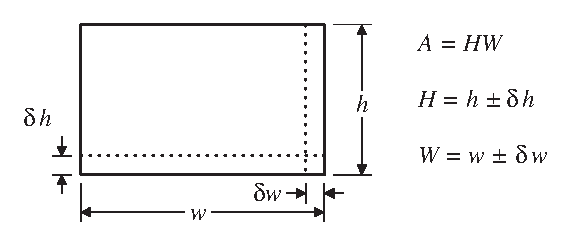
\includegraphics{figa1.eps}}}}
\end{center}
%   \centerbmp{3.72in}{1.43in}{errarea.bmp}
% \vspace{1.5in}
%  \hspace{2in}
% \special{bmp:errarea.bmp x=3.44in y=1.5in}
%\special{eps:figa1.eps x=3.44in y=1.5in}
%\special{wmf:figa1.wmf} % x=3.44in y=1.5in}
 \caption{Calculation of the area of a rectangle.  \label{fig:rect}}
\end{figure}
Clearly the best estimate for the area is $A=3.97\times2.73=10.8381\;{\rm cm^2}$.
A high estimate can be obtained by using the largest possible $W=3.97+.03=4.00$~cm
and the largest possible  $H=2.73+.03=2.76$~cm: 
$A_{\mbox{max}}=4.00\times2.76=11.04\;{\rm cm^2}$. Similarly,
a low estimate can be obtained by using the smallest possible $W=3.97-.03=3.94$~cm
and the smallest possible  $H=2.73-.03=2.70$~cm: 
$A_{\mbox{min}}=3.94\times2.70=10.638\;{\rm cm^2}$. So it seems that
$A$ must be in the range $10.638\mbox{--}11.04\;{\rm cm^2}$, which we can summarize as
$A=10.8381\pm 0.201 = 10.8\pm 0.2\;{\rm cm^2}$, where $\delta A$ was estimated
as $(A_{\mbox{max}}-A_{\mbox{min}})/2$.  We call this process of finding the
error in a calculated quantity by repeated calculation using extreme values
the ``high-low game".  It represents the crudest form of error propagation.
Some deficiencies are: (1) In a more complicated calculation, it will not clear what combination
of high and low inputs produces the extremes, so all combinations must be tested.
(2) Since the resulting error comes as the end result of a complex process, you cannot
answer important questions like: ``Which measured quantity most contributes
to the error?" or ``How much do I need to reduce the errors in the measurements to
achieve a particular accuracy in the result?".  (3) The method does not take into
account the unlikeliness of the measured quantities conspiring to achieve exactly the
right combination of extreme values to produce the extreme calculated result.

We can simplify the calculations (and solve problems (1) and (2)) by doing
the algebra for a general case.
We write the formula for the area $A$ and its uncertainty $\delta A$
as follows:
\begin{eqnarray*}
%A & = & (\ell \pm \delta \ell) \: (w \pm \delta w) \\
%  & = & \ell w  \pm \ell \: \delta w  \pm w \: \delta \ell + \delta \ell \:
%        \delta w
A \pm \delta A& = & (h \pm \delta h) \: (w \pm \delta w) \\
  & = & h w  \pm h \: \delta w  \pm w \: \delta h + \delta h \:
        \delta w
\end{eqnarray*}
An examination of the diagram should persuade you that the last
term, which is represented by the small square in the lower right-hand
corner, is much smaller than the second and third terms, represented
by the two small rectangles.  Hence to a good approximation the
best estimate for the area and its
uncertainty are given by
\begin{eqnarray*}
%\delta A = \ell \: \delta w + w \: \delta \ell
A &=& hw \\
\delta A &=& h \: \delta w + w \: \delta h
\end{eqnarray*}
where we have used the signs producing the maximum
value, so
that the uncertainties added rather than partially canceling.  Because
we have not allowed for partial cancelation, we call the resulting
error estimates ``worst-case errors".

 Note that we can also write this equation as
\begin{eqnarray*}
%\delta A & = & {{\ell w} \over {w}} \: \delta w + {{\ell w} \over {\ell}} \:
%               \delta \ell \qquad \mbox{or} \\
%\delta A & = & A \: \left({{\delta w} \over {w}} + {{\delta \ell} \over {\ell}}
%               \right)
\delta A & = & {{h w} \over {w}} \: \delta w + {{h w} \over {h}} \:
               \delta h \qquad \mbox{or} \\
\delta A & = & A \: \left({{\delta w} \over {w}} + {{\delta h} \over {h}}
               \right) \qquad \mbox{or} \\
{\delta A \over A}& = & {{\delta w} \over {w}} + {{\delta h} \over {h}}
\end{eqnarray*}
Since $\delta A/A$ is the relative error in $A$ this last equation says
that the relative error in $A$ is the sum of the relative errors in $w$ and $h$.

While we do not reproduce the proof here, a
more advanced statistical treatment shows that the likelihood of
partial cancelation of multiple errors (problem (3) above) can
best be addressed by using the following error estimate: 
\[
%\delta A = A \: \sqrt{ \left({{\delta w} \over {w}} \right)^{2} + \left(
%           {{\delta \ell} \over {\ell}} \right)^{2} }
\delta A = A \: \sqrt{ \left({{\delta w} \over {w}} \right)^{2} + \left(
           {{\delta h} \over {h}} \right)^{2} }
\]
In words, this equation states that the percentage error in the
area is the square root of the sum of the squares of the
percentage errors in $h$ and $w$.  %$\ell$ and $w$.

Table~\ref{table1} gives the result of this
calculation for several commonly used operations.  Note that Eq.~A.2 in
that table is identical to the result we found above for the
uncertainty in the area.
It would be a useful exercise for you to confirm all of these results.

\begin{table}[ht]
\begin{center}
\caption{Formulae to calculate the error resulting from various operations.
   \label{table1}}
\vspace{12pt}
\begin{tabular}{|llll|}
\hline
 & & &   \\
{\bf Operation} & {\bf Form} & {\bf Estimated Error} & \\
 & & &   \\
\parbox{1.1in}{Addition\\
\hspace*{1ex} or Subtraction} & \parbox{.6in}{$z = x+y$ \\ $z=x-y$} &
   $\delta z = \sqrt{  (\delta x)^{2} \mathstrut+ (\delta y)^{2} } $ & (A.1) \\
 & & & \\
\parbox{1.1in}{Multiplication \\
\hspace*{1ex} or Division}& \parbox{.6in}{$z = xy$ \\ $z=x/y$} &
${\displaystyle\delta z=|z| \: \sqrt{ 
\left( { \delta x  \over x} \right)^2+
\left( { \delta y  \over y} \right)^2}}$
   & (A.2) \\
 & & &   \\
Powers & \parbox{.8in}{
$z = x^{m}\;y^{n}$\\ ${z} = x^{m}/y^{n}$} &
   $ {\displaystyle\delta z = |z| \: \sqrt{ \left (m \: {{\delta x}
\over
{x}}\right)^{2} + \left(n \: {{\delta y} \over {y}}\right)^{2} }}$ & (A.3)
\\ & & & \\
Function & 
$z = f(x)$ &
   $ {\displaystyle\delta z = \left|f'(x)\right|\; \delta x}$ & (A.4)
\\ & & & \\
\hline
\end{tabular}
\label{errorprop}
\end{center}
\end{table}

{\bf Example: }
Take a moment to look over the equations in Table~\ref{table1}.  To
illustrate how these formulas are used, we will use the distance ($S$)
and time ($t$) measurements given in Table~\ref{table2} below to find
the average velocity and the error in velocity in the interval from
$t_1$ to $t_3$.  The average velocity $v$ is given by
\[
v = {\Delta S \over {\Delta t}} = {{S_{3} - S_{1}} \over {t_{3} -
t_{1}}} .
\]

\begin{table}[ht]
\begin{center}
\begin{tabular}{|cll|}
\hline
point \# & $S$ (cm) & $t$ (sec) \\ \hline
1 & $0.00 \pm 0.05$ & $0.000 \pm 0.002$ \\
2 & $0.25$ & $0.016$ \\
3 & $0.71$ & $0.032$
\\ \hline
\end{tabular}
\end{center}
\caption{Sample distance and time data.  \label{table2}}
\end{table}

There are three steps in this calculation:  We find the error in the
numerator, then the error in the denominator, and finally, we find
the error in the velocity.

Consider the numerator.  Note that both $S_3$ and $S_1$ have
uncertainties.  Hence to find the uncertainty in
$ \Delta S = S_{3} - S_{1} = 0.71$ cm, we apply Eq.~A.1 to obtain an
uncertainty of
\[
\delta (\Delta S) = \sqrt{ (0.05)^{2} + (0.05)^{2} } = 0.07 \;
\mbox{cm} \]
To find the error in the denominator, we use the same equation.
Here $\Delta t = t_{3} - t_{1} = 0.032 \; \rm{s}$.  The uncertainty
in $\Delta t$ is
\[
\delta (\Delta t) = \sqrt{ (0.002)^{2} + (0.002)^{2} } = 0.003 \;
\mbox{s}
\]
The average velocity $v$ is
$v = 0.71/.032 \; \mbox{cm/s} = 22 \; \mbox{cm/s}$
And since we have the uncertainties in both
\[
\Delta S = 0.71 \pm 0.07 \; \rm{cm}
\]
and
\[
 \Delta t = 0.032 \pm 0.003 \; \rm{sec},
\]
we can find the error in $v = \Delta S / \Delta t$, using Eq.~A.2:
\[
\delta v = 22 \: \sqrt{ \left({{0.07} \over {0.71}}\right)^{2} +
           \left({{0.003} \over {0.032}}\right)^{2} } \; \mbox{cm/s} \:
         \approx 3 \; \mbox{cm/s}
\]
 Therefore the average velocity should be reported as $22 \pm 3$ cm/s.
Note that it would make no sense to report this result as $ 22.1875\pm 3$ cm/s;
the fractional part of the speed is of no significance if the uncertainty  is 3 cm/s.
Similarly, given the crude nature of our estimates of error, one or at most
two significant digits in the uncertainty should be reported.  
Note a fast way to lose lots of points: $ 22.1875\pm 2.99308$ --- no units and 
too many significant digits in both the number and the error.

Since the numerical value of  constants (such as
$\pi$ or $\ln(2)$) are known to very high precision, they should
be treated as error-free in calculations.  


\subsubsection*{Optional Derivation}
     In the above example the uncertainty was easy to calculate
directly.  In general, however, such will not be the case.
Therefore we will introduce a more general method of finding the
error in a calculated quantity.  The derivation involves using
calculus, and may prove difficult for beginning students to
follow in detail.  But don't give up --- what is hard for you to
understand now will seem much easier in a semester or so, when
you are farther along in your mathematics.  Until then, you can
simply use the results given in Table~\ref{table1} above.

     Consider a calculated quantity $z$ that is a function of the
measured quantities $x$ and $y$; that is, $z = z(x,y)$.  How can we
calculate $\delta z$, the uncertainty in $z$, from our measurements
$(x \pm \delta x, y \pm \delta y)$,
assuming the uncertainties $\delta x$ and $\delta y$ are random and
independent.  We begin by calculating the differential of $z$:
\[
dz = {{\partial z} \over {\partial x}} \, dx +
            {{\partial z} \over {\partial y}} \, dy
\]
(The symbol $\partial$ indicates a partial derivative---see your
calculus text if you have not yet encountered this concept.) If
the uncertainties $\delta x$ and $\delta y$ are not too large, we can
replace the differentials by the corresponding uncertainties and
write
\[
\delta z \approx \left|{{\partial z} \over {\partial x}} \, \delta x \right| +
            \left| {{\partial z} \over {\partial y}} \, \delta y \right|
\]
where we have used absolute value signs so that
uncertainties with different signs will not cancel.  This
expression gives the worst-case estimate for the uncertainty
in $z$.  A more advanced statistical treatment (allowing for partial cancelation) shows
that this expression is a bit too pessimistic, and that a better
estimate is given by taking the square root of the sum of the
squares of all the terms:
\[
\delta z \approx \sqrt{ \left({{\partial z} \over {\partial x}} \, \delta x
                 \right)^{2} + \left( {{\partial z} \over {\partial y}} \,
                 \delta y \right)^{2} }
\]
Once can derive all of the formulas in Table~\ref{table1} and Appendix E, as well as
the equations for more complex cases, using this technique.  See
Taylor's book, previously cited, for a more detailed treatment.

\subsection*{Uncertainties in Functional Parameters}
     We have seen how to estimate errors in measured quantities,
and in quantities calculated from those measured quantities.
However, often our goal is to find functional
relationships between measured quantities.  For example, suppose we
have a set of measurements of velocity and time that lie roughly along
a straight line.  The functional relationship between them is
therefore linear and can be written
\[
v = A + Bt
\]
where $v$ is velocity, $t$ is time, and $A$ and $B$ are constants
(here, the intercept and slope of the line).  Since the points will
not all lie exactly on the straight line, there will be a range of
possible slopes and intercepts that will all describe the data
reasonably well.  Under such circumstances, how
could we find the uncertainties in the parameters, $A$ and $B$, from
the uncertainties in $v$ and $t$?

     We will discuss this question more fully in the next three
appendices, and as usual, refer the reader to Taylor's book for a more
complete discussion.

%  The basic test that should be used in
%estimating parameter error is how much can the parameter be
%changed without changing the ability of the relationship to give
%an acceptable description of the data.  Clearly the error in
%these parameters depends on our definition of acceptable (and has
%no meaning if the fit was unacceptable to start with).  The
%errors also depend on the method of analysis and whether the
%error in the measurements have been estimated correctly.  We will
%let a computer estimate the parameter errors for more
%sophisticated functional relationships (see sections on Data Analysis,
%p.~\pageref{datanal}, and Computer Assisted Curve Fitting,
%p.~\pageref{compassis}).



\renewcommand{\newname}{APPENDIX B---Tables and Graphs}
%APPENDIX B--TABLES AND GRAPHS
\newapp
%\section*{Data Handling}
%\addcontentsline{toc}{subsection}{Data Handling}
%\label{datahandle}
\section*{Tables}
     Experimental data are usually recorded in tabular
form (see Table~\ref{tableb2}).  The table should have labeled columns for the
both the independent and dependent variables.  Each column label should show
the units for that quantity.  A representative estimate of the
error should be made and recorded for the first entry in a column
and any other place that the value of the error changes
significantly.  (In this example the uncertainty in distance, $\delta S$,
and the uncertainty in time, $\delta t$, are the same for each
of the three data points; it is not uncommon to have varying uncertainties---
requiring a column just for uncertainty.  In addition if you are using a spreadsheet
to record values, enter numbers only, without the $\pm$.) Room for extra columns should be left if
quantities are going to be calculated from the direct
measurements.  A sample calculation should also be shown at the
bottom of the table for those quantities which are calculated.
\begin{table}[h]
\begin{center}
\begin{tabular}{|cll|}
\hline
point \# & $S$ (cm) & $t$ (sec) \\ \hline
1 & $0.00 \pm 0.05$ & $0.000 \pm 0.002$ \\
2 & $0.25$ & $0.016$ \\
3 & $0.71$ & $0.032$
\\ \hline
\end{tabular}
\end{center}
\caption{Sample distance and time data.  \label{tableb2}}
\end{table}
\begin{figure}    %linear graph of distance vs time
\begin{center}
{\resizebox{3.5in}{!}{\rotatebox{-90}{\includegraphics{appb_TB1.ps}}}}\hfill
\raisebox{-2.25in}{\resizebox{2.25in}{!}{{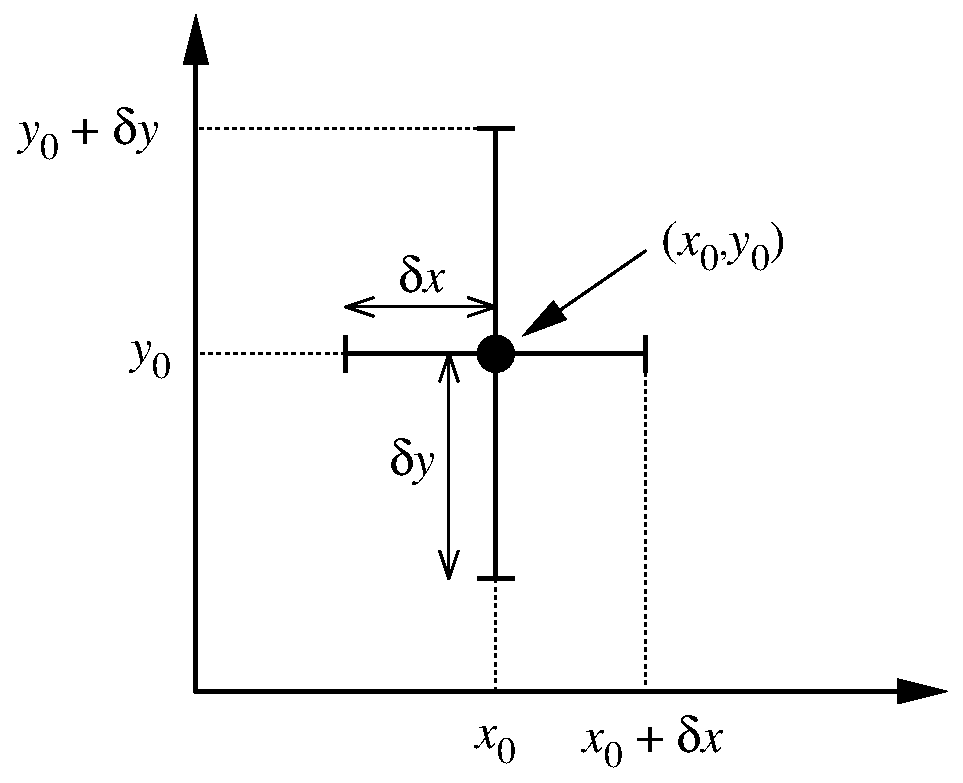
\includegraphics{errbarsB.eps}}}}
\end{center}
%\vspace{4in}
%\centerbmp{6.94in}{9in}{pressure.bmp}
%\special{ps:pressure.ps}
\caption{Plot of the data presented in Table~\protect\ref{tableb2} and
a typical graphed data point.  \label{fig:b1}}
\end{figure}

\section*{Graphs}
     Since it is much easier to recognize a pattern from a graph
(picture) than from a table, we will use graphs extensively in
this laboratory.  (The next Appendix, Graphical Analysis, will show you how to
recognize functional relationships from graphs.)

     Whenever possible, make an initial graph to monitor the experiment {\em as
you are collecting the data}.  As you record each measurement in a table,  plot it
on the graph.  After several points have been graphed, a pattern
(or shape) becomes apparent.  This pattern can then serve as a
general guide to tell whether subsequent measurements fit the
pattern.  Although we may not know the exact pattern the data
will follow, large deviations from any pattern can be easily
identified, thus catching problems in time to correct them.
This initial graph will also serve as the starting point for data
analysis.

     A final graph should always be included in your lab
write-up.  This graph should be a refined and more complete
version of your initial graph.  See Appendix C on Graphical Analysis for
several examples of properly prepared final graphs.  To insure that the
graphs give a clear picture of what is being represented, we ask
you to follow this set of rules:
%\begin{figure}[hbt]
%\begin{center}
%{\resizebox{3in}{!}{{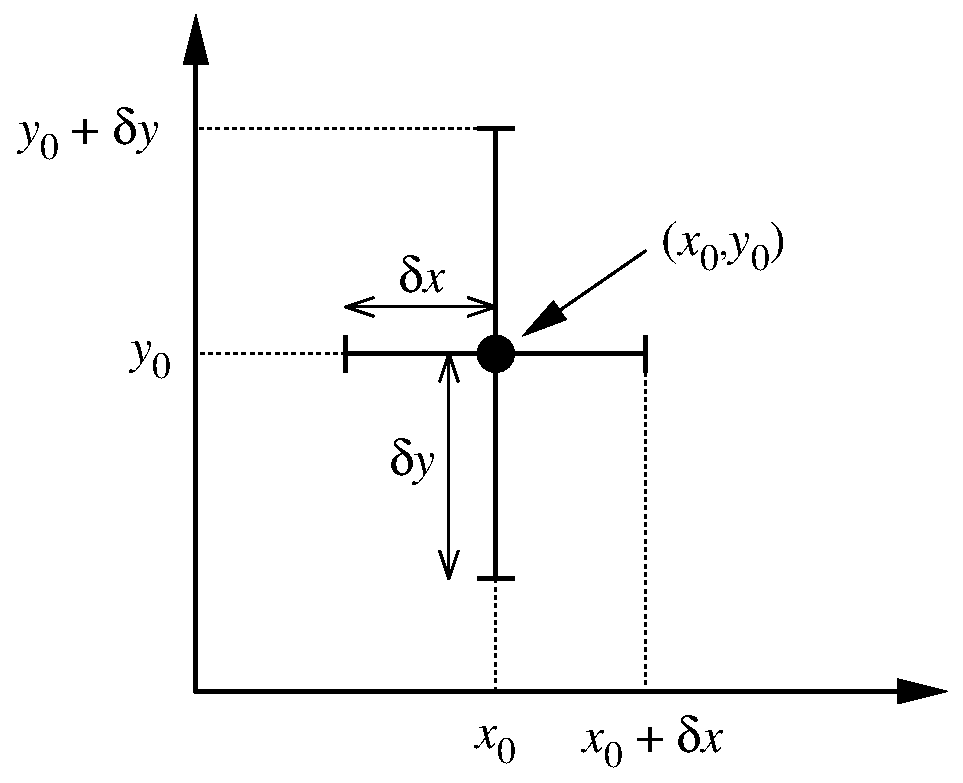
\includegraphics{errbarsB.eps}}}}
%\end{center}
%   \centerbmp{3.72in}{2.2in}{errbars.bmp}
% \caption{A typical graphed data point.  \label{fig:b1}}
%\end{figure}
\begin{enumerate}
\item Put a title on each graph in a place that will not
           obscure the data.
\item Label each axis with the name of the quantity and its
           units.
\item Select the graph scale such that the data spans most of
           a full page of graph paper --- {\em DO NOT} plot all of your
           data in one small section of the page!
\item On your final graph indicate the error in each graphed
           data point by using error bar symbols.
           An example of a typical graphed data point ($x_{\circ},y_{\circ}$)
           with error bars is shown in Fig.~\ref{fig:b1}.
           You need not show error bars that are smaller than the
           dot size.  However, note the fact that the errors are
           smaller than dot size below the graph's title.
\item {\bf Optional:}  With a pencil, lightly sketch a {\em smooth}
           curve through the data (do not play
           ``connect the dots'').  If this is an initial graph, the
           curve should represent your ``eyeball" approximation
           of the pattern.  For the final graph the smooth curve
           should be based upon your graphical or computer data
           analysis (as explained in the next two sections).
\end{enumerate}


\renewcommand{\newname}{APPENDIX C---Graphical Analysis and Functional Forms}
%APPENDIX C--GRAPHICAL ANALYSIS AND FUNCTIONAL FORMS--191
\newapp
\label{datahandle}
{\bf PLEASE NOTE:}  In this appendix and the following one,
 we discuss what is sometimes
called ``curve fitting''---seeing how well particular equations
describe a set of experimental data.  {\em The treatment of curve
fitting
in this appendix is brief, and is not intended to be complete!}
For a more complete treatment we strongly recommend the book {\em An
Introduction to Error Analysis} by John R.~Taylor.

\section*{Introduction}

     In any experiment, only a limited number of measurements of
the experimental observables are made.  In order to see if our
measurements conform to a theoretical prediction, or to calculate
the values of experimental observables for situations that we
have not measured, we often need to establish a mathematical
relationship between experimental observables.  This process is the
task of curve-fitting.

    If two variables are related, then when one is changed there will
always be a corresponding change in the other.  Suppose variable $x$
is controlled in the experiment, and we are observing how the value of
variable $y$ is affected.  We call $x$  the {\em independent} variable
and $y$  the {\em dependent} variable.

We suppose there is a mathematical function $y(x)$
(in words, $y(x)$ is read ``$y$ as a function of $x$"), that
approximately
describes the way the two variables are related.  One simple example of
such a function is the equation of a straight line:
\[
y(x) = A + Bx .
\]
The constants $A$ and $B$ are called the {\em parameters} of the
function---in this case, the $y$-intercept and the slope of the line.
Briefly, then, our job in curve fitting is to
find the equation $y(x)$ that best describes the
experimentally measured quantities $(x, y)$,   and
establish what specific values of the parameters work best for our
data.

     We will introduce you to two methods of curve fitting that
are useful for finding functional relationships; they are
\begin{itemize}
	\item {\em graphical analysis}: using semi-log and log-log
graphs to ``linearize'' our data; and
%	
	\item {\em the method of least squares}.  For this method,
	we will use a computer program, Linfit, that is described in
	Appendix D.
\end{itemize}	
For either
of these methods the initial steps in data analysis are the same:

\begin{enumerate}
\item Choose one of the experimental observables to be the
           independent ($x$) variable.  In general, choose either
           the quantity which is most easily controlled
           experimentally or the quantity which has the smallest
           error.  The other variable ($y$) is called the dependent
           variable.
	
\item Make a careful graph of the data --- ``$y$ vs. $x$" --- in your lab notebook, as
	discussed in the Appendix on Tables and Graphs.  Plot
	$y$ (the {\em dependent} variable) on the vertical axis and
$x$ (the
	{\em independent} variable) on the horizontal axis.  Include error
	bars to indicate the uncertainties of the variables at each data
	point.  (see Appendix B).

\item With a pencil, lightly sketch a smooth curve through the data
and try to guess what function would match the curve.  Theory often suggests
an appropriate guess---for example, radioactive decay is
usually consistent with an exponential function.  Other examples are
given below.

\item Test your guess, either by computer curve-fitting or by graphing the
    data in such a way that a straight line should result if your guess is
    correct.  More explanation of this step is given below.

\item If your analysis is satisfactory, you will have both the function and
    its parameters for approximating your data.
	
\end{enumerate}
\label{datanal}


\section*{Graphical Analysis: Lines}

Suppose we have done an experiment and made a careful graph of the data.  If
the data lie on a straight line, our task is comparatively easy.  Often,
however, the data will describe a curve.  We want to find out what function
describes that curve.  Is it a quadratic?  a cubic?  part of a sine
curve?  Or some other function?  How can we tell?

For two important classes of functions, exponential functions and power laws, it
turns out that ``semi-log'' graphs ($\log y$ vs. $x$) or ``log-log''
graphs ($\log
y$ vs. $\log x$) can transform the data to a straight line, which is
always
easy to recognize.  If this method works, then the parameters of the
function can then be estimated from the line, as we shall see below.

Only rarely, of course, will our data points lie exactly on a line.  A line is
generally considered to be an acceptable description
if it passes through the error bars of roughly 2/3 of the data points.  (See
Taylor for a detailed explanation.)


\paragraph*{1. Linear Function}
     We begin by considering the  linear function (or straight line), which
as we have already seen, can be written as
\begin{equation}
y = A + Bx  \label{eq:c1}
\end{equation}
The parameters $A$ and $B$ specify the particular straight line
that describes a given set of data.  Frequently
the experimental result that we seek is one of these parameters.

A graph of $y$ versus $x$, with error bars
on all the points, will show whether a straight line is acceptable.  Most
likely, there will be a range of acceptable lines, as illustrated
in the Figure below.
From them you can estimate the parameters $A$ and $B$ with their uncertainties.

\begin{figure}[hbt]    %Appendix C, Fig 1
%\centerbmp{3in}{2.5in}{gpherror.bmp}
\begin{center}
{\resizebox{3in}{!}{{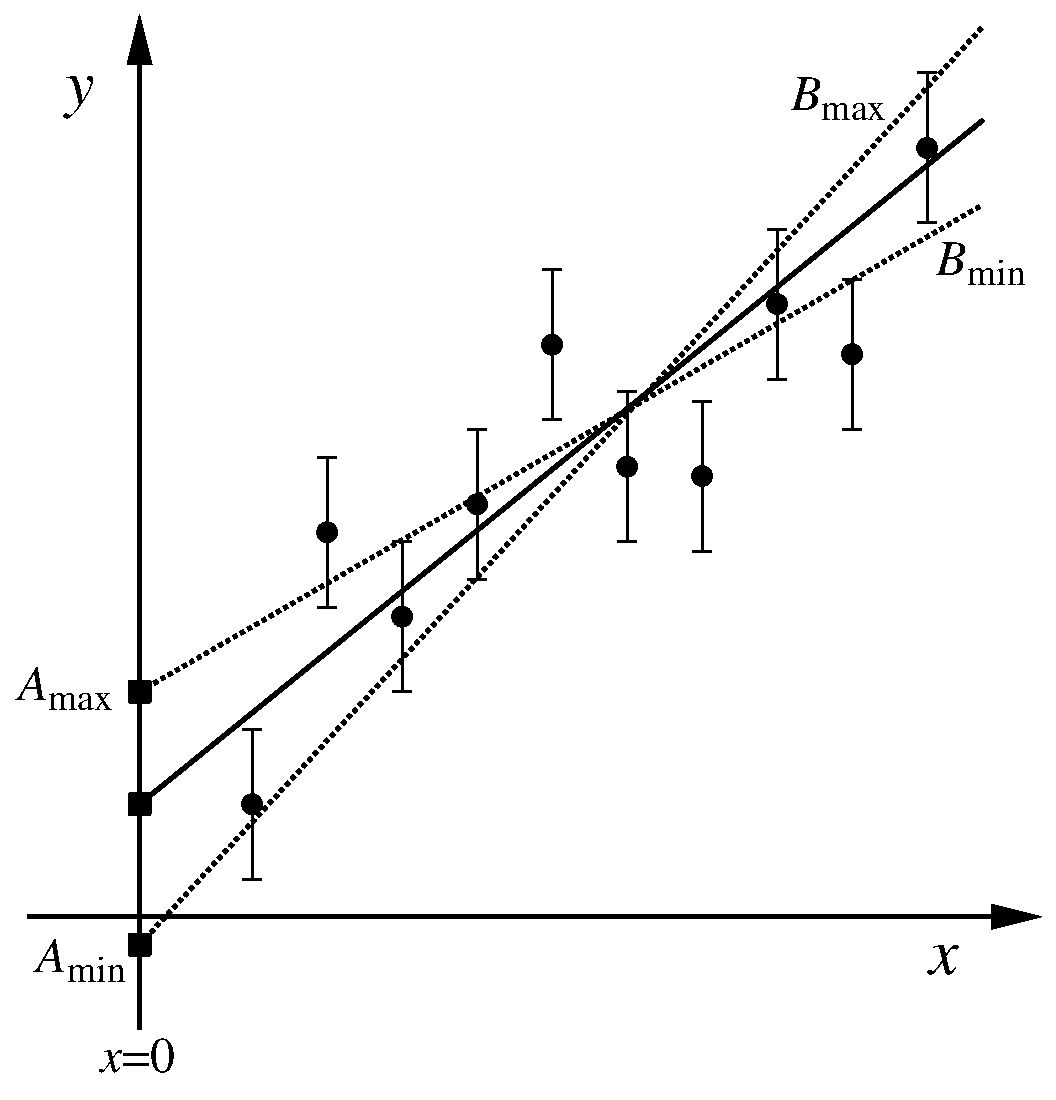
\includegraphics{gpherrB.eps}}}}
\end{center}
\caption{Finding the uncertainty in slope by hand (approximation)  \label{fig:slope}}
\end{figure}

 Our goal is to determine the parameters $A$ and $B$ from the
graph.  If the experimental data fall more or less on a straight
line (that is, it they satisfy the ``two-thirds criterion" for
a linear relationship), then we can obtain estimates for the
parameters $A$ and $B$ from the algebraic properties of a linear
function and the smooth curve (straight line) drawn through the
graphed data points.  For a linear relationship we note that any
two points $(x_{1}, y_{1})$ and $(x_{2}, y_{2})$ {\em on the line} can be used
to find an estimate for the slope of the line, $B$, since
\begin{eqnarray*}
y_{1} & = & A + Bx_{1} \\
y_{2} & = & A + Bx_{2}
\end{eqnarray*}
so that
\[
y_{2} - y_{1} = B(x_{2} - x_{1})
\]
 or
\[
B = {{y_{2} - y_{1}} \over {x_{2} - x_{1}}}
\]
Note that the units of $B$ are the units of $y/x$.

{\bf IMPORTANT: Do not} use two data points to find the slope!!
Rather use two well-separated points {\em on the line you have sketched}, which
represents information from {\em all} of the data points.

To estimate the $y$-intercept $A$, use one of the
following two methods: \begin{enumerate}
\item If the vertical line $x=0$ is physically on your graph,
then you can probably find where your sketched line intersects it.
The parameter $A$ is the
           value of $y$ where your sketched line
reaches $x=0$ (the ``$y$-intercept").
\item If the $y$-intercept is not on your graph (and very
           often it will not be), we simply note that the values
           for any point on the {\em line} can be used to solve for $A$,
           once we know the slope $B$, since $A = y_{i} - Bx_{i}$.
This method will usually be less accurate than the first.
\end{enumerate}

{\bf Example: }
     As an example let's try to see whether the temperature ($T$)
of a certain metal rod is linearly related to distance along the
rod ($d$).  The experimental observations are given in Table~\ref{table:temp}
and plotted in \ref{fig:temp}.
\begin{table}[h]
\begin{center}
\begin{tabular}{|ll|}
\hline
$d$ (cm) &\hspace{5pt} $T$ ($^{\circ}$C)  \\ \hline
 1 $\pm$ 0.01& \hspace{5pt} 16 $\pm$ 4  \\
2& \hspace{5pt} 18  \\
3& \hspace{5pt} 35  \\
4& \hspace{5pt} 44  \\
5& \hspace{5pt} 58  \\
6& \hspace{5pt} 62  \\
7& \hspace{5pt} 64  \\
8& \hspace{5pt} 70  \\  \hline
\end{tabular}
\end{center}
\caption{Sample data of temperature as a function of distance along a metal
         rod.  \label{table:temp}}
\end{table}


\begin{figure}[!hbt]     %Appendix C, Fig 2: temp vs distance
\begin{center}
{\resizebox{5in}{!}{\rotatebox{-90}{\includegraphics{temp_disB.ps}}}}
\end{center}
%\vspace{4in}
%\centerbmp{6.92in}{9in}{tempvsd.bmp}
%\special{ps:temp_dis.ps}
\caption{Graph of the data presented in Table~\protect\ref{table:temp}.
          \label{fig:temp}}
\end{figure}

It is straightforward to measure the slope $B$, as shown above.  The
uncertainty in the slope can be
estimated from the ``best" line (as judged by eye), and from
upper and lower outer limits of possible slopes that might
work, (for example, the dotted lines in Fig.~\ref{fig:slope} above).
As an exercise, try to find $A$, $B$ and their
uncertainties; you should find something like
\begin{equation}
A  =  8 \pm 4 \;^{\circ}\mbox{C}, \ \ \ \
B   =  8 \pm 1 \;^{\circ}\mbox{C/cm}
\end{equation}

\section*{Graphical Analysis: Curves}


    It is fairly easy to determine whether a set of data lies on
a straight line.  But what if it doesn't --- what if the smooth line
drawn through a set of data in fact curves?  How can we
decide whether that curve represents a quadratic, or a cubic, or
some other function?  The next two sections will show
how two fairly common functional forms, power laws and
exponentials, can be transformed so that they look like straight
lines, and hence can be easily identified and analyzed.  The
same sort of transformation process applies to many functional forms.

    These two sections will be primarily concerned with graphical
analysis, but we can also use the method of least squares to find the
``best" values for the function parameters and their
uncertainties---see Appendix D.

\paragraph*{2.  Exponential Function}
\label{exprel}
An exponential function takes the form
\begin{equation}
y = A\, e^{Bx}     \label{eq:c4}
\end{equation}
where $e$ is the base of natural logarithms.

This function is not linear, and hence will
show some curvature on a linear graph.
%\subsection*{Exponential Graphical Analysis}
     To  analyze exponential relationships graphically, we
begin by taking the logarithm of both sides of  the above
exponential equation, Eq.~\ref{eq:c4}.
%\begin{equation}
%y = A\, e^{Bx}  \label{eq:c4a}
%\end{equation}
Recall that for natural logarithms,
\[
\ln e^{t}  = t
\]
and
\[
\ln AB = \ln A + \ln B .
\]
So taking the the natural logarithm of both sides of
Eq.~\ref{eq:c4}, we obtain
\begin{equation}
\ln y = \ln(A \, e^{Bx}) = \ln A + \ln \, e^{Bx}
   = \ln A + Bx   \label{eq:c5}
\end{equation}
If we now define $Y \equiv \ln y$ and $C \equiv \ln A$, this
equation becomes \[
Y = C + Bx
\]
which is the equation of a straight line with slope $B$ and
intercept $C$!  Thus if we plot $Y$ versus $x$ (that is,
$\ln y$ versus $x$) and obtain a straight line, we may infer that our
data can be described by an exponential function.  A graph of
$\ln y$ versus $x$ is often called a semi-log graph.

Note that we have used natural (base $e$) logarithms in this section
instead common (base 10) logarithms.  Either will linearize an exponential
relationship
(although natural logarithms are widely used in science and engineering).
  In either case,
it is easy to find the logarithms, either with a calculator or a
spreadsheet (such as Excel\footnote{
In Excel {\tt log10()}=$\log_{10}()$ and {\tt ln()}=$\log_e()$.
 {\tt log()} by itself is ambiguous: in Excel it is $\log_{10}()$
but in most computer languages it is $\log_e()$.}
%
 or the similar spreadsheet module in
Linfit).

Suppose, then, that our data can be described by a straight line
on a semi-log graph.  We can find the slope $B$ and intercept $C$
from this second graph, exactly as described above.
Thus, the slope can be calculated by picking two points
on the line of the graph of $\ln y$ vs.\ $x$ and calculating
\begin{equation}
B = {{Y_{2} - Y_{1}} \over {x_{2} - x_{1}}} = {{\ln y_{2} - \ln y_{1}}
           \over {x_{2} - x_{1}}} = 
{\ln\left(y_{2}/y_{1}\right) \over x_{2} - x_{1}}  \label{eq:cnew}
\end{equation}
Note that the units of $B$ are the units of $1/x$.

The intercept $C$ can likewise be easily found, and once we have it,
we can find the parameter $A$ by observing that

%\begin{enumerate}
%\item A graph of the calculated values of $\ln y$ vs.\ $x$ on
%           linear graph paper (see Fig.~\ref{fig:c3b} and Fig.~\ref{fig:c3b1}).
%\item A graph of $y$ vs.\ $x$ on semi-log paper which has the
%           $y$-axis stretched in such a way as to do the linear
%           transformation for us (see Fig.~\ref{fig:c3c}).
%\end{enumerate}
%
\[
C = \ln A  \qquad \mbox{or} \qquad  A = e^{C}
\]
Note that the units of $A$ are the units of $y$.

Thus we have found the parameters $A$ and $B$ that describe our
exponential function.

%In addition an
%exponential has a constant doubling interval and this property
%can be used to distinguish it from a power relationship.  To
%calculate the doubling interval of a curve, pick some small $y$
%value (say $y_{1}$) and note the $x$ coordinate (say $x_{1}$).  Then find the
%$x$ coordinates where $y = 2y_{1}$ and $4y_{1}$ (call them $x_{2}$ and $x_{4}$).
%If
%\[
%x_{2} - x_{1} \approx x_{4} - x_{2}
%\]
%then the doubling interval is approximately constant.  For
%example, find the doubling interval for the data for altitude, $H$,
%versus  given in the Table~\ref{table:c3a} and
%plotted in Fig.~\ref{fig:c3a} and Fig.~\ref{fig:c3a1}.

{\bf Example: }
As an example, consider the data for atmospheric pressure, $P$,
versus altitude, $H$, given in the following table.
% atmospheric pressure, $P$, given in the Table~\ref{table:c3a} and
%plotted in Fig.~\ref{fig:c3a} and Fig.~\ref{fig:c3a1

\begin{table}[h]
\begin{center}
\begin{tabular}{|rlrcc|}
\hline
$H$ (km) & $P$ (bars) & $\ln P$ & $\ln (P + \delta P)$ & $\ln (P - \delta P)$ \\
 \hline
0.0 \hspace{6pt}  & 1.00 $\pm$ 0.03 & 0.00    & +0.03     &  $-$0.03\\
2.0 \hspace{6pt}  & 0.75            & $-$0.29 & $-$0.25   &  $-$0.22 \\
4.0 \hspace{6pt}  &     0.60        & $-$0.51 &   $-$0.46 &  $-$0.56 \\
5.0 \hspace{6pt}  &     0.48        & $-$0.73 &   $-$0.67 &  $-$0.80 \\
7.5 \hspace{6pt}  &   0.37          & $-$0.99 &   $-$0.92 &  $-$1.08  \\
10.0 \hspace{6pt} &   0.27          & $-$1.31 &   $-$1.20 &  $-$1.43 \\
15.0 \hspace{6pt} &     0.14        & $-$1.97 &   $-$1.77 &  $-$2.21 \\
20.0 \hspace{6pt} &     0.07        & $-$2.66 &   $-$2.30 &  $-$3.22 \\
\hline
\end{tabular}
\end{center}
\caption{Sample data of pressure vs.\ height in the atmosphere.
     \label{table:pressure}}
\end{table}

Please inspect carefully the table, and the two graphs on the following
page.  The first graph (a straightforward plot of $P$ vs.\ $H$)
shows a curve.  The second is a semi-log graph (that
is, a graph of $\ln(P)$ vs.\ $H$) that shows a straight line.  
(Note that the log scale
changes the appearance of the error bars: they are not symmetrical
and the bar size has changed from the ``normal" plot.\footnote{That final error bar
ranges from $\ln(0.04)=-3.22$ to $\ln(0.10)=-2.30$ with ``anchor" at $\ln(0.07)=-2.66$.})  

Since this second
graph is linear, we may infer that these data are consistent with an
exponential function.  As an exercise, see if you can determine the
parameters $A$ and $B$ in Eq.~\ref{eq:c4}, above by making your own
semi-log graph and finding the slope and intercept.

\newpage

\begin{figure}[!hbt]    %linear graph of pressure vs altitude
\begin{center}
{\resizebox{5in}{!}{\rotatebox{-90}{\includegraphics{pressureB.ps}}}}
\end{center}
%\vspace{4in}
%\centerbmp{6.94in}{9in}{pressure.bmp}
%\special{ps:pressure.ps}
\caption{Graph of the data presented in Table~\protect\ref{table:pressure}.
          \label{fig:pressure}}
\end{figure}

\begin{figure}[!hbt]   %semi-log graph of pressure vs altitude
\begin{center}
{\resizebox{5in}{!}{\rotatebox{-90}{\includegraphics{pressure_logB.ps}}}}
\end{center}
%\vspace{4in}
%\special{ps:pressure_log.ps}
\caption{Semi-log graph of the data presented in Table~\protect\ref{table:pressure}.
          \label{fig:pressure_log}}
\end{figure}



\paragraph*{3. Power Law}


    By a power law we mean an equation of the form
\begin{equation}
y = Ax^{B}  \label{eq:c3}
\end{equation}
If $B = 2$, for example, we have a quadratic.
In general, a power law equation shows curvature.

     Once again we begin by taking the natural logarithm of both sides of the
power-law equation. 
%\[
%y = Ax^{B}.
%\]
As we shall see, this step will ``linearize'' the equation --- 
the technique is similar to the one we used for
exponentials.  Taking the logarithm of both sides of the equation, we
obtain
\[
\ln y = \ln (Ax^{B}).
\]
And since
\begin{eqnarray*}
\ln (Ax^{B}) & = & \ln A + \ln (x^{B}) \\
              & = & \ln A + B \: \ln x
\end{eqnarray*}
we obtain the result
\[
\ln y = \ln A + B \: \ln x .
\]
If we define two new variables $Y \equiv \ln y$ and $X \equiv \ln
x$ and
a new constant $C \equiv \ln A$ then we obtain the transformed
equation
\[
Y = C + BX
\]
which is the equation of a straight line!

  Therefore, to find out if our data are consistent with a power law,
we make a graph of
$Y$ versus $X$ (that is, $\ln y$ versus $\ln x$).  Such a graph
is often called a ``log-log'' graph.  If our data lie along a straight
line on the log-log plot, then we can say that those data are consistent
with a power law.

We can find the slope $B$ and
the intercept $C= \ln A$ as before.  In this case, the slope $B$ is
given by
\[
B = {{Y_{2} - Y_{1}} \over {X_{2} - X_{1}}} =
    {{\ln y_{2} - \ln y_{1}} \over {\ln x_{2} - \ln x_{1}}} =
{\ln\left(y_2/y_1\right) \over \ln\left(x_2/x_1\right) }
\]
Note that this $B$ has no units.

We can find the parameter $A$ by noting that the intercept $C$ is
given by $C = \ln A$ (or $A = {e}^{C}$).  
Note that the units of $A$ are the units of $y/x^B$.
Thus, we have
recovered the parameters $A$ and $B$ for the power law function.

%There are two ways to make this graph:
%\begin{enumerate}
%\item We could calculate $\log y_{i}$ and $\log x_{i}$ for each data
%           point and plot them on linear paper (see Fig.~\ref{fig:c2b},
%Fig.~\ref{fig:c2b1} and Table~\ref{table:c2b}); if we use this procedure, we must
%           plot the error bars by plotting $\log (y + \delta y)$ and
%           $\log (y - \delta y)$ for each point, since of course
%           $\log(y + \delta y) \neq \log y + \log \delta y$.
%\item Use special graph paper called log-log paper where the
%           scales have been stretched to do the linear
%           transformation for us and plot the data points
%           directly (see Fig.~\ref{fig:c2c}).  (We do not especially
%           recommend this option --- the first method is generally
%           more convenient.)  In either case the $y$-intercept ($C$)
%           and the slope ($B$) can be found from the procedures
%           outlined above.
%\end{enumerate}

{\bf Example: } 
As an example, consider
 the data presented in
Table~\ref{table:speed} of the speed of sound in a gas, $V$, versus
the
molecular weight $M$.  These data are plotted in Figs.~\ref{fig:speed},
\ref{fig:speed_log}, and \ref{fig:speed_true_log}.


\begin{table}[hbt!]
\begin{center}
\begin{tabular}{|rcrcccccc|}
\hline
$M$ & \hspace{6pt} & $V$(m/s) & \hspace{6pt}
& $\ln M$ & \hspace{6pt} & $\ln V$ & $\ln(V + \delta V)$ & $\ln (V
- \delta V)$ \\ \hline

2  & & 1270 $\pm$ 20 &  & 0.69 & &  7.15 & 7.16 & 7.13  \\
4  & & 890  $\pm$ 20 &  & 1.39 & &  6.79 & 6.81 & 6.77  \\
14 & & 477  $\pm$ 20 &  & 2.64 & &  6.17 & 6.21 & 6.12  \\
16 & & 432  $\pm$ 20 &  & 2.77 & &  6.07 & 6.11 & 6.02  \\
29 & & 344  $\pm$ 20 &  & 3.37 & &  5.84 & 5.90 & 5.78  \\
32 & & 317  $\pm$ 20 &  & 3.47 & &  5.76 & 5.82 & 5.69  \\
44 & & 238  $\pm$ 20 &  & 3.78 & &  5.47 & 5.55 & 5.38  \\ \hline
\end{tabular}
\end{center}
\caption{Sample data of the speed of sound in a gas vs.\ molecular weight of
the gas.  \label{table:speed}}
\end{table}

The first graph is shows that the speed of sound is a rapidly
decreasing function of the molecular weight of a gas. The second one
is a log-log graph of the same data,
on which the data fall roughly on a straight line.  In this case,
therefore, we infer that the data are consistent with a power law (in
this case, a power law with a negative exponent, since the speed
decreases as the molecular weight increases and hence the slope
is negative.)

As an exercise, see if you can find the parameters $A$ and $B$ in
Eq.~\ref{eq:c3} for
these data, by making your own log-log graph and finding the slope and
intercept.

\begin{figure}[!hbt]    %linear graph of speed vs molecular weight
\begin{center}
{\resizebox{5in}{!}{\rotatebox{-90}{\includegraphics{speedB.ps}}}}
\end{center}
%\vspace{4in}
%\special{ps:speed.ps}
\caption{Graph of the data presented in Table~\protect\ref{table:speed}.
          \label{fig:speed}}
\end{figure}

\begin{figure}[!hbt]   %semi-log graph of pressure vs altitude
\begin{center}
{\resizebox{5in}{!}{\rotatebox{-90}{\includegraphics{speed_log_logB.ps}}}}
\end{center}
%\vspace{4in}
%\special{ps:speed_log.ps}
\caption{Log-log graph of the data presented in Table~\protect\ref{table:speed}.
          \label{fig:speed_log}}
\end{figure}

\begin{figure}[!hbt]   %semi-log graph of pressure vs altitude
\begin{center}
{\resizebox{5in}{!}{\rotatebox{-90}{\includegraphics{speed_true_log_logB.ps}}}}
\end{center}
%\vspace{4in}
%\special{ps:speed_log.ps}
\caption{With a ``log  scale" the labels are the actual values
but the tic marks are spaced according to the logarithm. 
These scales make locating points easy and is the preferred
way of making a log-log plot.
          \label{fig:speed_true_log}}
\end{figure}

%\vspace{4in}







\renewcommand{\newname}{APPENDIX D---Computer Assisted Curve Fitting}
%APPENDIX D--COMPUTER ASSISTED CURVE FITTING
\newapp
%\section*{Computer Assisted Curve Fitting}
%\addcontentsline{toc}{subsection}{Computer Assisted Curve Fitting}
\label{compassis}
\vspace{-.5in}
\section*{Introduction}

The preceding appendix showed how to use graphical techniques to find
out whether a set of data is consistent with a power law or
exponential function.  It also showed how to find the parameters $A$
and $B$ (and their units!) that describe those functions.

Although these methods are powerful, they nonetheless have serious
limitations.  They are helpful in gaining
a good understanding of what is involved in fitting a set of data to a
function.  But often our data will not be consistent with any of the
functions we have talked about so far---straight line, power law, or
exponential.  (A simple example is the quadratic function, $y = A
+ B x + C x^2$.)  Moreover, we might hope to find more systematic ways
of
finding the {\em uncertainties} in the parameters that characterize a
given function than we were able to develop in Appendix C.

A solution was published in 1805 by Adrien Marie Legendre in his book 
on determining the orbits of comets. He correctly noted that there is 
arbitrariness in the choice of the best equation, but proposed a solution:
%

\begin{quote}
Of all the principles that can be proposed for this purpose, I think there 
is none more general, more exact, or easier to apply, than that which we have 
used in this work; it consists of making the sum of the squares of the errors 
[deviation of measurement from equation] a minimum. By this method, a kind of 
equilibrium is established among the errors which, since it prevents the extremes 
from dominating, is appropriate for revealing the state of the system which most 
nearly approaches the truth.
\parskip=0pt
\end{quote}

This appendix will introduce you to this technique.
It is variously called the ``method of least squares,'' or
sometimes, ``regression analysis.''  (Social scientists are likely to
use the second phrase.)  In this appendix, we will give a brief
description of the method of least squares.  We will also introduce
you to a computer program, Linfit, that we will be using to do
least-squares fits.

\section*{References}

Our treatment of the method of least squares in this appendix is
necessarily brief and incomplete.  At some point in your career, you
are likely to need to learn more
than can be provided here about least-squares fits.  
A good introduction is the book by
Taylor that we have already mentioned several times in this manual:

\begin{itemize}
   \item     John R.  Taylor, {\em An Introduction
to Error Analysis}, second edition, (University Science Books, 1997).
\end{itemize}

The Physics Department requires this book for all second year and
higher laboratory courses, and we recommend it for anyone planning to
major in physics or engineering.  Copies are available in the libraries,
and should also be available or easily ordered at both bookstores.

Two other useful if more advanced books are:

\begin{itemize}
\item Philip R.  Bevington \& D. Keith Robinson, {\em Data Reduction and
Error Analysis for the
Physical Sciences} (McGraw-Hill, 1992); and
%
\item  William H. Press et al,
{\em Numerical Recipes in Fortran}, second edition, (Cambridge
University Press, 1992) especially chapter 15.
  Much of the Fortran
code used in Linfit is drawn from the first two sources.
\end{itemize}
In
addition, many statistics texts and texts on experimental design and
data analysis have sections on least-squares fitting.


\section*{Method of Least Squares}

One often wants to find the best equation that describes a set of
experimental data.  The method of least squares 
is the most commonly used technique for 
numerical fitting data to a function.  Suppose, for example, that we
have a set of experimental data that lie roughly along a straight
line.  We want to find the ``best" values of slope $B$ and intercept
$A$
for the equation
\[
y = A + Bx
\]

 that will describe the data.  The problem is that the
data don't usually fall exactly on any line.  Moreover,
the data points generally have experimental uncertainties
associated with them.  As a result, any of
several lines (that is, several different sets of values for $A$ and
$B$) are usually plausible.  For straight-line functions, one can do
reasonably well fitting ``by
eyeball,"---that is, using your best judgment in drawing what appears to
be the best line that describes the data.  But it would be nice
to be able to do a little better.  The method of least squares
provides
a commonly used mathematical criterion for finding the ``best" fit.
Suppose, for example, that our data points are 
$(x_i, y_i)$ for $i=1,2,\ldots N$.

For any point, the quantity
\[
y_i -(A + Bx_i)
\]

(often called a "deviation") is the difference between the
experimental value $y_i$ and the value calculated from the equation 
(a
straight line) at the corresponding location $x_i$.  (Note that
this quantity should be approximately the same as your experimental
uncertainty or ``error bar.") The method of least squares finds the
``best" fit by finding the values of $A$ and $B$ that minimize these
deviations not just for a single data point but for all the
data.  More specifically, it does so by finding the minimum in the
quantity that mathematicians call the reduced chi-squared statistic:


\begin{equation}
\bar{\chi}^{2} \approx {{1} \over {N}} \; \sum_{i} {{\left[y_{i} -
         f(x_{i})\right]^{2}} \over {\sigma_{i}^{2}}} .
         \label{eq:chisq}
\end{equation}

For our special case in which the function is a straight line, this
equation becomes

\[
\bar{\chi}^{2}= {{1} \over {N-2}} \; \sum_{i} {{\left[y_{i} -
         (A + Bx_{i})\right]^{2}} \over {\sigma_{i}^{2}}}
\]

where $N$ is the number of data points, $f(x)$ is the fitting
function,
and the $\sigma$'s are the standard deviations introduced in Appendix
A---more intuitively, the uncertainties (or ``errors") associated
with
each $y$ value.  In the second expression, $N-2$ is the 
``number of degrees of freedom" for $N$ data points fit to a line.
For a brief discussion of how one does the minimization
mathematically,
see the section ``What are ``linear" and ``non-linear" fits?'' in the
on-line help in the fitting program Linfit.  See
the References section above for references to more detailed
discussions.  As a practical matter, the computer program will do the
calculations involved, and report the values of the fitting parameters
$A$, $B$, \ldots that best describe your data.

Once a fit has been found, we need some way of determining
how good the fit is.  If, for example, we inadvertently attempt
to fit data that lie along some curve to a straight line
fitting function, our fitting program will give an answer, even though
the fit is a poor one in the sense that the fitting function
will not go through many of the error bars.
One good visual check is to compare the fitted
solution to the data graphically --- that is, plot the function and
your data on the same graph, and see how well the function
describes your data.  Another easy way to check the fit is to see
if the deviations --- that is, the difference between the data
points $y_{i}$ and the calculated values $A + Bx_{i}$ --- are significantly
larger than the corresponding uncertainty.  These deviations are listed on the 
computer-generated Fit report,
and will be easy to inspect.

{\bf IMPORTANT:}  It turns out that our reduced chi-squared statistic
provides another, more abstract criterion for goodness of fit.
Statistical theory tells us that a good fit corresponds to a reduced
chi-squared value of about one.  A proof is beyond the scope of
this manual; see Taylor or any good statistics text for a more
complete discussion.

Nevertheless, it is not hard to understand this result intuitively.
 Note that the quantity we are minimizing, the reduced
chi-squared value, depends on the size of the experimental
uncertainties (that is, the $\sigma$'s in Eq.~\ref{eq:chisq} above)
as well as the
deviations.   Thus, the reduced chi-squared value will be about one
when the deviations --- the differences between the $y$ values
and the fitting function, represented in Eq.~(\ref{eq:chisq}) by the
quantities $ \left[y_{i} -  (A + Bx_{i})\right] $ --- are about
equal to the size of the $y$ error bars, the $\sigma_i$.

Take a look at this equation, and be sure you understand
this point.  Larger values of the $\sigma$'s in this equation will
lead to a smaller reduced chi-squared statistic, and vice versa.

More or less arbitrarily, the fitting
program Linfit assumes that any value of reduced chi-square
($\bar{\chi}^2$) between 0.25 and 4 represents a
reasonably good fit.  Otherwise, the program warns you that your fit
may not be valid.

There are two reasons why the value of the reduced
chi-squared statistic might not be close to one.  First, you may have
picked an inappropriate fitting function: If your data describe a
curve and you try to fit them to a straight line, for example, you
will certainly get a bad fit!  Look at a graph of your data along with
the fitting function and see how well the two agree.

Second, you may have overestimated or underestimated your experimental
uncertainties.  In this case, your fit may be all right, but your
uncertainties are nevertheless leading to a value of reduced
chi-squared significantly larger or smaller than one.  In this case,
{\bf DO NOT} try to correct the problem by guessing at the errors until you
get a reasonable reduced chi-squared value!!  Instead, see if you can
figure out why your estimates of the experimental error are off.  If
you can't, talk to your instructor or simply say in your lab notebook
that your estimates of experimental error are apparently wrong, and
you are not sure why.  This approach is not only honest, it is much
more in the spirit of scientific inquiry!  And as a practical matter,
whoever grades your lab is more likely to be favorably impressed by a statement
that you don't understand something than by an obvious attempt to
``fudge" your error estimates!

\subsection*{Using Errors in both $x$ and $y$}

Most treatments of the method of least squares, and most computer
programs that use it, assume that the only experimental uncertainties
are in $y$ --- in other words, that any uncertainty in $x$ can be
neglected.  This assumption is reasonably accurate in a surprising
number of cases.  Nevertheless, in many experiments there will be
significant uncertainties in both the $x$ and $y$ values.  The program
Linfit does allow the use of such uncertainties for a few of the more
widely used fitting functions.  In future versions, we hope to expand
this list of functions.



\newpage
\section*{Introduction to Linfit}

There are many computer programs that can do least-squares fits.  In
this laboratory, we will for the most part use the program Linfit.
Linfit is available on all Physics Department computers.  Computers 
that run the Windows XP
operating system should have no difficulty in running Linfit.

People living off-campus can
also install their own copy.  It's easy to do---just download  
the installation program from Professor Gearhart's web 
site (http://faculty.csbsju.edu/cgearhart/).  You can also start at the
Physics Department site (http://www.csbsju.edu/physics/) and work your
way down.  Please see the Physics Department
Laboratory Manager or Professor Gearhart if you have any difficulty
downloading the program or installing it.

Your instructor or lab TA should be able to tell you where to find
Linfit on the Windows Start button.  (The location occasionally
changes, so we have not included it here.)

The rest of this Appendix gives a brief introduction to Linfit.  The
discussion is largely based
on the on-line help available in Linfit.  To use the
on-line help, simply choose the Help menu item or press the F1
function key.  Note that on-line help topics may be printed if you
need a hard copy of any particular help topic.

\section*{Overview of Linfit}

Linfit is centered around a Home screen: Starting from
the Home Screen, users may use on-screen ``buttons" to choose an error
mode, enter data, choose a fitting function, make a graph of the data,
or do the fit.  In some cases, these buttons are inactive and colored
red until they are usable.  For example, one cannot make a graph
before data have been entered!  When these buttons become active,
their color changes from red to green.

The default error mode in Linfit is to use only uncertainties in $y$.
However, you can change this default to allow the use of both $x$ and
$y$ uncertainties by making the appropriate choice on the Error Type
menu on the Home screen.

Linfit also has a spreadsheet that is often useful for calculations
and data reduction.

Pressing a button typically transfers you to a new screen.  Once you
are familiar with the program, it is often convenient to use the Window menu
item found on most screens to transfer from one screen to another,
rather than return to the Home screen each time.

Descriptions of some of these screens are found below.  It is probably
best to read these sections while you are actually using the program.

\subsection*{Error Mode Screens}

On these screens, you are prompted to choose a button corresponding to
the nature of the experimental uncertainties in your experiment.  For
example, the uncertainty can be a percentage of the $x$ or $y$ value,
the same constant error for each point, and so on.  For most entries,
you will be prompted for a numerical value.  Press the Continue button
to return to the Home screen.

\subsection*{Data Entry Screen}

One uses this screen to enter or edit data.  The buttons on this
screen perform the following tasks:


\begin{tabular} {l p{3in}}
\underline{Enter Data}     &   This button prompts the user to enter
                               data either from the keyboard or from a
                               disk file.  Simply follow the on-screen
                               directions.  \\ \\
%
\underline{Edit/Delete Data Point} \hspace{1in} &
                               This button gives directions for
                               editing or deleting data.  For example,
                               to edit a data point, double-click on
                               the entry that you
                               want to edit. \\ \\

\underline{Add Point} &	       To add more data points to the
                               program, press this button and follow
                               the on-screen directions.  \\ \\


\underline{Switch X and Y}  &  Occasionally people inadvertently get
                               their X and Y measurements reversed
                               when they enter their data.  This
                               button allows one to switch all X and Y
                               values.  \\ \\


\underline{Clear Data in Program}  &	
                               If you want to do a fit to a new set of
                               data, press this button to clear away
                               all data currently in the program.\\ \\

\underline{Save Data to File}	&
                               This button prompts you to save your
                               data to a disk file always a good idea!
                               The button works exactly in the same way
                               as the Save Data button on the Home
                               screen.  \\ \\

\underline{Continue}  &  Press this button to return to the Home
                         screen. \\ \\


\end{tabular}

Some of these functions, and a few others, are also available from the
menu bar at the top of the screen.

\subsection*{Fitting Function Screen}

On this screen, choose the fitting function you want to use and enter
your estimates for your parameters, based on your analysis of your
graphs. Check the small box by any
parameter whose value you want to hold constant (that is, not allow to
vary in doing the fit).  {\bf Note:  }Only under unusual
circumstances will you ever need to hold a parameter constant

In introductory physics courses at CSB/SJU, we strongly encourage
students to do preliminary graphical analysis in their lab books and
in the process calculate reasonably accurate parameter estimates.
Only in this way can one develop an understanding of the data analysis
skills that are essential for scientists and engineers.  Please see
your instructor or consult the appropriate sections of your laboratory
manual if you are unsure how to do this preliminary analysis.


\

\subsection*{PGPlot Graph Screen}

The PGPlot screen gives you a plot of your data.  If you have already done
your fit, it also plots a graph of your fitting function , so that you can see how well the fitting function describes your data.  It also allows you to print graphs and to save them in PostScript format.

PGPlot is a set of Fortran routines that is available from the astronomy department at CalTech.  It is called as a separate program from Linfit.  Consequently, screen plots must be closed separately, by clicking the button in the top right of the graph window.

%Optionally, you may also plot the fitting function based on your
%estimates of the fit parameters, even before you have done a fit.  It is a good way to see how
%accurate your estimates are.

It is a good idea to look at a graph of your data BEFORE doing your
fit.  In this way you can get some idea of what fitting functions
might work.  For example, you would not want to try to fit a straight
line to data that did not lie along a straight line!  By doing
semi-log or log-log graphs, you can tell if your data are consistent
with an exponential or power law function.  And so on.

Note that the Graph screen allows you to set various options on the graph, such as axis
labels, size and style used for data points, and so on.  We encourage
you to experiment with these options.  On-line help is available.  Among other things,

\begin{itemize}

\item You can select a linear, semi-log ($\log y$ vs.\ $x$), or log-log
($\log y$ vs.\ $\log x$) graph.  Among other things, you can use this choice to
find out if your data are consistent with an exponential or power law fitting function before doing your fit.  (Recall that for an exponential function, a plot of log Y vs. X results in a straight line.  Similarly, for a power law function, a plot of log Y vs. log X results in a straight line.
Be sure you can confirm this behavior by taking the log of both sides of an exponential or power law function.
%
\item You can turn the error bars on or off.  Default is on.
%
\item If you have already done a fit, you have the option to plot
the
fitting function on top of your data.  Default is on.
%If you have not done a fit, but have entered your parameter estimates, you may plot the resulting fitting function.  Default is off for this case.  If your parameters are not reasonably accurate, the results are not always predictable.
Once you have selected your options, press the Screen Plot button to see your graph.  The Continue button will return you to the Home screen.
\item Note that the Graph Screen has several tabs that allow additional options for setting up graphs.
\end{itemize}

The buttons at the bottom on the Graph screen perform the following functions:
\begin{itemize}
\item The Screen Plot button produces an on-screen graph.  This graph will not close automatically; you need to close it manually by clicking on the close button at the top right of the graph window.
%
\item The Save PostScript File button saves the graph in PostScript format.  Such files can easily be converted to pdf format, and may also be examined in PostScript viewers such as GSView. 
\item The Print Graph (GhostScript) button will print the file on any Windows printer.  Note that the Print Options menu allows you to view the graph in GSView instead.  For more on these (free) programs, see http://pages.cs.wisc.edu/~ghost/.
\item The Print Graph (PostScript) button prints the graph to PostScript printers.  Most of the printers at CSB/SJU support PostScript.  However, if you use this button to print to a non-PostScript printer, you are likely to print many pages of PostScript code.
\item The Continue button returns you to the Home Screen.
\end{itemize}
Some of these options, and others as well, are available on the menu
bar for this screen.

\subsection*{Fit Screen}

This screen reports the results of the current fit.  To do the fit,
either use the menu Run/Go command or press the F5 function key.  You
can print the report from the File menu.  Note that you can also save the file in both pdf and Word (.rtf) formats.

If you have more than 20 or 25 data points, your report may be
divided into two or more pages.  Use the Up Arrow and Down Arrow
keyboard keys, the indicated function keys, or the appropriate menu
bar choices to move from one page to another.  The light blue toolbar just under the menus can be helpful in scrolling through your fit report.

\subsection*{Spreadsheet}

A spreadsheet can be a powerful tool for reducing data or doing any
sort of repetitive calculation.  You can usually use your calculator
for anything you might do in a spreadsheet; but many people find
spreadsheets more convenient.

The spreadsheet used in Linfit is to a considerable extent compatible
with Microsoft Excel.  It can read and write files in Excel format,
though it cannot use many of the
fancier features of Excel.  Nevertheless, to a considerable extent
work done in Excel can be read into Linfit, and vice versa.

We offer a few tips on how to use this spreadsheet here, but it is
impractical to give a complete description.  Perhaps the best way to
learn to use the spreadsheet is to read a book or take a workshop on
Microsoft Excel (or some similar spreadsheet).  The details of the
menu structure will not be the same.  But if you know the basics of
how to work with a spreadsheet, what it can do, how to enter formulas,
and the like, you should be able to work with the Linfit
spreadsheet with out much difficulty.

\paragraph*{Excel File Format} As of this writing (Summer 2009), we are introducing
a new spreadsheet module that should recognize the latest Excel file formats.

\paragraph*{How to enter formulas in the spreadsheet}
Select (that is, click on) a cell, type an equals sign (=) and enter
the formula.  The usual syntax applies: + - * / for add, subtract,
multiply, and divide respectively.  You may place a cell reference in
the formula by clicking on the cell.  You may use any of the functions
supported by the spreadsheet in the formula (see Selected Spreadsheet
Functions below).

\paragraph*{Spreadsheet Data Menu}

It is often convenient to move data to or from the data screen.  Most
of commands
on the spreadsheet Data Menu are specific to Linfit, and are designed
to make it as easy as possible to move data back and forth. These
commands include:

\begin{itemize}
\item {\em Get Data from Data Screen}\\
Use this menu item to transfer data from the Data Screen into the spreadsheet
%
\item {\em Get Fit Results from Fit Screen} \\
After you have done a least-squares fit, you can use this menu item to
transfer the fit results into the spreadsheet.
%
\item {\em Select Data} \\
You will often want to select data (one to three columns) before
moving these data to the Data Screen.  One can do so by hand, of
course: Simply drag the mouse over the range you want to select.  (You
can select non-contiguous areas of the spreadsheet by holding down the
Control (Ctrl) key as you drag the mouse.)

However, the Select Data option on the Data menu automates this
process.  To begin, select the columns (at least one, no more than
three) by clicking on the column (A, B, C, ...) at the top of the
spreadsheet.  To select more than one column, hold the Control (Ctrl)
key down as you select columns after the first one.  Then, choose
Data/Select Data.  You will be prompted to enter the beginning and
ending row numbers to be selected.
%
\item {\em Move Data to Data Screen} \\
Often you will want to move data from the spreadsheet to the Data
Screen in order to do a fit or make a graph.  To do so, select the
data either manually or choosing Select Data under the Data menu (see
above).  Then choose "Move Data to Data Screen" under the Data menu.
You will be prompted to tell the program whether the column or columns
you have selected represent X, Y, or Y Error values.
%
\item {\em Parse Text to Columns}
You can read a data file saved from a text editor or the Data screen
into the spreadsheet.  Often, however, there will only be spaces
between the columns of data (``space-delimited'' in computer terminology).
Both Excel and Linfit will read such data into a single column.

In order to put each column of data into a separate spreadsheet
column, select the data with the mouse or keyboard and choose "Parse
Text to Columns" from the Data menu.  \end{itemize}

\paragraph*{Selected spreadsheet functions}
Most spreadsheets contain a large collection of functions to perform
various tasks and calculations.  The following topics list some
available Linfit spreadsheet functions that are most likely to be
useful to scientists and engineers.  See the on-line help for details
on what these functions do, and how to use them.

This list is not complete---for
example, financial functions, date/time functions, and a good many
others are not included here.  If you happen to know such functions,
try them---they are likely to be here.

\paragraph*{Logical Functions}
\begin{center}
\begin{tabbing}	
TRUE \hspace{1in} \= FALSE \\
IF               \> OR   \\
NOT              \>       AND
\end{tabbing}
\end{center}
%
\paragraph*{Mathematical Functions}
\begin{tabbing}
ABS \hspace*{1in} \=  ACOS \hspace*{1in}  \= ACOSH \hspace*{1in} \=  ASIN \\
ASINH    \>  ATAN  \>  ATAN2  \>  ATANH \\
CHAR     \>  COS   \>  COSH   \>  EXP   \\
FACT     \>  INT   \>  LN     \>  LOG  \\
LOG10    \>  MAX   \>  MIN    \>  MOD  \\
PI       \>  ROUND \>  ROUNDDOWN   \>  ROUNDUP \\
SIGN     \>  SIN   \>  SINH   \>  SQRT   \\
STDEV    \>  STDEVP \> TAN    \>  TANH  \\
TRUNC   \\
\end{tabbing}

\paragraph*{Spreadsheet and Statistical Functions}
\begin{tabbing}	
AVERAGE  \hspace{1in}  \=  COLUMN \hspace{1in}  \=  ROW  \\
SUM     \>  SUMIF  \>  SUMSQ \\
STDEV
\end{tabbing}

\subsection*{LINFIT Troubleshooting}

Linfit is a linear least-squares fitting program that does
least-squares fits of experimental data to a variety of fitting
functions.  The bulk of the numerical analysis is done in Fortran code
based on algorithms adapted from Bevington, {\em Data Reduction}
\ldots,
and Press et al, {\em Numerical Recipes} (see References).  Linfit
employs
a Windows interface written in Microsoft Visual Basic; the Fortran
routines are compiled as Windows DLLs (Dynamic Link Libraries) and are
called from Visual Basic.

Although the program has been thoroughly tested and is reasonably
stable, there may still be some bugs.  Those bugs can be in the
programming, in Visual Basic, or even in Windows itself.  Please help
us by reporting any problems you happen to encounter.

If you can't get the program to fit your data or otherwise experience
difficulty, check your entries for error mode and fitting function
and see if there are any apparent problems.  For example, holding
a fitting function parameter constant can sometimes cause problems
if the value is zero or is otherwise inconsistent with your data.
Make sure your data file
is set up correctly, and that there are no ``nonsense" values.  If you
 can't run the program, the network may be down.  Ask people around
you---they will be having the same troubles if the network is down.  If all
else fails, and you think you may have discovered a bug in LINFIT,
please notify Professor Gearhart in the Physics Department (email:
cgearhart@csbsju.edu).  Please send along as much detailed information
as you can about what you were doing, how the program misbehaved, any
error messages you saw, and the like.







\mbox{}

\addtocontents{toc}{PLEASE NOTE:  The labs are not listed in the scheduled order.
Look at the schedule to find the week's lab.
The schedule includes two ``labless" cycles; Take home (on-line) ``assessment"
exams (taken at the beginning and end of the course) substitute for
these ``missed" lab periods.
}

\mbox{}

\end{document}
\bye

